\documentclass[final]{fhnwreport}       	%[mode] = draft or final
                                        	%{class} = fhnwreport, article, 
                                        	%          report, book, beamer, standalone
%%---Main Packages-----------------------------------------------------------------------
\usepackage[english, ngerman]{babel}	%Mul­tilin­gual sup­port for LaTeX
\usepackage[T1]{fontenc}				%Stan­dard pack­age for se­lect­ing font en­cod­ings
\usepackage[utf8]{inputenc}				%Ac­cept dif­fer­ent in­put en­cod­ings
\usepackage{lmodern}                    %The newer Font-Set
\usepackage{textcomp}					%LaTeX sup­port for the Text Com­pan­ion fonts
\usepackage{caption}					%Customising captions in floating environments
\usepackage{graphicx} 					%En­hanced sup­port for graph­ics
\usepackage{float}						%Im­proved in­ter­face for float­ing ob­jects
\usepackage{ifdraft}                    %Let you check if the doc is in draft mode
\usepackage{enumitem}


%%---Useful Packages---------------------------------------------------------------------
\usepackage{colortbl}	
\usepackage{color}						%Colour control for LaTeX documents
\usepackage[pdftex,dvipsnames,tabl]{xcolor}  %Driver-in­de­pen­dent color ex­ten­sions for LaTeX
\usepackage{csquotes}                   %Simpler quoting with \enquote{}
\usepackage{siunitx} 					%A com­pre­hen­sive (SI) units pack­age
%\usepackage{listings}					%Type­set source code list­ings us­ing LaTeX
\usepackage[bottom]{footmisc}			%A range of foot­note op­tions
\usepackage{footnote}					%Im­prove on LaTeX's foot­note han­dling
\usepackage{verbatim}					%Reim­ple­men­ta­tion of and ex­ten­sions to LaTeX ver­ba­tim
\usepackage[textsize=footnotesize]{todonotes} %Mark­ing things to do in a LaTeX doc­u­ment
\usepackage{titling}					%Control over the typesetting of the \maketitle command
\usepackage[euler]{textgreek}		%Allows to write greek letters without entering math-mode (\textOmega)

%%---Tikz Packages-----------------------------------------------------------------------
\usepackage{standalone}
\usepackage{tikz}
\usepackage{circuitikz}
\usetikzlibrary{arrows}
\usetikzlibrary{calc}
\usetikzlibrary{intersections}

%%---Math Packages-----------------------------------------------------------------------
\usepackage{amsmath}					%AMS math­e­mat­i­cal fa­cil­i­ties for LaTeX
\usepackage{amssymb}					%Type­set­ting symbols (AMS style)

%\usepackage{amstext}
%\usepackage{amsfonts}
%\usepackage{breqn}
%\usepackage{array}						%Ex­tend­ing the ar­ray and tab­u­lar en­vi­ron­ments
%\usepackage{amsthm}					%Type­set­ting the­o­rems (AMS style)

%%---Table Packages----------------------------------------------------------------------
\usepackage{tabularx}					%Tab­u­lars with ad­justable-width columns
%\usepackage{longtable}
%\usepackage{multirow}					%Create tab­u­lar cells span­ning mul­ti­ple rows
\usepackage{multicol}					%In­ter­mix sin­gle and mul­ti­ple columns



%%---PDF / Figure Packages---------------------------------------------------------------
\usepackage{pdfpages}					%In­clude PDF doc­u­ments in LaTeX
%\usepackage{pdflscape}					%Make land­scape pages dis­play as land­scape
%\usepackage{subfig}					    %Fig­ures di­vided into sub­fig­ures

%%---Other Packages----------------------------------------------------------------------
%\usepackage{xargs}                     %De­fine com­mands with many op­tional ar­gu­ments


%%---Bibliography------------------------------------------------------------------------
\usepackage[style=ieee,urldate=comp,backend=biber]{biblatex}
\addbibresource{literature/bibliography.bib}

%%---Main Settings-----------------------------------------------------------------------
\graphicspath{{./graphics/}}			%Defines the graphicspath
\geometry{twoside=false}				    %twoside=false disables the "bookstyle"
\setlength{\marginparwidth}{2cm}
\overfullrule=5em						%Creates a black rule if text goes over the margins => debugging




%%---User Definitions--------------------------------------------------------------------
%%Tabel-Definitions: (requires \usepackage{tabularx})
\newcolumntype{L}[1]{>{\raggedright\arraybackslash}p{#1}}    %column-width and alignment
\newcolumntype{C}[1]{>{\centering\arraybackslash}p{#1}}
\newcolumntype{R}[1]{>{\raggedleft\arraybackslash}p{#1}}
\usepackage{subcaption}


%%---Optional Package Settings-----------------------------------------------------------
%Listings-Settings: (requires \usepackage{listings}) => Example with Matlab Code
%\lstset{language=Matlab,%
%    basicstyle=\footnotesize\ttfamily,
%    breaklines=false,%
%    morekeywords={switch, case, otherwise},
 %   keywordstyle=\color{Blue},%
 %  tabsize=2,
    %morekeywords=[2]{1}, keywordstyle=[2]{\color{black}},
%    identifierstyle=\color{Black},%
%    stringstyle=\color{Purple},
%    commentstyle=\color{Green},%
%    showstringspaces=false,%without this there will be a symbol in the places where there is a space
%    numbers=left,%
%    numberstyle={\tiny \color{black}},% size of the numbers
%    numbersep=9pt, % this defines how far the numbers are from the text
    %emph=[1]{word1, word2,...},emphstyle=[1]\color{red}
%}							

%Hurenkinder und Schusterjungen verhindern (kein Scherz, Google es)
\clubpenalty10000
\widowpenalty10000
\displaywidowpenalty=10000	



%Titel mit Mathematik immer fett drucken
\usepackage{sectsty}
\allsectionsfont{\boldmath}



			               	%loads all packages, definitions and settings											
\title{Fachbericht}  		        		%Project Title
\author{Team Schenk \& Aebi}      				    %Document Type => Technical Report, ...
\date{\today}          				   	%Place and Date

\begin{document}

%%---TITLEPAGE---------------------------------------------------------------------------------
\thispagestyle{empty}
%	\ohead{\includegraphics[scale=0.5]{Bilder/Logo_FHNW.jpg}}
	\begin{figure}
		 \vspace*{-\topskip}\vspace*{-\headsep}
		
\includegraphics[scale=1]{graphics/fhnw_ht_logo_de.pdf}
	\end{figure}
	\begin{center}
		\vspace*{2cm}
		{\huge{\textbf{\thetitle}}}\\
		\vspace*{0.5cm}
		
		{\scshape\Large Projekt 5 Cocktailmaschine - \theauthor \\} \Large{\today}
		\vfill
		\begin{normalsize}
			{\begin{tabbing}
					\textbf{Betreuender Dozent:} \hspace{5cm}\= Prof. Dr. Schleuniger, Pascal\\[0.8cm]		
					\textbf{Team:} \>Schenk, Kim \\ \>Aebi, Robin\\[0.8cm]
					\textbf{Studiengang:} \>Elektro- und Informationstechnik
					\\[0.8cm]	\textbf{Semester:} \>Herbstsemester 2019
			\end{tabbing}}
		\end{normalsize}
		\vfill
	\end{center}
\clearpage
			
%%---ABSTRACT----------------------------------------------------------------------------
\selectlanguage{english}				%ngerman or english
\thispagestyle{empty}
\paragraph{Danksagung}\mbox{}

Da diese Arbeit zur Zeit des Corona bedingten Lockdowns entstanden ist und keine Möglichkeit bestand in den Schulwerkstätten zu arbeiten, konnte nicht auf externe Hilfe verzichtet werden. Vor allem auch weil die Arbeit ein voll umfängliches Produkt darstellt, welches nicht nur elektrotechnische sondern auch mechanische Komponenten beinhaltet wurde eine gesamte Werkstatt benötigt. Diese wurde und von Claudia und Thomas Aebi zur Verfügung gestellt. Weiter wurden einige mechanische Komponenten auf der Drehbank angefertigt, was spezielles Equipment voraus setzte. Dabei wurden wir von Peter Aebi fachkräftig unterstützt. Im weiteren konnten wir uns jeder Zeit auf Herrn Christoph Biel verlassen, welcher die Studenten mit viel Herzblut jeder Zeit unterstützt. Sei es wenn man Messgeräte benötigt, Bestellungen erfassen oder Geld zurückfordern muss. Zu guter Letzt wurden wir durch das ganze Projekt hindurch von unserem Fachcoach Herrn Schleuniger unterstützt. Bei all diesen Personen wollen wir uns herzlichst bedanken. Ohne diese Mithilfe wäre es uns nicht möglich gewesen dieses Projekt auf diese Weise zu vollenden.     

\newpage




\begin{abstract}

Der technologische Fortschritt ist seit Jahren am explodieren. Das Internet der Dinge, oder auf Englisch auch Internet of things, kurz IoT, ist ein Produkt aus diesem Fortschritt. Es beschreibt ein Netz aus physikalischen und virtuellen Komponenten, welche miteinander kommunizieren, um einem Grösseren ganzen zu dienen. Im Zentrum steht nebst der Interaktion zwischen Mensch und elektronischen Systemen die Interaktion zwischen verschiedenen Systemen. In dieser Bachelorthesis wird anhand der Entwicklung einer IoT-Cocktailmaschine demonstriert, welche Teilsysteme wie genutzt werden können, um ein fertiges Produkt zu entwickeln.
Die Herausforderung liegt im gesamten Produktentwicklungsprozess und umfasst:\\

\begin{itemize}
\item die Projektauswahl, -Planung und -Abgrenzung
\item das Erstellen der Anforderungen an das Gesamtsystem und der darin enthaltenen Teilsysteme
\item die Wahl, das Testen, Implementieren der Komponenten
\item die Evaluation des Gesamtsystems
\end{itemize}
\mbox{}\\

Für die Umsetzung benötigt es einen Software- , einen elektronischen und einen mechanischen Teil.
Der mechanische Teil beinhaltet die Unterbringung der Zutaten und der Elektronik, der Beförderung und Messung der Flüssigkeiten mittels Pumpen und Durchflusssensoren sowie die Bewegung des Glases mit einem bürstenlosen Gleichstrommotor. Die Verschalung rundet die Maschine ab und verhindert, dass sensible Teile angefasst oder nass werden können.
Zum elektrotechnischen Teil gehört unter anderem ein Display, über welches der Benutzer die Cocktails auswählen, erstellen oder bearbeiten kann. Eine mikroSD-Karte ermöglicht Cocktails, Zutaten und maschinenspezifische Zustände zu speichern. Ein RFID-Reader liest Tags aus, was es ermöglicht Lieblingsgetränke zu hinterlegen und direkt in der Maschine anzuwählen.
Für die Verbindung zwischen Android-Applikation und Cocktailmaschine wird ein Wireless-/Bluetoothmodul verwendet. Mittels MOSFET-Schaltungen werden während der Erstellung von Cocktails die Pumpen vom Mikrocontroller ein- und ausgeschaltet. Die Ansteuerung und Regelung des bürstenlosen Gleichstrommotors ergibt sich aus einem FOC-Treiber und einem Gate-Treiber. Der ABN-Encoder liefert das Feedback zur Lage des Rotors, welches benötigt wird als Regelparameter für den FOC-Treiber.
Die entwickelte Leiterplatine gehört zum Elektronikteil und bildet das Bindeglied zwischen Mechanik und Elektronik.
Der Softwareteil wird in vier Teilsoftwares geteilt. Alle Teile werden in verschiedenen Sprachen geschrieben. Die Firmware auf dem Mikrocontroller, welche in C geschrieben wurde, regelt den Programmfluss der gesamten Maschine. Die Firmware auf dem Wireless-/Bluetoothmodul, welche in Arduino geschrieben wurde, bildet die Schnittstelle zwischen den Signalen der Android-Applikation und der Firmware. Die Android-Applikation wurde mit dem Online-Tool App-Inventor entwickelt und ermöglicht dem Anwender Cocktails über Fernzugriff zu erstellen und einem RFID-Tag zu zu weisen. Bei der letzten Programmierumgebung handelt es scih um den Nextion Editor, mit welchem Nextion Displays Programmiert werden können.


Damit alle Komponenten ansteuerbar sind, mussten einige Anpassungen an der Hardware vorgenommen werden. Dazu gehören aufgrund von Störungen auf dem SPI-Bus das Umlegen der SPI-Leitungen des RFID-Readers vom Mikrocontroller auf das Wireless-/Bluetoothmodul und das Umlegen der SPI-Leitungen des FOC-Treibers auf ein separates Software-SPI. Die Motorengruppe läuft aufgrund von Defekten auf der Leiterplatine mit externen Boards. Die Firmware läuft bis auf wenige Punkte sauber. Dazu gehört zum Beispiel, dass der Abbruchprozess beim Erstellen eines Getränkes nicht wunschgemäss Funktioniert. Die gesetzten Ziele wurden alle erreicht werden. Ausserdem wurden fast alle Pflichtziele erfüllt.





%Die in dieser Bachelorthesis entwickelte Cocktailmaschine ist ein IoT\footnote{\textbf{I}nternet \textbf{o}f \textbf{T}hings}-Produkt. Die Elemente sind eingebettet in Sensoren, Software und andere Technologien, welche es erlauben mit anderen Geräten zu kommunizieren. Zu den Elementen gehören ein Mikrocontroller mit zugehöriger Programmierschnittstelle, zwölf Pumpen sowie zugehörige Durchflusssensoren, ein RFID-Transponder, ein WiFi/Bluetooth-Modul mit zugehöriger Programmierschnittstelle, eine SD-Karte, ein FOC-Motorentreiber mit zugehörigem Kraft-Teil, ein Display und eine RGBW-LED-Regelung. Anhand der ersten Erfahrungen im Projekt 5 wurde eine Leiterplatine gelayoutet, welche die erwähnten Elemente verbindet. Über eine Android-Applikation wird den Benutzern die Möglichkeit geboten, einen neuen Cocktail zu erstellen oder das Lieblingsgetränk auszuwählen. Das gewählte Getränk kann dann vor Ort über den RFID-Tag bestellt werden. Die Mechanik besteht aus einem Aluminiumgerüst, welches verschalt wurde. Zusätzlich wurde zur Kühlhaltung eine Styroporbox um die Zutaten gebaut. Ein durch einen Motor angetriebener Schlitten fährt das Glas unter den gewünschten Flüssigkeitsauslass, wo das Glas befüllt wird. Die Dokumentation enthält eine Beschreibung der Platine und der darauf befindenden Elementen, eine Anleitung zur Inbetriebnahme der Elemente und einen Software-Teil. Das Produkt wurde physikalisch abgegeben und ist voll funktionsfähig.

\end{abstract}


%%---TABLE OF CONTENTS-------------------------------------------------------------------
\pagenumbering{Roman}		
\selectlanguage{ngerman}				%ngerman or english
\tableofcontents
\clearpage

%%---TEXT--------------------------------------------------------------------------------
\pagenumbering{arabic}
\clearpage
\section{Einleitung}
\label{sec:Einleitung}

Eine gelungene Party auf die Beine zu stellen verlangt einem einiges ab. Vor allem kostet es eine Menge Aufwand und Zeit. Dies gilt besonders, wenn es darum geht mit vielen Freunden zusammen zu feiern. Neben der gelungenen Musikauswahl und den Snacks darf eines auf gar keinen Fall fehlen, die Getränke. Um diese sicherzustellen, gibt es mehrere Möglichkeiten. Einerseits könnte jeder seine eigenen Getränke mitbringen, was jedoch bedeutet, dass es unter Umständen eine riesige Sauerei gibt oder viele Flaschen in der Gegend rumstehen. Anderseits könnte man als Gastgeber selber anbieten Cocktails zu mixen und so den Getränkenachschub zu gewährleisten. Da gibt es jedoch ein grosses Problem. Denn wären wir die Gastgeber, so würden wir nicht den ganzen Abend hinter der Bar stehen wollen, sondern lieber bedenkenlos mitfeiern. Damit genau dies möglich ist haben wir uns in diesem und dem nächsten Projekt (5\&6) dazu entschieden eine automatisierte Cocktailmaschine zu entwerfen. Diese soll vollkommen autonom arbeiten und sollte problemlos von jeder beliebigen Person und in fast jedem Zustand bedient werden können. 

In den folgenden Kapiteln ist dokumentiert, wie die Cocktailmaschine aussehen soll und aus welchen Teilsystemen diese bestehen wird. Ausserdem werden die einzelnen Teilsysteme genauer unter die Lupe genommen und in einem systemspezifischen Testverfahren evaluiert. Dieses Projekt bietet demnach die Basis des Projekt 6 und soll dieses so gut wie möglich vorbereiten.

\pagebreak
\section{Recherche}\label{subsec:Recherche}

Der Rechercheteil soll eine Übersicht über die erfolgte Recherche, sowie die Entscheidungsfindung geben. Diese ist essentiell für das weitere Vorgehen und entscheidet somit über das Konzept. Ohne ausführliche Recherche und Entscheidungsfindung wäre eine strukturierte Lösungsfindung nicht möglich. Es werden dabei für jedes Teilsystem mehrere Möglichkeiten geprüft und analysiert.
	\subsection{Aufbau bestehender Cocktailmaschine}\label{subsec:Aufbau_bestehender_Cocktailmaschine}

Um mit der eigentlichen Arbeit beginnen zu können ist es wichtig, dass man sich darüber erkundigt, was es bereits auf dem Markt gibt und wie diese Cocktailmaschinen funktionieren. Aus diesen Erkenntnissen kann dann entschieden werden, welche Funktionsart umgesetzt wird und wie der Aufbau aussehen soll.
		\subsubsection{Spirits}\label{subsubsec:Spirits}
\paragraph{Aufbau}\label{subsubsec:Aufbau_Spirits}\mbox{}\\

Spirits ist eine mobile Cocktailmaschine. Vom Aufbau her hat sie einen Edelstahlkorpus, in welchem die Elektronik, die Pumpen und die Ventile verbaut sind. Um den Korpus herum können die Getränkeflaschen in eine Getränkehalterung hineingestellt werden. Insgesamt haben 8 Flaschen Platz. Diese Kapazität ist jedoch erweiterbar, indem mehrere Maschinen miteinander gekoppelt werden. Ein spezieller Flaschendeckel, durch welchen ein Röhrchen führt, schliesst die Flaschen. Das Röhrchen ist dazu da, die Flüssigkeit aus den Getränkeflaschen zu pumpen. Mit einem Silikonschlauch sind die Röhrchen mit dem Korpus verbunden. Auf der Frontseite ist ein Touch-Display verbaut, über welchem sich eine Abstellmöglichkeit für ein Glas befindet. Darüber befindet sich der Flüssigkeitsauslass. Auf der Rückseite befinden sich diverse Anschlüsse wie 2x USB, 1x Ethernet, 2x Chinch R+L, 1x Artnet\footnote{Artnet=Kommunikationsprotokoll für intelligente Scheinwerfer, Moving Heads und Effektgeräte (Remote Device Management)} und die Stromversorgung. \cite{koths_spirits_nodate}

\paragraph{Bedienung}\label{subsubsec:Bedienung_Spirits}\mbox{}\\

Die Bedienung kann neben dem Display auch über ein Smartphone, ein Tablett oder einen PC geschehen. Kommuniziert wird dabei über das eigene WLAN-Netz der Spirits-Cocktailmaschine, welche somit als Accesspoint dient. Sobald die Bestellung eingegangen ist, reicht es ein mit Eis gefülltes Glas unter den Flüssigkeitsauslass zu stellen und das Getränk zur Zubereitung freizugeben.\cite{koths_spirits_nodate}

\newpage


\paragraph{Technische Daten}\label{subsubsec:Technische_Daten_Spirits}\mbox{}\\

\begin{tabular}{@{}llp{0.6\textwidth}}
    Zeit für einen Cocktail: & : & Aufgrund paralleler Getränkeförderung braucht der Spirits nur ca. 20s, um 3dl eines Cocktails zu erstellen. \cite{koths_spirits_nodate}\\
    \hline
    Anzahl verschiedene Cocktails: & : & Abhängig von den Mischgetränken und benötigten Zutaten. Sind mehrere Cocktails erwünscht, können im Betrieb die Zutaten getauscht werden oder mehrere Spirits miteinander verknüpft werden. \cite{koths_spirits_nodate}\\ 
    \hline
    Stromversorgung: & : & In Spirits ist ein Akku verbaut, so dass die Maschine auch ohne Steckdose verwendet kann. Zum Aufladen des Akkus und für den Dauerbetrieb benötigt sie jedoch eine Steckdose. \cite{koths_spirits_nodate}\\
\end{tabular}

\paragraph{Reinigung}\label{subsubsec:Reinigung_Spirits}\mbox{}\\

Zur Reinigung können alle Schläuche in ein mit heissem Wasser gefüllten Gefäss hineingelegt werden. Weiter muss ein leeres Gefäss unter den Flüssigkeitsauslass gestellt werden. Über die App kann nun das Reinigungsprogramm aufgerufen werden. Nun befördern die Pumpen das heisse Wasser durch die Schläuche und reinigen alles. Nach dem Vorgang die Schläuche aus dem Wasser nehmen und nochmals laufen lassen, damit die Pumpen das restliche Wasser aus den Schläuchen Pumpen.
Bevor die Reinigung jedoch gestartet wird, kann die noch in den Schläuchen befindende Flüssigkeit in die Behälter zurück gepumpt werden.\cite{koths_spirits_nodate}

\paragraph{Sonstiges}\label{subsubsec:Sonstiges_Spirits}\mbox{}\\

Spirits kann sogar Musik abspielen. Es ist möglich, eigene Playlists zu erstellen und zu beeinflussen. Die Musik kann auf USB-Sticks, auf externen Festplatten oder auf dem internen Speicher abgelegt und aufgerufen werden. Mittels Voting können die Anwesenden den Musikverlauf steuern. Auch Lichteffekte sind mit Spirits möglich. So können DMX\footnote{DMX=Digitales MultipleX}-Geräte über das Artnet-Protokoll gesteuert werden. Diverse Lichtprogramme sind schon hinterlegt. Weitere Lichtszenen können angelegt und gespeichert werden. Von Spirits gibt es drei verschiedene Ausgaben, welche sich jedoch rein darin unterscheiden, dass sie unterschiedliche Getränkehalterungen haben.\cite{koths_spirits_nodate}

\begin{figure}[h]
	\centering
	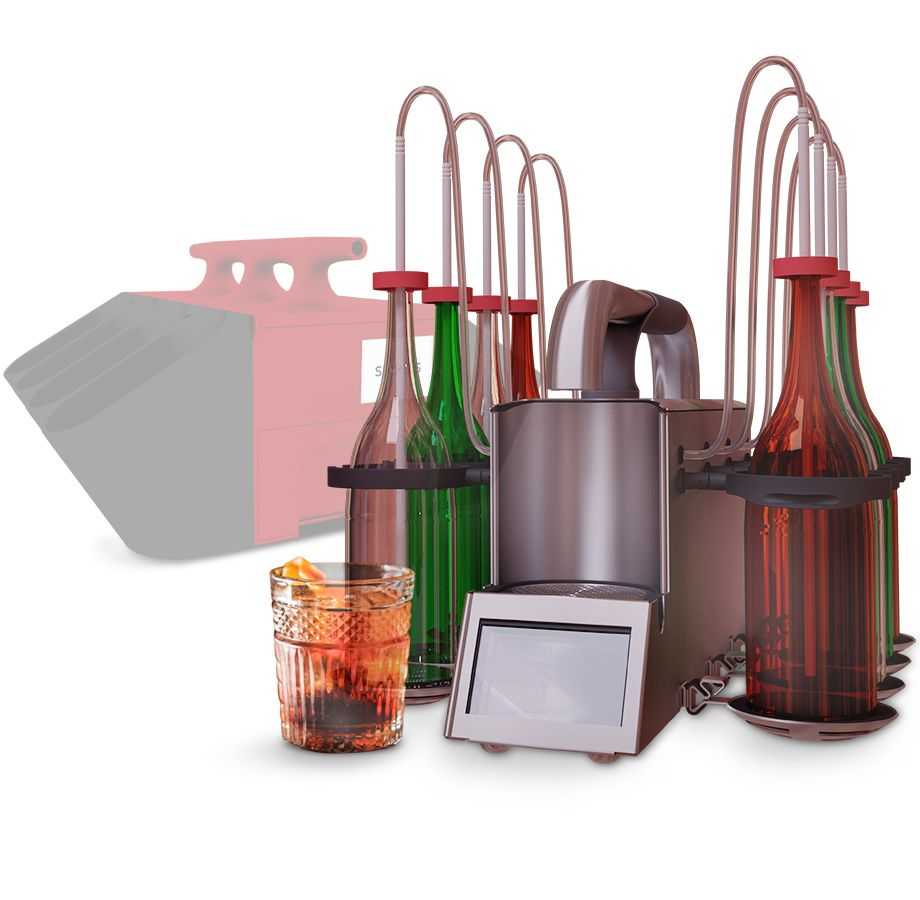
\includegraphics[width=0.35\textwidth]{graphics/Spirits.JPG}
	\caption{Spirits-Cocktailmaschine \cite{koths_spirits_nodate}}
	\label{fig:Spirits_Cocktailmaschine}
\end{figure}
		\subsubsection{Der Cocktailmixer}\label{subsubsec:Der_Cocktailmixer}
\paragraph{Aufbau}\label{subsubsec:Aufbau_Der_Cocktailmixer}\mbox{}\\

Der Cocktailmixer ist ein 1m breites und 76cm hohes Küchengerät auf Rollen. Im Unterschrank können bis zu 28 Zutaten gelagert werden. Das Gehäuse besteht aus Edelstahl und ist sehr aufwendig und professionell gestaltet, sodass es in einer Restaurantküche einen Platz finden könnte. Die Schläuche führen im Schrank zum Flüssigkeitsauslass und sind bei geschlossenen Fronttüren nicht sichtbar. Gemäss Hersteller können 14-40 Getränkeanschlüsse realisiert werden. Die Behälter haben standardmässig ein Volumen von 5 Liter und können bei Bedarf auch auf 10 und 20 Liter erweitert werden. Über der Oberfläche befindet sich ein einziger Flüssigkeitsauslass. Die Maschine kann in der bestehenden Theke eingebaut werden. Gesteuert wird die Maschine von einer SPS-Steuerung, welche eine hohe Verlässlichkeit ohne Ausfällen gewährleisten soll.\cite{bg_innovation_cocktailmaschine_nodate}

\paragraph{Bedienung}\label{subsubsec:Bedienung_Der_Cocktailmixer}\mbox{}\\

Die Bedienung geschieht mittels einem 7’’ Touch-Display, welches sich über dem Flüssigkeitsauslass befindet. Das selbe Display wird auch in der Schifffahrt gebraucht und ist deswegen besonders robust und Flüssigkeitsresistent.\cite{bg_innovation_cocktailmaschine_nodate}

\paragraph{Technische Daten}\label{subsubsec:Technische_Daten_Der_Cocktailmixer}\mbox{}\\

\begin{tabular}{@{}llp{0.6\textwidth}}
    Zeit für einen Cocktail: & : & Für die Zubereitung eines Cocktails benötigt die Maschine lediglich   3-5 Sekunden. Somit sind bis zu 300 Cocktails in der Stunde möglich. \cite{bg_innovation_cocktailmaschine_nodate}\\
    \hline
    Anzahl verschiedene Cocktails: & : & Abhängig von der Anzahl Getränkeanschlüssen können mehr oder weniger Getränke zubereitet werden. Der Speicherplatz bietet jedoch Platz für 500 gespeicherte Cocktails. Die Cocktails können frei programmiert und gespeichert werden, genauso wie die Dosierungseinstellungen. Dies kann direkt an der Maschine vorgenommen werden und benötigt keiner Software. \cite{bg_innovation_cocktailmaschine_nodate}\\ 
    \hline
    Stromversorgung: & : & Der Cocktailmixer benötigt in jedem Fall einen Festanschluss an das Stromnetz. \cite{bg_innovation_cocktailmaschine_nodate}\\
\end{tabular}

\paragraph{Reinigung}\label{subsubsec:Reinigung_Der_Cocktailmixer}\mbox{}\\

Über die Reinigung wurden keine Angaben gefunden.

\paragraph{Sonstiges}\label{subsubsec:Sonstiges_Der_Cocktailmixer}\mbox{}\\

Die Erweiterung der Flüssigkeiten und Pumpen kann jeweils in Zweierschritten geschehen. In den für die Flüssigkeiten vorgesehenen Behältern ist eine Füllstanderkennung eingebaut. Der Support ist sehr ausführlich, es gibt Schulungen in der Software der Cocktailmaschine und die Maschine wird inklusive An- und Abfahrt aufgebaut. Das verwendete Material, worin die Getränke gelagert werden, sind lebensmittelzertifiziert.\cite{bg_innovation_cocktailmaschine_nodate}

\begin{figure}[h]
	\centering
	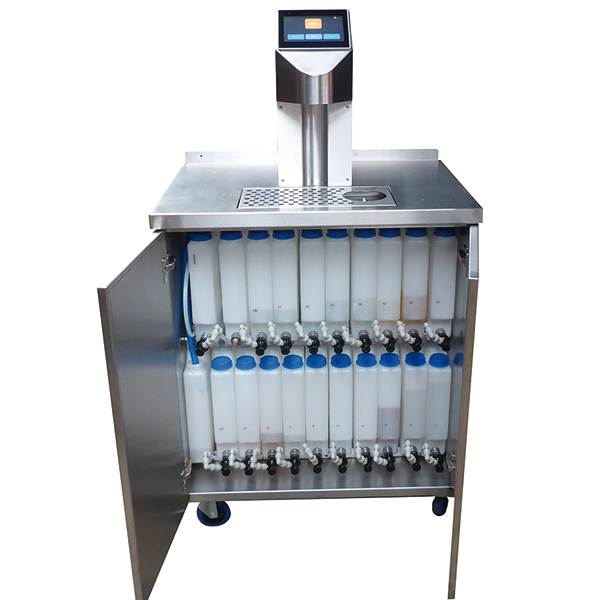
\includegraphics[width=0.4\textwidth]{graphics/DerCocktailmixer.png}
	\caption{Der Cocktailmixer \cite{bg_innovation_cocktailmaschine_nodate}}
	\label{fig:DerCocktailmixer_Cocktailmaschine}
\end{figure}
		\subsubsection{CocktailAvenue}\label{subsubsec:CocktailAvenue}
\paragraph{Aufbau}\label{subsubsec:Aufbau_CocktailAvenue}\mbox{}\\

Die Maschine CocktailAvenue besteht aus einer Rückwand, an der die Getränkeflaschen mit dem Flaschenhals nach unten montiert werden können. In der Rückwand ist ein Touchpad verbaut, über welches die Cocktails ausgewählt werden können. Das Glas wird gefüllt, indem es auf einem Schlitten unter die Flaschen fährt und dann die Getränke eingefüllt werden. Der Schlitten wird mittels einem Zahnriemen hin und her gefahren. Das Auffüllen geschieht nicht mit Pumpen, sondern mit reiner Schwerkraft. Dosiert werden die Getränke mit Dosiergeräten, wie man sie aus den Bars kennt. Dabei wird eine Fixe Dosis (meist 2cl) hinaus gelassen. Die Dosiereinheit wird geöffnet, indem ein Hubzapfen aus der Halterung des Schlittens nach oben gefahren wird. Es gibt jedoch auch zwei Hahnen, aus denen Getränke hinausgelassen werden können. Vermutlich werden dort Pumpen eingesetzt.\cite{igus_automatisiertes_nodate}

\paragraph{Bedienung}\label{subsubsec:Bedienung_CocktailAvenue}\mbox{}\\

Die Bedienung geschieht über das Touchpad, welches in der Rückwand verbaut ist.\cite{igus_automatisiertes_nodate}

\paragraph{Technische Daten}\label{subsubsec:Technische_Daten_CocktailAvenue}\mbox{}\\

\begin{tabular}{@{}llp{0.6\textwidth}}
    Zeit für einen Cocktail: & : & Für die Zubereitung eines Cocktails braucht die Maschine gemäss einem Beispiel eines Youtube-Videos 25 Sekunden. \cite{cocktail_1_2017}\\
    \hline
    Anzahl verschiedene Cocktails: & : & Es wurden keine Angaben über die Anzahl verschiedene Cocktails gefunden. \\ 
    \hline
    Stromversorgung: & : & Der Cocktailmixer benötigt in jedem Fall einen Festanschluss an das Stromnetz.\cite{igus_automatisiertes_nodate} \\
\end{tabular}

\newpage

\paragraph{Reinigung}\label{subsubsec:Reinigung_CocktailAvenue}\mbox{}\\

Die Reinigung gestaltet sich bei der CocktailAvenue ziemlich einfach. Da es keine Pumpen und Schläuche gibt, entfällt ein sehr grosser Teil. Einzig die Dosiergeräte müssen zwischendurch demontiert und sauber gemacht werden. Auch der mechanische Aufbau der Schiene unterhalb der Getränke wurde so konzipiert, dass eine Reinigung sehr einfach ist und eventuelle Verunreinigungen den Betrieb nicht beeinflussen.\cite{igus_automatisiertes_nodate}

\paragraph{Sonstiges}\label{subsubsec:Sonstiges_CocktailAvenue}\mbox{}\\

Die Antriebstechnik geschieht mit einer Zahnriemenachse. Sie besteht aus einem Aluprofil. Die Achse muss nicht geschmiert werden, was demnach bei Anwendungen mit hohen Hygieneanforderungen sehr vorteilhaft ist. Ebenso wird so ein wartungsfreier Betrieb gewährleistet. Der Antrieb wird mit einem Schrittmotor realisiert, was eine vibrationslose Bewegung garantiert. Damit die Kabel bei Bewegungen sauber geführt und nicht geknickt werden, wird eine Kabelkette verwendet. Zukünftig plant der Hersteller eine Erweiterung der modular aufgebauten Baureihe. Mittlerweile gibt es auch eine Version, bei der die Antriebsachse im Gehäuse verbaut ist. Die exakte Positionierung des Schlittens unter den Flaschen muss nicht sehr genau sein, da die Achse nach jeder Zubereitung wieder den Ausgangs- und Referenzpunkt anfährt. \cite{igus_automatisiertes_nodate}

\begin{figure}[h]
	\centering
	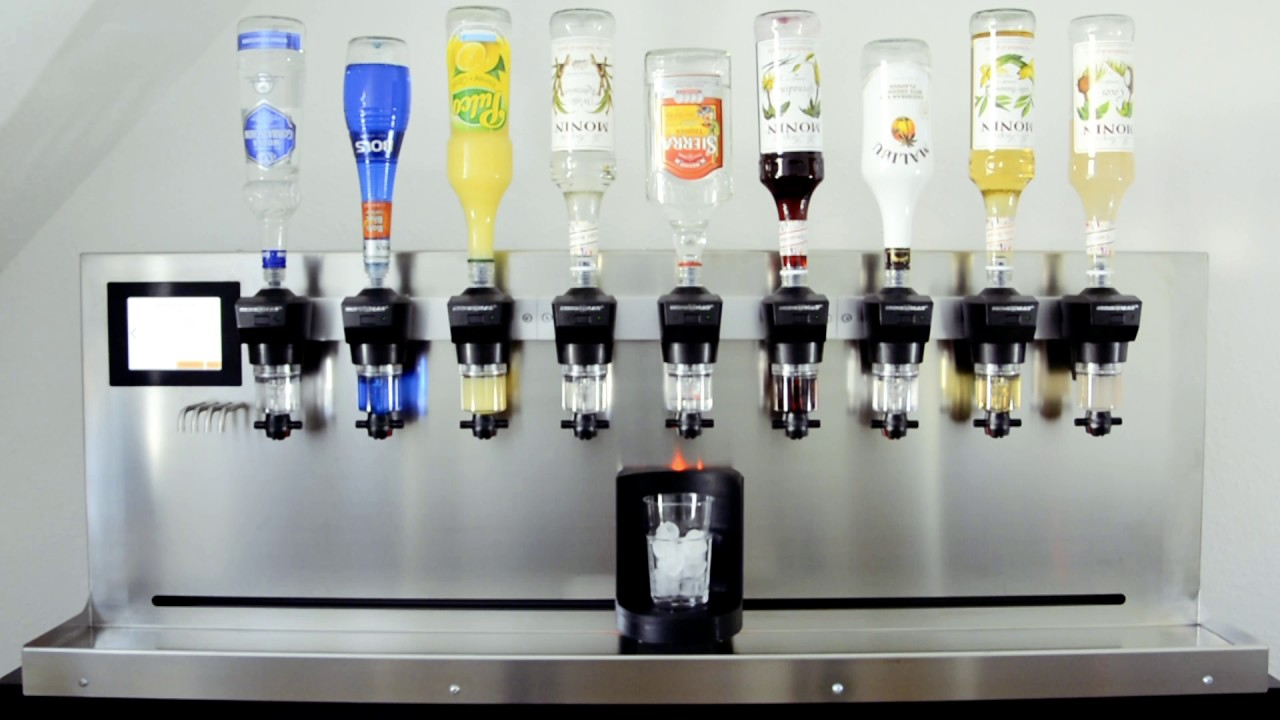
\includegraphics[width=0.5\textwidth]{graphics/CocktailAvenue.jpg}
	\caption{CocktailAvenue \cite{igus_automatisiertes_nodate}}
	\label{fig:CocktailAvenue_Cocktailmaschine}
\end{figure}
		\subsubsection{myRocktail}\label{subsubsec:myRocktail}

\paragraph{Aufbau}\label{subsubsec:Aufbau_myRocktail}\mbox{}\\

Bei my Rocktail handelt es sich um eine mietbare Cocktailmaschine, welche die Cocktails mittels eines Roboterarms zusammenmixt. Dabei kann er aus bis zu zwölf Zutaten den gewünschten Cocktail zubereiten. Die Maschine ist mobil aufgebaut und kann mittels Räder verschoben werden. Die Front der Maschine ist halbrund aufgebaut, wobei sich die Getränkeflaschen in dieser Rundung auf der Oberseite befinden. Diese sind mit dem Flaschenhals nach unten montiert, so dass das Getränk mittels automatischer Dosierkappe in das Glas abgefüllt werden kann. In der Mitte des Gerätes befindet sich zudem ein Getränkeauslass, welcher das gewünschte Süssgetränk oder Wasser hinzu mischt. \cite{myrocktail.de_home_nodate}

\newpage
\paragraph{Bedienung}\label{subsubsec:Bedienung_myRocktail}\mbox{}\\

Der Kunde kann mittels eines Touch-Displays das gewünschte Getränk auswählen und stellt dann sein Glas auf den dafür vorgesehenen Platz des Roboterarms. Danach fährt dieser die gewünschten Glaspositionen mit dem Glas an und befüllt dieses mittels den automatischen Dosierkappen mit der gewünschten Menge des Getränks. \cite{myrocktail.de_home_nodate} \cite{cnc_automation_wurfel_myrocktail_2017}


\paragraph{Technische Daten}\label{subsubsec:Technische_Daten_myRocktail}\mbox{}\\

\begin{tabular}{@{}llp{0.6\textwidth}}
    Zeit für einen Cocktail: & : & Eine Zubereitungszeit wird nicht explizit angegeben. Allerdings kann gemäss eines Videos entnommen werden, dass die Zubereitungszeit ungefähr 80 Sekunden dauert. \cite{cnc_automation_wurfel_myrocktail_2017} \\
    \hline
    Anzahl verschiedene Cocktails: & : & Es kann zwischen vier alkoholischen und vier nicht alkoholischen Getränken ausgewählt werden. Dabei besteht jedoch auf Kundenwunsch die Möglichkeit eigene Kreationen zu erschaffen. \\ 
    \hline
    Stromversorgung: & : & Es konnten keine Informationen zur Stromversorgung ausfindig gemacht werden. \\
\end{tabular}

\paragraph{Reinigung}\label{subsubsec:Reinigung_myRocktail}\mbox{}\\

Die Endreinigung wird manuell durch das Servicepersonal durchgeführt. Ob dabei ein automatischer Reinigungsmodus existiert konnte nicht ausfindig gemacht werden. Allerdings wird auf dem Prospekt mit einer einfachen Reinigung geworben. \cite{myrocktail.de_home_nodate}

\begin{figure}[h!]
	\centering
	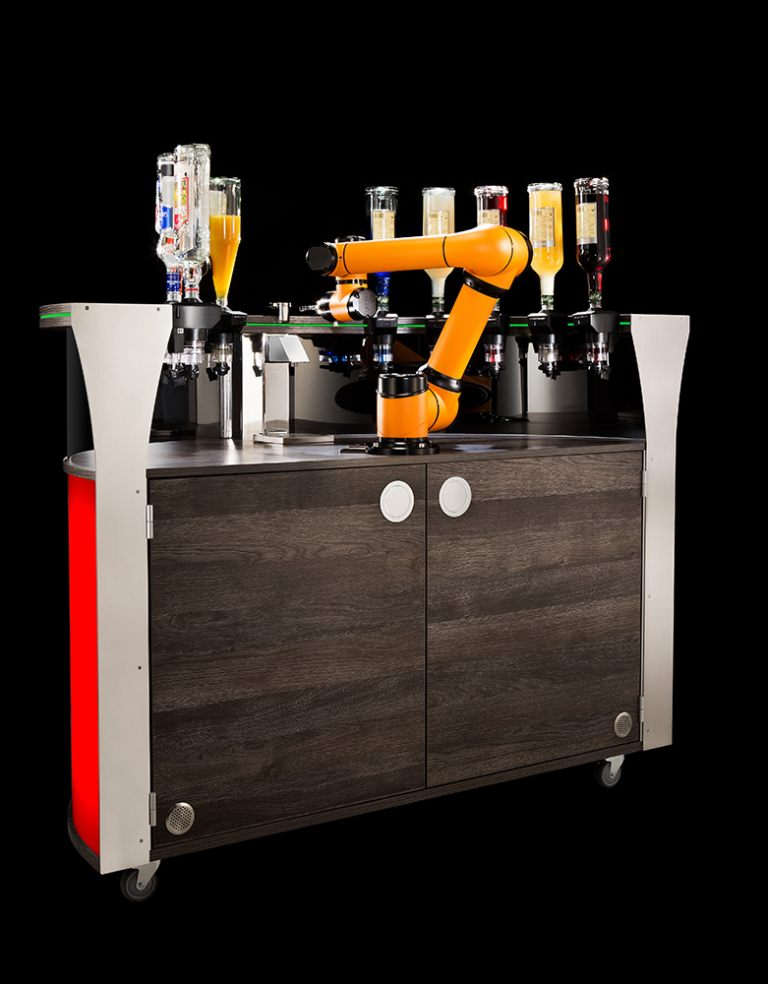
\includegraphics[width=0.3\textwidth]{graphics/myRocktail.jpg}
	\caption{myRocktail \cite{myrocktail.de_home_nodate}}
	\label{fig:myRocktail_Cocktailmaschine }
\end{figure}
		
\clearpage
\subsection{Entscheidungfindung des Aufbaus}\label{subsec:Entscheidungfindung_des_Aufbaus}

Für die Entscheidungsfindung des Aufbaus wird eine Tabelle \ref{tab:Cocktailmaschinen_Vergleich} erstellt, welche die Vor- und Nachteile der Maschinen aufzeigt.
\newline

\begin{table}[h!]
\begin{tabularx}{\textwidth}{|l|X|X|}
\hline

\textbf{Cocktailmaschine:} & \textbf{Vorteile:} & \textbf{Nachteile:} 
\\
\hline

Spirits &

\begin{itemize}[leftmargin=0.3cm,label={--}]
\item Schnelle Zubereitung (ca. 20s)
\item Mobiler Aufbau
\item Modularer Aufbau
\item Einfache Bedienung via App
\item Abspielen von Musik
\item Einfache Reinigung
\end{itemize}   &

\begin{itemize}[leftmargin=0.3cm,label={--}]
\item Kein Showeffekt für Befüllung
\end{itemize}   \\
\hline

Der Cocktailmixer & 

\begin{itemize}[leftmargin=0.3cm,label={--}]
\item Sehr schnelle Zubereitung (ca. 3-5s)
\item Mobiler Aufbau auf Rollen
\item Einfache Bedienung via Touchpad
\item Riesige Getränkeauswahl
\item Grosses Fassungsvolumen
\end{itemize}   & 

\begin{itemize}[leftmargin=0.3cm,label={--}]
\item Kein Showeffekt für Befüllung
\item Grosse, sperrige Maschine
\item Keine Appsteuerung
\item Grosser Reinigungsaufwand
\item Kein Showeffekt
\end{itemize}   \\
\hline

Cocktail Avenue   & 

\begin{itemize}[leftmargin=0.3cm,label={--}]
\item Schnelle Zubereitung (ca. 25s)
\item Einfache Bedienung via Touchpad
\item Einfacher Flaschenwechsel
\item Präzise Dosierung
\item Grosser Showeffekt durch Schlitten
\item Einfache Reinigung
\end{itemize}   &

\begin{itemize}[leftmargin=0.3cm,label={--}]
\item Längere Zubereitungszeit durch Bewegung
\item Benötigt viel Platz
\item Stark begrenzte Getränkeauswahl
\end{itemize}   \\
\hline

myRocktail &

\begin{itemize}[leftmargin=0.3cm,label={--}]
\item Grosser Showeffekt durch Roboterarm
\item Einfache Bedienung via Touchpad
\item Einfacher Flaschenwechsel
\item Präzise Dosierung
\item Mobiler Aufbau auf Rollen
\item Einfache Reinigung
\end{itemize}   &

\begin{itemize}[leftmargin=0.3cm,label={--}]
\item Längere Zubereitungszeit durch Bewegung (ca. 80s)
\item Benötigt viel Platz
\item Stark begrenzte Getränkeauswahl
\end{itemize}   \\
\hline
\end{tabularx}
\caption{Cocktailmaschinen Vergleich}
\label{tab:Cocktailmaschinen_Vergleich}
\end{table}
\newpage
Die Cocktailmaschine soll einige Anforderungen erfüllen. Aus diesen resultiert dann die komplette Entscheidungsfindung bezüglich des Aufbaus. Dies ist zum einen der Showeffekt. Die Cocktailmaschine soll ein Hingucker sein und dem Benutzer etwas für das Auge bieten. Daher soll das Glas zu den verschiedenen Befüllgetränken befördert werden, um diese zu befüllen. Ausserdem soll es weniger als eine Minute dauern, bis ein Cocktail erstellt ist. Da der Roboterarm weit mehr als eine Minute benötigt um einen Cocktailzu erstellen, führt zur Entscheidung ein Förderband einzusetzen, wie es bei der Cocktail Avenue der Fall ist. Weiter soll dem Benutzer eine möglichst Benutzerfreundliche Bedienoberfläche geboten werden. Diese soll so intuitiv wie möglich gestaltet werden. Daher wird ein Touchscreen verbaut, wie es beim Cocktailmixer und der myRocktail der Fall ist. Von der Spirits soll die Flüssigkeitsbeförderung übernommen werden. Daher werden Pumpen, sowie Durchflussmessgeräte verbaut.   

\pagebreak
\section{Grobkonzept}\label{sec:Grobkonzept}

Das Grobkonzept soll eine Übersicht über den Aufbau der Maschine bieten. Dabei wird erläutert, aus welchen Hauptkomponenten die Cocktailmaschiene besteht und weshalb diese ausgewählt wurden. Ausserdem sollen deren technischen Daten aufgezeigt werden. 



\subsection{Blockschaltbild}\label{subsec:Blockschaltbild}

Das Blockschaltbild soll die Funktionsweise der Cocktailmaschine veranschaulichen. Dabei wird unterschieden zwischen der Steuerelektronik (MCS) und den externen Komponenten wie Netzteil, Touchscreen (HMS), Beleuchtung (ML), Pumpen, Durchflussmessgeräte, Endschalter und Motor. Aufgrund dieses Blockschaltbildes werden in den folgenden Kapitel die Hauptkomponenten ausgewählt.

\begin{figure}[h!]
	\centering
	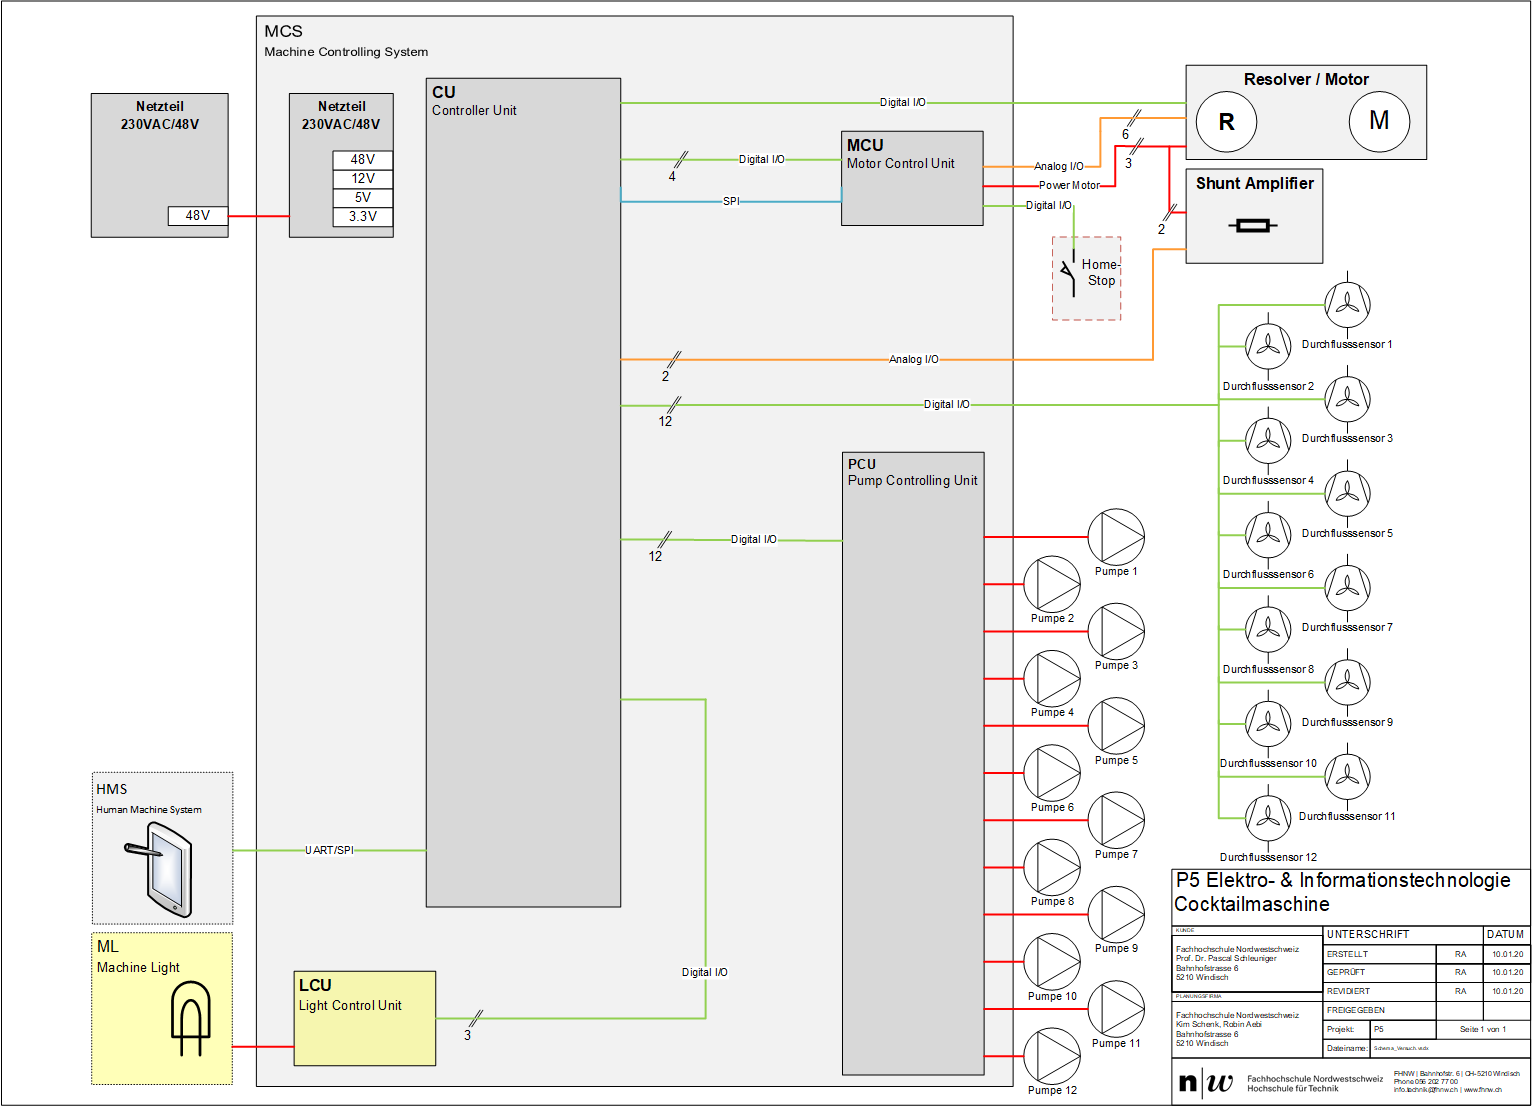
\includegraphics[angle=90, width=\textwidth]{graphics/P5-Blockschema.png}
	\caption{Blockschaltbild}
	\label{fig:Blockschaltbild}
\end{figure}  

\newpage  

%


\subsection{Motor}\label{subsubsec:Motor}

Als Motor wird ein bürstenloser Gleichstrommotor (BLDC-Motor) verwendet. Diese Bauform wurde vom betreuenden Dozent vorgegeben.
Ein BLDC-Motor zeichnet sich dadurch aus, dass er zu den Antrieben mit dem besten Verhältnis zwischen Leistung und Gewicht zählt. Ausserdem verfügt er über ein relativ hohes Drehmoment. Die Anwendung bringt bis auf die Drehlager keinen Verschleiss mit sich. Er ist zuverlässiger, effizienter und zudem noch leiser als herkömmliche Motoren \cite{imajey_consulting_engineers_pvt_ltd_brushless_nodate}. Im folgenden Kapitel soll gezeigt werden, wie solch ein Motor aufgebaut ist und nach welchem Funktionsprinzip er funktioniert.

\subsubsection{Aufbau}\mbox{}\\

Ein bürstenloser Gleichstrommotor funktioniert im Grunde nicht nach dem Prinzip eines Gleichstrommotors. Vom Aufbau her ist er gebaut wie ein Wechselstrom-Synchronmotor, wobei die Erregung mit Permanentmagneten gewährleistet wird. Beim Synchronmotor am 400V-Netz geschieht die magnetisierung der Spulen mit der sinusförmigen Netzfrequenz. Beim BLDC-Motor hingegen über die wechselnde magnetisierung mit einem Gleichstrom. Es wird folglich eine Steuerlogik benötigt, welche diesen Gleichstrom auf die Spulen schaltet. In Abbildung \ref{fig:Aufbau_Synchron_und_BLDC} wird der Aufbau beider Motoren veranschaulicht. \cite{noauthor_burstenloser_2019}

\begin{figure}[h!]
\centering
\hspace{3cm}
\subcaptionbox{3-Phasen-Synchronmotor \cite{noauthor_difference_nodate}}{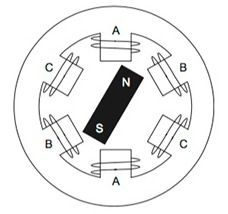
\includegraphics[height=4.5cm]{graphics/3_Phasen_Synchronmotor.jpg}}%
\hfill
\subcaptionbox{BLDC-Motor\cite{noauthor_choosing_2018}}{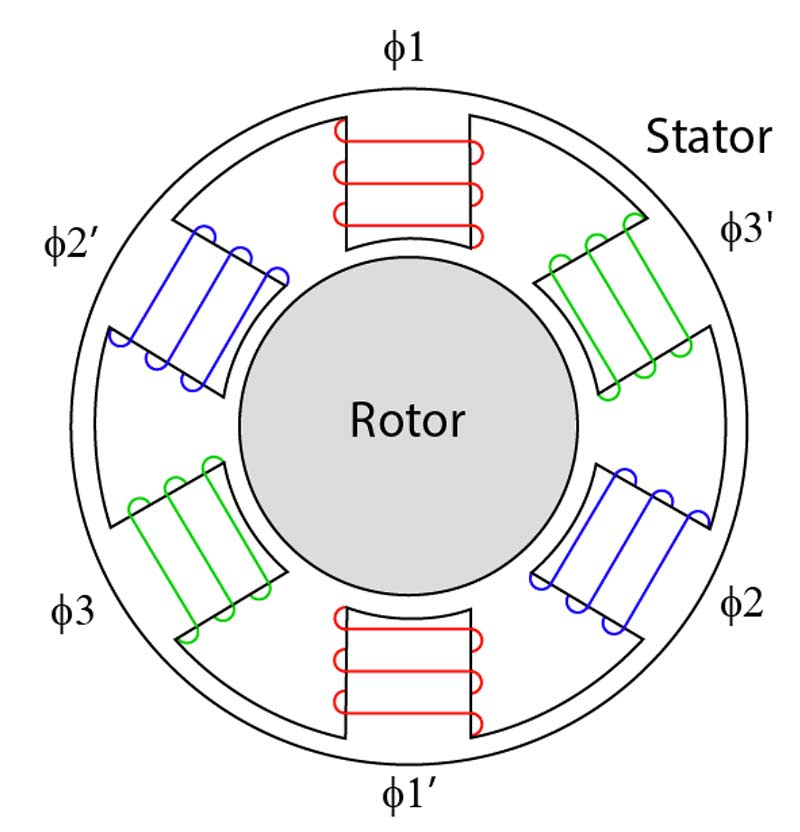
\includegraphics[height=4.5cm]{graphics/BLDC_Motor.jpg}}%
\hfill
\hspace{3cm}
\caption{Vergleich des Aufbaus zwischen Synchron- und BLCD-Motor.}
\label{fig:Aufbau_Synchron_und_BLDC}
\end{figure}

Hauptsächlich unterscheiden sich die BLDC-Motoren in Aussen- und Innenläufer.

\begin{tabbing}
\parbox[t]{.25\textwidth}{Aussenläufer} \= \parbox[t]{.75\textwidth}{Aussenläufer haben den Rotor ausserhalb des Stators (siehe Abb. \ref{fig:Kraftwirkung_BLDC_1}). Der Rotor bei Aussenläufern weist deshalb eine grössere Massenträgheit auf. Aus diesem Grund sind sie bevorzugt, wenn es darum geht zu erwartende Schwankungen in der Drehzahl oder im Drehmoment auszugleichen. \cite{bruner_burstenloser_2016} \cite{hembach_systematischer_2007}}\\
\\
\parbox[t]{.25\textwidth}{Innenläufer} \>\parbox[t]{.75\textwidth}{Innenläufer haben den Rotor auf der Innenseite des Stators (siehe Abb. \ref{fig:Aufbau_Synchron_und_BLDC}). Sie werden aufgrud der niedrigeren Trägheit für schnelle Richtugsänderungen bevorzugt.}
\end{tabbing}
\newpage
\subsubsection{Funktionsprinzip}

In Abbildung \ref{fig:Kraftwirkung_BLDC_1} sind die Spulen in der mitte statisch und bilden den Stator. Die Permanentmagnete sind am schwarzen Teil befestigt, welcher den Rotor darstellt. Durch die von einem Strom verursachte Magnetisierung der B-Spule ganz links auf der Abbildung, wird der Nord- und Südpol des Rotors im Gegenuhrzeigersinn angezogen. Die Kräftewirkung ist in der Abbildung mit einem grünen Pfeil dargestellt. Der Rotor beginnt sich zu drehen. Sobald der Rotor die Position erreicht, wie sie in der Mitte der Abbildung dargestellt wird, ändert sich die Magnetisierung von Spule B auf Spule C. Der Prozess der Anziehung und Drehung findet erneut statt und endet mit Erreichen der nächsten Position. Darauf folgt eine weitere Änderung der Magnetisierung von Spule C auf A. Wird dieser Prozess kontinuierlich wiederholt, dreht sich der Motor im Kreis.

\begin{figure}[h!]
	\centering
	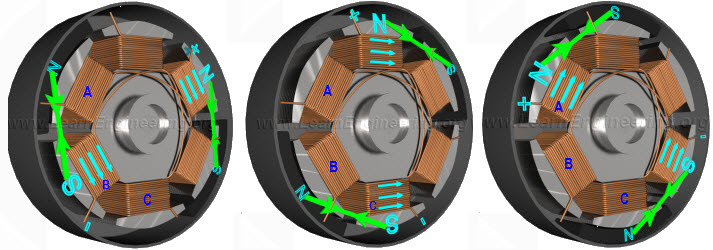
\includegraphics[height=4cm]{graphics/BLDC_Kraftwirkung_1.jpg}
	\caption{Kraftwirkung nur mit Anziehung (grün) \cite{imajey_consulting_engineers_pvt_ltd_brushless_nodate}}
	\label{fig:Kraftwirkung_BLDC_1}
\end{figure}

Würde man den Motor blockartig betreiben, hätte man nur wenige Positionen, welche angesteuert werden können. Zusätzlich können Vibrationen auftreten. Um dies zu verhindern werden die Spulen mit einem PWM-Signal gespiesen. Dies hat zur Folge, dass der Strom durch die Spulen und somit auch die Magnetisierung regulierbar ist. So kann der Motor mit feinen Positionsänderungen angesteuert werden und er verhält sich ruhiger im Betrieb. Das PWM-Signal kann beispielsweise wie in Abbildung \ref{fig:Motor_Kommuntierung_1} dargestellt generiert werden.

\begin{figure}[h!]
	\centering
	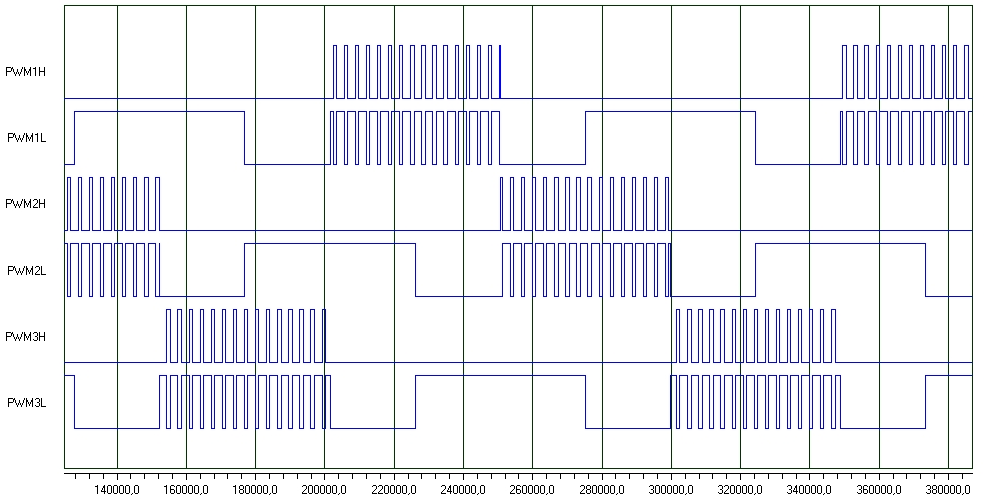
\includegraphics[width=0.8\textwidth]{graphics/Kommuntierung_BLDC_Blockkommuntierung.png}
	\caption{PWM-Signal der Kommuntierung. Das invers-PWM auf der Low-Side  wird geschaltet, um die Body-Diode zu entlasten.
	\cite{marc_bldc_2015}
	}
	\label{fig:Motor_Kommuntierung_1}
\end{figure}
\newpage
Die PWM-förmige Kommuntierungsspannung beeinflusst den Strom und somit die Magnetisierung der Spulen. Wird ein zunehmend breiteres PWM-Signal angelegt (grösserer Duty-Cycle), steigt der Strom. Wird das Signal wieder schmaler (kleinerer Duty-Cycle), sinkt der Strom. Dies ist in Abbildung \ref{fig:Motor_Kommuntierung_2} ersichtlich.

\begin{figure}[h!]
	\centering
	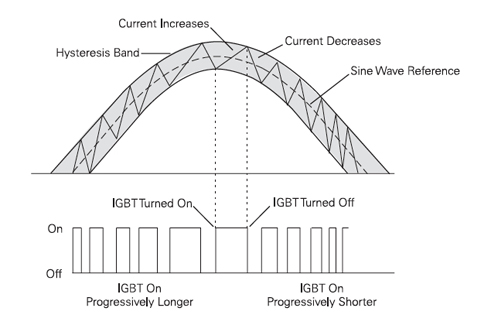
\includegraphics[width=0.8\textwidth]{graphics/Kommuntierung_BLDC_Sinus_Strom.png}
	\caption{Kraftwirkung nur mit Anziehung (grün) 
	\cite{lehane_wie_2012}
	}
	\label{fig:Motor_Kommuntierung_2}
\end{figure}
%\begin{figure}[h!]
%\centering
%\subcaptionbox{Ausgangssignal des PWM-Pins beim Einschaltvorgang.}{	\includegraphics[width=0.45\textwidth]{graphics/}}
%\hfill
%\subcaptionbox{Ausgangssignal des PWM-Pins beim Ausschaltvorgang.\label{fig:Motor_Kommuntierung_1}}{	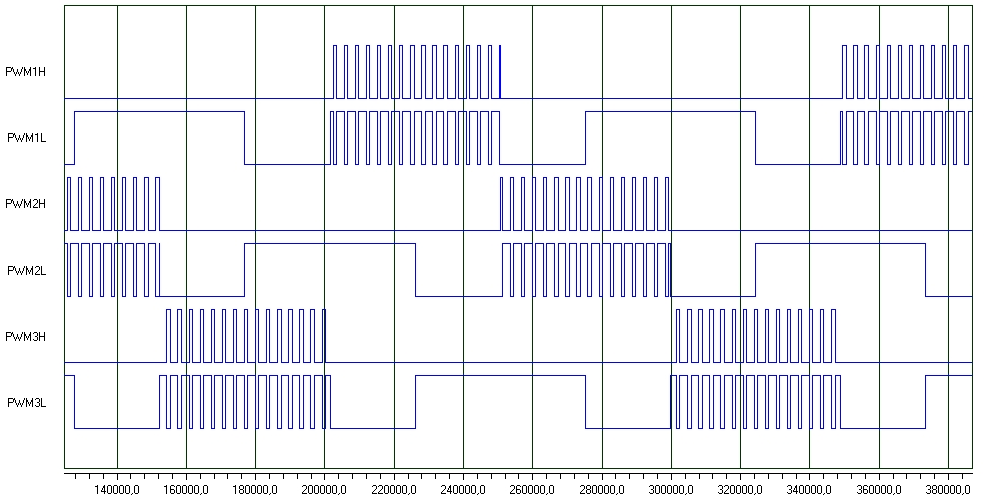
\includegraphics[width=0.45\textwidth]{graphics/Kommuntierung_BLDC_Blockkommuntierung.png}}
%\hfill
%\caption{Schematische und grafische Darstellung eines Resolvers.}
%\label{fig:Motor_Kommuntierung}
%\end{figure}

Dieser Prozess kann verstärkt werden, indem das Prinzip der Abstossung genutzt wird. Dazu werden zusätzlich die Spulen gemäss Abbildung \ref{fig:Kraftwirkung_BLDC_2} magnetisiert. Je nach Anwendung kann es aber auch möglich sein, dass man einen Rotor still halten möchte. Dazu lässt man die Spulen permanent magnetisiert, ohne das Feld zu ändern. Die Aufgabe, dies zu steuern, übernimmt der von Trinamic entwickelte TMC4672. Dessen Funktion wird in Kapitel \ref{subsec:TMC4671_EVAL_Boad} erläutert. 

\begin{figure}[h!]
	\centering
	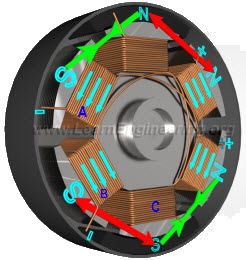
\includegraphics[height=4cm]{graphics/BLDC_Kraftwirkung_2.jpg}
	\caption{Kraftwirkung mit Anziehung (grün) und Abstossung (rot) \cite{imajey_consulting_engineers_pvt_ltd_brushless_nodate}}
	\label{fig:Kraftwirkung_BLDC_2}
\end{figure}

%Der Rotor wird foglich vom Stator ständig hinterhergezogen bzw. vorangetrieben. Mit der richtigen Ansteuerung wollen wir deshalb erreichen, dass wie in Abbildung \ref{fig:Kraftwirkung_BLDC_3} dargestellt, der Rotor wie ein Esel dem magnetischen Fluss (magnetic flux) hinterher rennt.
%
%\begin{figure}[h!]
%	\centering
%	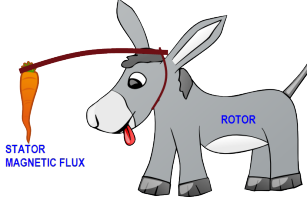
\includegraphics[height=3.5cm]{graphics/BLDC_Kraftwirkung_Esel.png}
%	\caption{Veranschaulichung Kraftwirkung \cite{imajey_consulting_engineers_pvt_ltd_brushless_nodate}}
%	\label{fig:Kraftwirkung_BLDC_3}
%\end{figure}

%\paragraph{Kommuntierung}\mbox{}\\

%Damit der Rotor der Magnetisierung nachrennen kann, braucht es ein sich änderndes Magnetfeld. In Abbildung \ref{fig:Kommuntierung_BLDC_1} wird dargestellt, wie die magnetisierung des Synchronmotors (links) und des BLDC-Motors (rechts) aussieht. Diese Aufgabe übernimmt der von Trinamic entwickelte TMC4672. Dessen Funktion wird in Kapitel \ref{subsubsec:TMC4671_EVAL_Boad} beschrieben.

%\begin{figure}[h!]
%	\centering
%	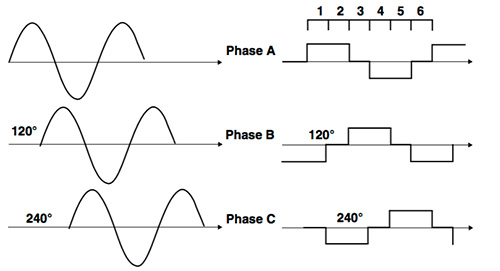
\includegraphics[height=4cm]{graphics/Sinus_und_Viereck_Signal.jpg}
%	\caption{Vergleich magnetisierung Synchronmotor und BLDC-Motor. \cite{noauthor_difference_nodate}}
%	\label{fig:Kommuntierung_BLDC_1}
%\end{figure}

%Abbildung \ref{fig:Aufbau_Synchron_und_BLDC} zeigt nochmals, dass der Synchronmotor direkt ans AC-Netz angeschlossen werden kann, während der theoretischen Aufbau für den DC-Motor noch einige komponenten benötigt.
%
%\begin{figure}[h!]
%\centering
%\subcaptionbox{3-Phasen-Synchronmotor am AC-Netz \cite{noauthor_synchronmotor_nodate}.}{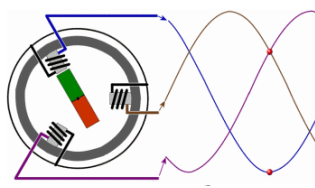
\includegraphics[height=4cm]{graphics/Synchronmotor.png}}%
%\hfill
%\subcaptionbox{BLDC-Motor am DC-Netz\cite{noauthor_choosing_2018}}{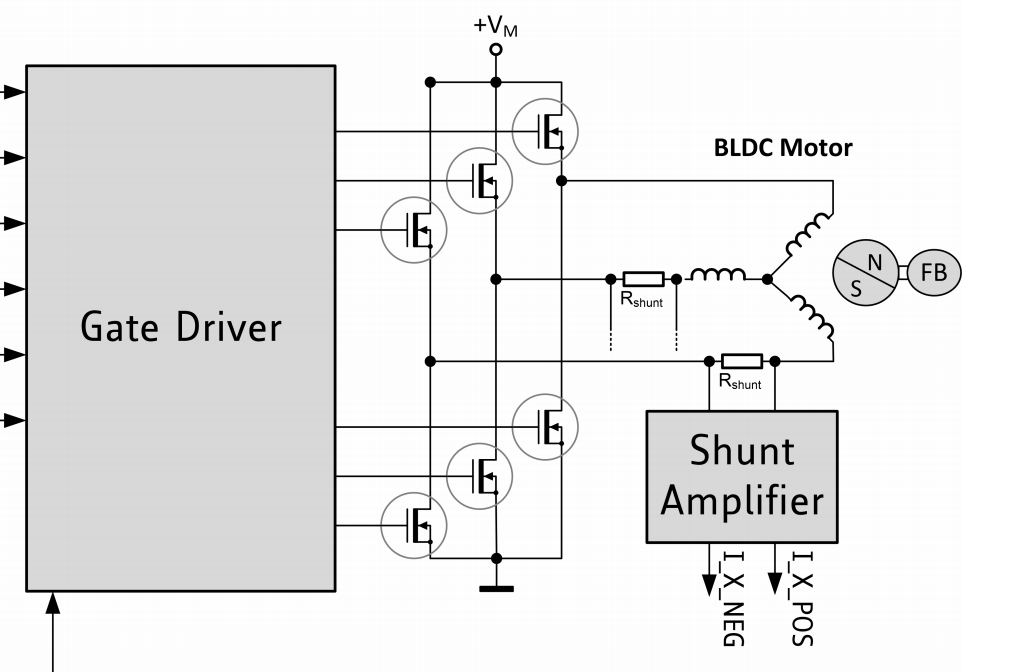
\includegraphics[height=4cm]{graphics/H_Bruecke_BLDC.png}}%
%\hfill
%\caption{Vergleich des Aufbaus zwischen Synchron- und BLCD-Motor\cite{trinamic_datasheet_2018}.}
%\label{fig:Aufbau_Synchron_und_BLDC}
%\end{figure}

%\paragraph{Motor}\label{par:Anforderungen_Motor}\mbox{}\\
%Der Motor ist folglich mit dem angegebenen Treiber für das Projekt verwendbar. Der Motor an sich hat folgende Eigenschaften:
%\begin{tabbing}
%\parbox[t]{.25\textwidth}{Anschlussspannung} \= \parbox[t]{.75\textwidth}{48 V}\\
%\parbox[t]{.25\textwidth}{Nenndrehzahl} \= \parbox[t]{.75\textwidth}{1500 rpm}\\
%\parbox[t]{.25\textwidth}{Nennmoment} \= \parbox[t]{.75\textwidth}{0.85 Nm}\\
%\parbox[t]{.25\textwidth}{Nennleistung} \= \parbox[t]{.75\textwidth}{0.13 kW}\\
%\parbox[t]{.25\textwidth}{Stillstandstrom} \= \parbox[t]{.75\textwidth}{5.41 A}\\
%\parbox[t]{.25\textwidth}{Gebersystem} \= \parbox[t]{.75\textwidth}{Resolver}\\
%\parbox[t]{.25\textwidth}{Bremse} \= \parbox[t]{.75\textwidth}{Nein}\\
%\parbox[t]{.25\textwidth}{Wellentyp} \= \parbox[t]{.75\textwidth}{Glatte Welle}\\
%\parbox[t]{.25\textwidth}{Anschluss} \= \parbox[t]{.75\textwidth}{2 SpeedTec Ready M23 Stecker, auf Motor montiert}\\
%\end{tabbing}

\subsection{Resolver}\label{subsubsec:Resolver}

Damit die genaue Lage des Rotors festgestellt werden kann, benötigt es eine Drehpositionserfassung. Im Falle des verwendeten Motors wird ein Koordinatenwandler, auf Englisch auch Resolver genannt, verwendet.
Dieser hat die Eigenschaft, eine kontinuierliche Winkellage des Rotors zu liefern und ist fest im AKM22h verbaut. Aus diesem Grund wird in diesem Kapitel die Funktion des Resolvers vertieft betrachtet.

\subsubsection{Aufbau}\label{par:Aufbau_Resolver}

Damit ein Resolver funtionieren kann, sind eine Erregerspule und zwei Sensorspulen nötig.
Weiter muss mittels Induktion die Erregungsfrequenz auf die Erregerspule übertragen werden.
Der schematische Aufbau ist in Abbildung  \ref{fig:Schematisch_Grafisch_Resolver_1} ersichtlich. Abbildung \ref{fig:Schematisch_Grafisch_Resolver_2} zeigt, wie die Komponenten zu einander stehen und wie sie (bis auf die blaue Leiterschleife) im Resolver angeordnet sind.

Das Prinzip funktioniert folgendermassen. Es wird ein periodisches Signal, vorzugsweise Sinus, auf die statische gelbe Spule gegeben. Dieses wird mittels Induktion des drehbaren Transformators an die drehbare blaue Spule übertragen. Die blaue Spule erzeugt unabhängig ihrer Lage ein magnetisches Feld anhand des Erzeugersignals und bildet so die Erregerspule. Die grüne und pinke Sensorspulen werden je nach Lage der blauen Spule unterschiedlich stark erregt und erzeugen das benötigte Signal, welches dann von der Auswertelektronik verarbeitet wird. 

\begin{figure}[h!]
\centering
\subcaptionbox{Schematische Darstellung Resolver\cite{noauthor_wie_nodate}\label{fig:Schematisch_Grafisch_Resolver_1}}{	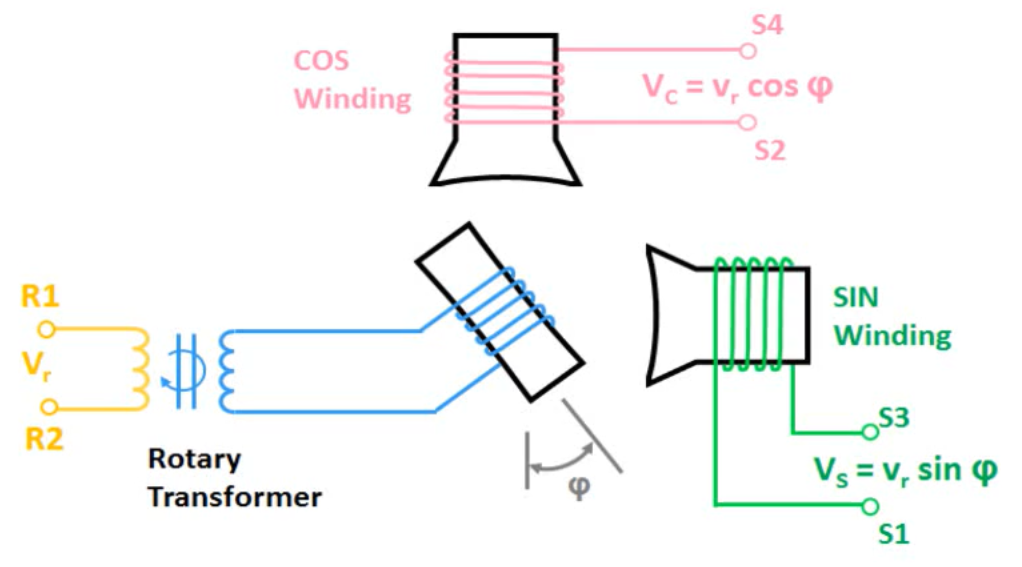
\includegraphics[width=0.45\textwidth]{graphics/Resolver_1.png}}
\hfill
\subcaptionbox{Grafische Darstellung Resolver\cite{noauthor_wie_nodate}\label{fig:Schematisch_Grafisch_Resolver_2}}{	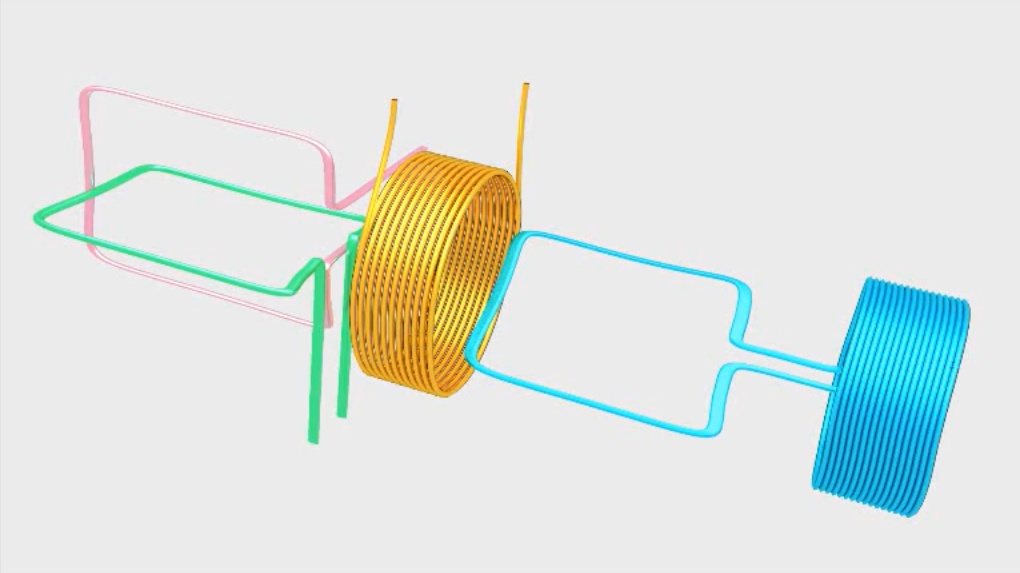
\includegraphics[width=0.45\textwidth]{graphics/Resolver_2.png}}
\hfill
\caption{Schematische und grafische Darstellung eines Resolvers.}
\label{fig:Schematisch_Grafisch_Resolver}
\end{figure}

\subsubsection{Funktionsweise}\label{par:Funktionsweise_Resolver}

Steht der Rotor wie in Abbildung \ref{fig:Position_Grafisch_0} bei 0$^\circ$, so liegt die drehbare blaue Leiterschleife so, dass der von ihr ausgehende magnetische Fluss nur eine Wirkung auf die pinke Leiterschleife hat (siehe Abbildung \ref{fig:Darstellung_Grafisch_0}). Das Erregersignal wird folglich praktisch nur von der cos-Windung wahrgenommen, wie in Abbildung \ref{fig:Signal_Grafisch_0} ersichtlich ist.

\begin{figure}[h!]
\centering
\subcaptionbox{Grafische Lage der Spulen\cite{noauthor_wie_nodate}\label{fig:Darstellung_Grafisch_0}}{	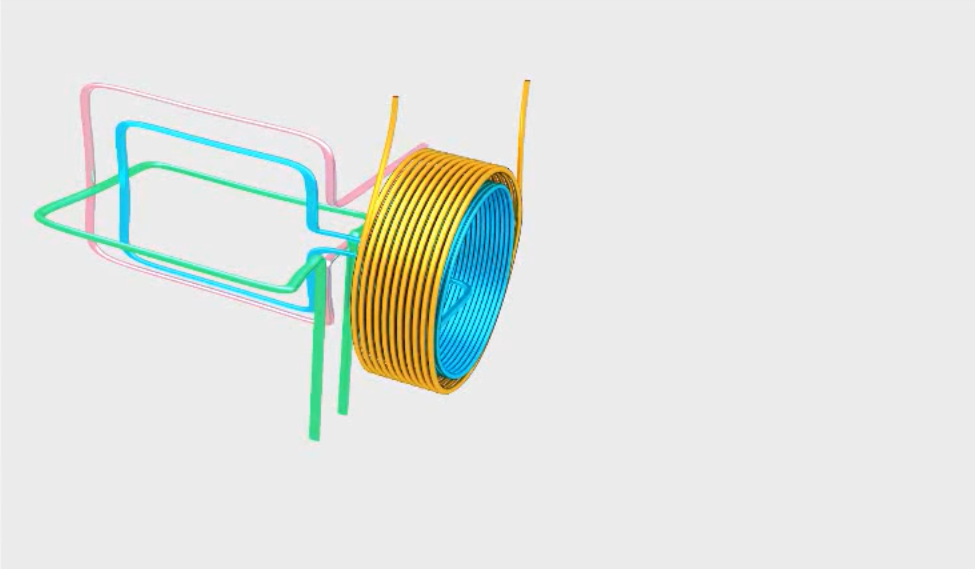
\includegraphics[width=0.3\textwidth]{graphics/Resolver_3.png}}
\hfill
\subcaptionbox{Signalverläufe der Spulen\cite{noauthor_wie_nodate}\label{fig:Signal_Grafisch_0}}{	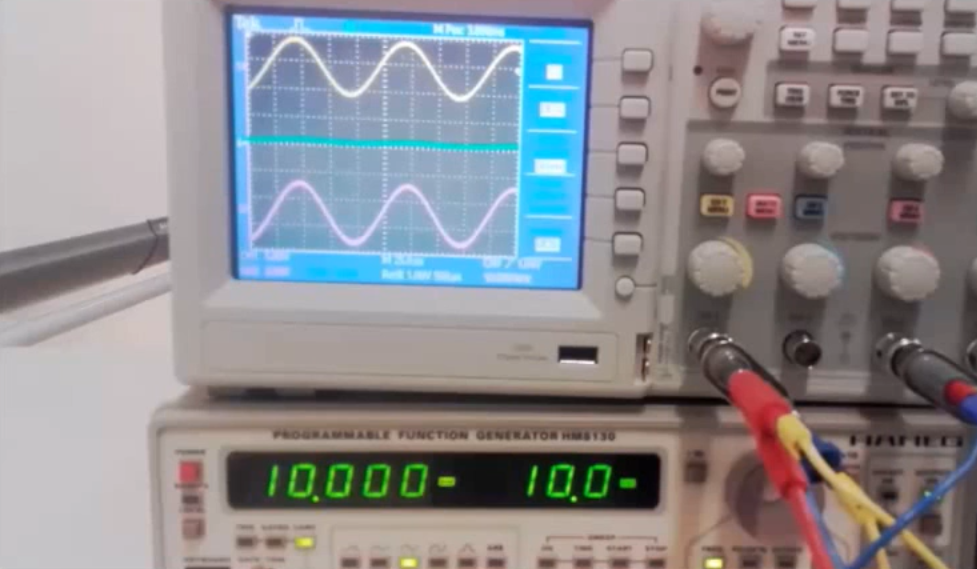
\includegraphics[width=0.3\textwidth]{graphics/Resolver_5.png}}
\hfill
\subcaptionbox{Position des Resolvers\cite{noauthor_wie_nodate}\label{fig:Position_Grafisch_0}}{	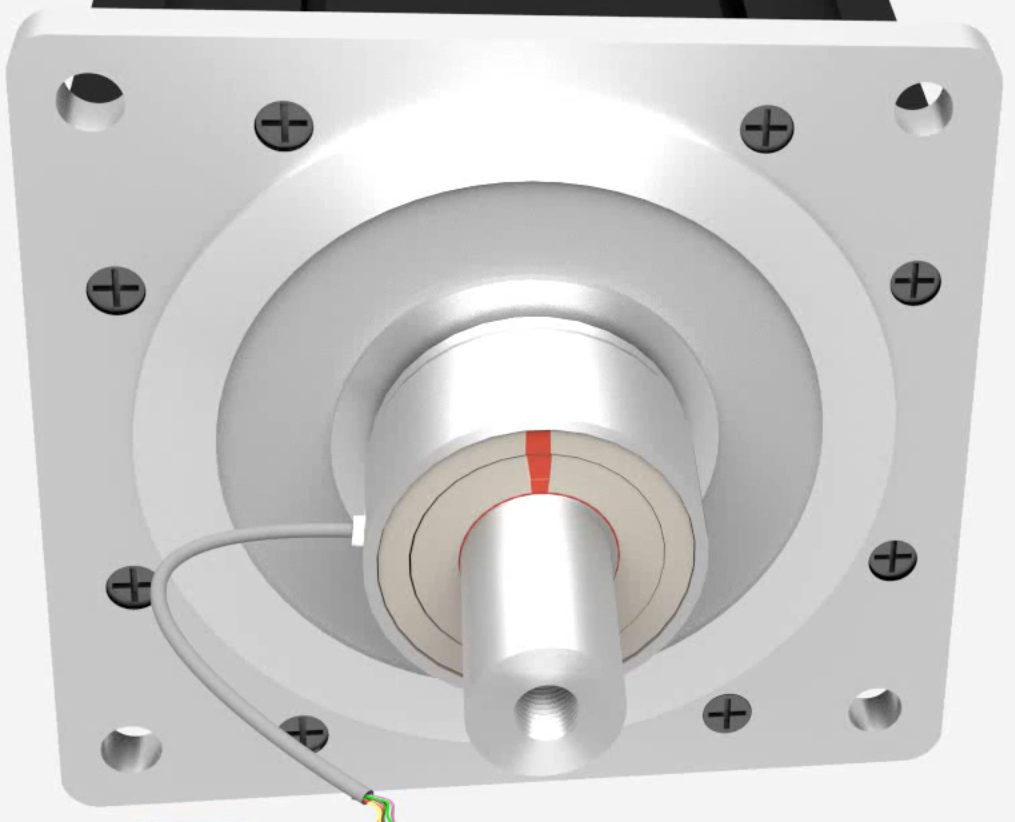
\includegraphics[width=0.3\textwidth]{graphics/Resolver_7.png}}
\hfill
\caption{Gegebenheiten bei Achsenstellung 0$^\circ$.}
\label{fig:Darstellungen_0_Grad}
\end{figure}

Steht der Rotor wie in Abbildung \ref{fig:Position_Grafisch_90} bei 90$^\circ$, so liegt die drehbarebare blaue Leiterschleife so, dass der von ihr ausgehende magnetische Fluss nur eine Wirkung auf die grüne Leiterschleife hat (siehe Abbildung \ref{fig:Darstellung_Grafisch_90}). Das Erregersignal wird folglich praktisch nur von der sin-Windung wahrgenommen, wie in Abbildung \ref{fig:Signal_Grafisch_90} ersichtlich.

\begin{figure}[h!]
\centering
\subcaptionbox{Grafische Lage der Spulen\cite{noauthor_wie_nodate}\label{fig:Darstellung_Grafisch_90}}{	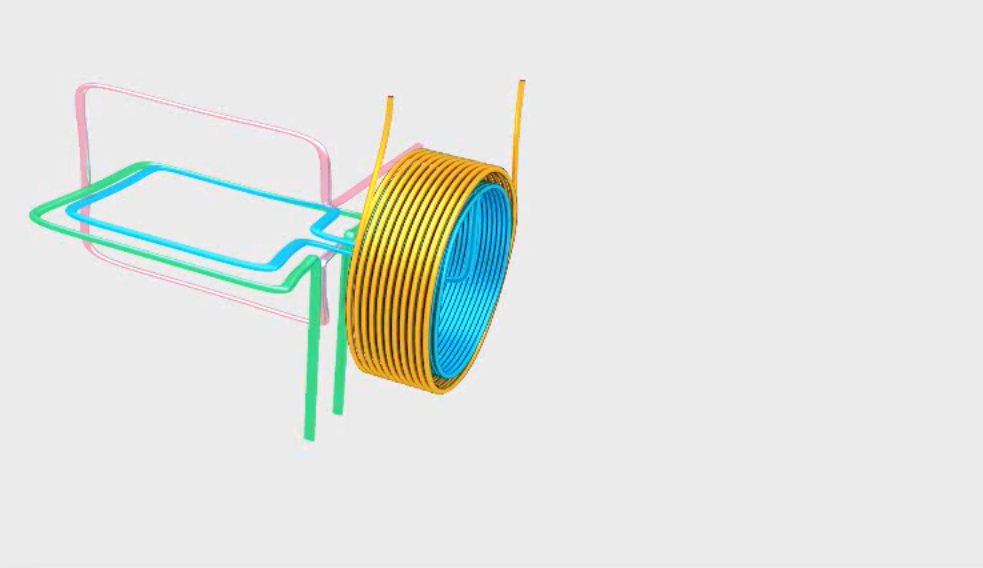
\includegraphics[width=0.3\textwidth]{graphics/Resolver_4.png}}
\hfill
\subcaptionbox{Signalverläufe der Spulen\cite{noauthor_wie_nodate}\label{fig:Signal_Grafisch_90}}{	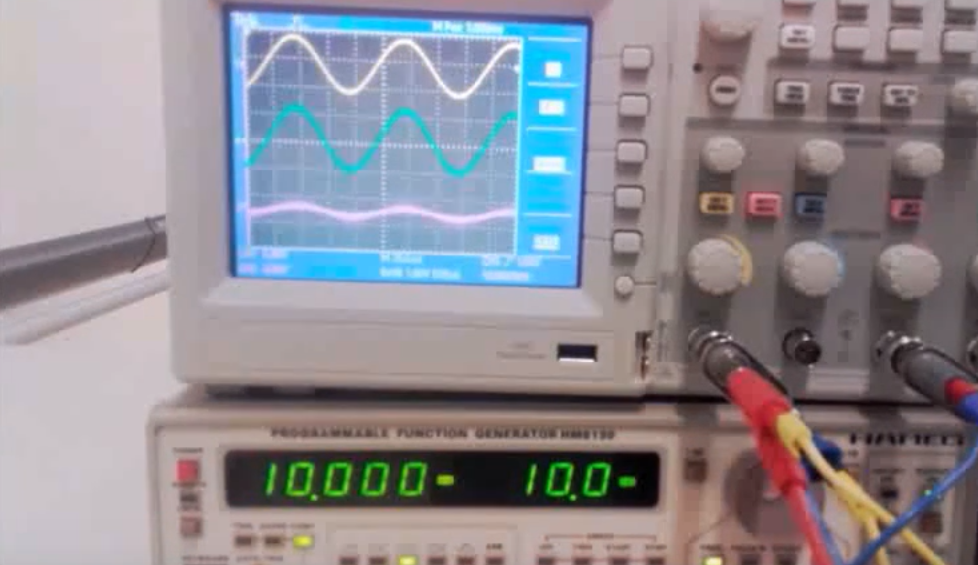
\includegraphics[width=0.3\textwidth]{graphics/Resolver_6.png}}
\hfill
\subcaptionbox{Position des Resolvers\cite{noauthor_wie_nodate}\label{fig:Position_Grafisch_90}}{	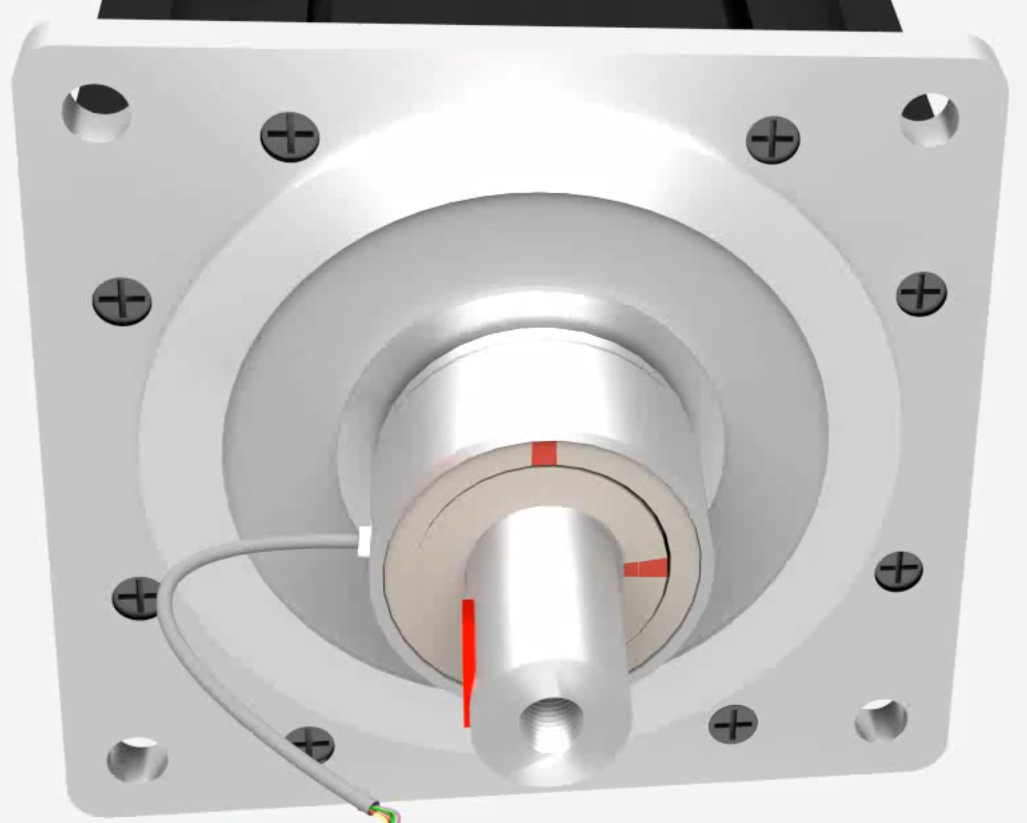
\includegraphics[width=0.3\textwidth]{graphics/Resolver_8.png}}
\hfill
\caption{Gegebenheiten bei Achsenstellung 90$^\circ$.}
\label{fig:Darstellungen_90_Grad}
\end{figure}

\subsection{TMC4671-EVAL Board}\label{subsec:TMC4671_EVAL_Boad}

Wie bereits angesprochen steuert der TMC4671 die Kommuntierungsvorgänge für den BLDC. Doch er ist noch zu viel mehr in der Lage. Der TMC4671 ist ein voll integrierter Servo-Controller, der eine feldorientierte Steuerung für BLDC/PMSM, 2-Phasen-Schrittmotoren und DC-Motoren unterstützt. Ob integrierte ADCs, Lagesensor-Schnittstellen oder Positionsinterpolatoren, alle diese in der Hardware implementierten Steuerungsfunktionen bieten einen voll funktionsfähigen Servoregler für ein breites Spektrum an Servoanwendungen. \cite{trinamic_datasheet_2018}

\subsubsection{Aufbau}\label{subsubsec:TMC4671_Aufbau}

Das komplette EVAL-Board, wie es in Abbildung \ref{fig:TMC4671_EVAL_Board} gezeigt wird, besteht aus einer Landungsbrücke (links), einem TMC4671 (mitte) und einer H-Brücke (rechts). Verbunden werden die drei Teile mittels zwei Eselsbrücken.

\begin{figure}[h!]
	\centering
	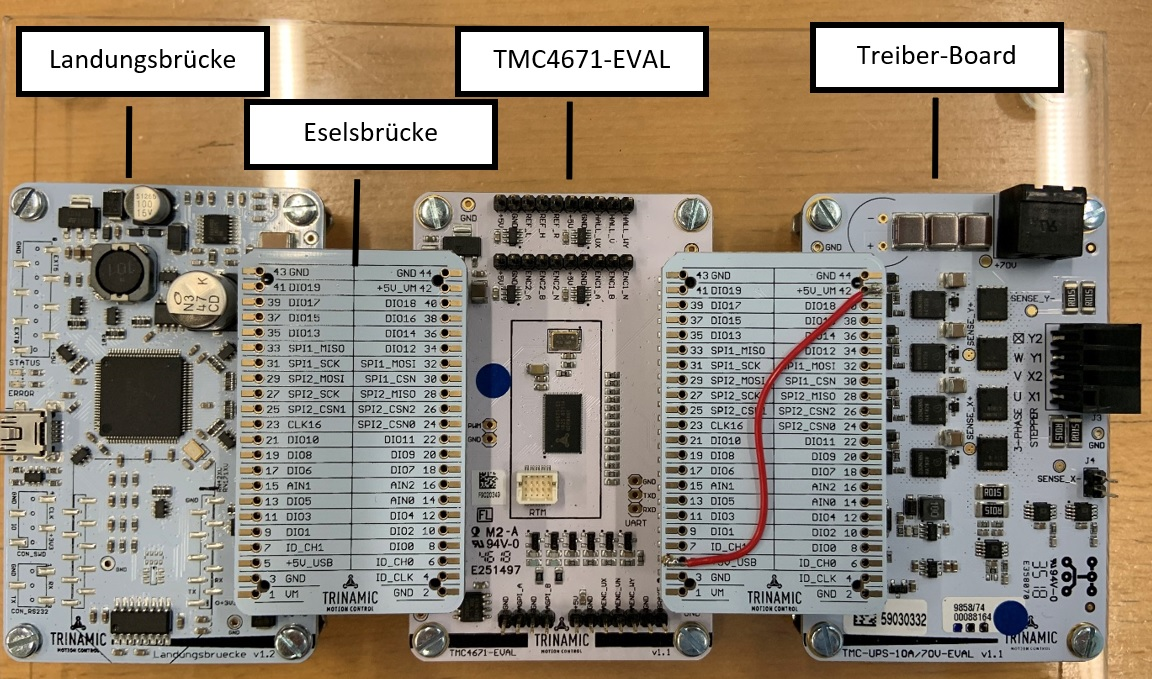
\includegraphics[width=0.6\textwidth]{graphics/TMC4671_EVAL.jpg}
	\caption{TMC4671-EVAL Board. 
	\cite{unbekannt_foc-motorenansteuerung_2019}
	}
	\label{fig:TMC4671_EVAL_Board}
\end{figure}

Die Landungsbrücke verfügt über einen USB-Anschluss, um vom Computer aus auf die Landungsbrücke zugreifen zu können. Sie bildet somit die Schnittstelle zwischen der TMCL-IDE und dem Motorentreiber, worüber die Konfiguration des Treibers stattfindet.
Der Motorentreiber stellt anhand der Konfigurationen und des Feedbacks (Spulenströme und Encodersignale) die Steuersignale für den Gate-Treiber bereit.
Der Gate-Treiber steuert die Spulenströme und magnetisiert so die Spulen des BLDC-Motors anhand der Steuersignale des Treibers. Dies wiederum verursacht eine Bewegung des Rotors.

\subsubsection{FOC}

FOC\footnote{FOC = \textbf{F}ield \textbf{O}riented \textbf{C}ontrol} ist ein Stromregelverfahren für Elektromotoren. Es reguliert die Kraft und Lage des magnetischen Feldes unter Berücksichtigung der Rotorposition, sodass der Motor das geforderte Drehmoment als Soll-Drehmoment abgibt.
FOC maximiert die Wirkleistung und minimiert die Leerlaufleistung. Dies wiederum ergibt eine Verminderung der Verlustleistung durch
intelligente Regelung. \cite{trinamic_datasheet_2018}

Auf den Rotor eines BLDC-Motors wirken zwei Kraftkomponenten. Gemäss Abbildung \ref{fig:TMC4671_EVAL_Board_FOC1} zieht eine Komponente radial in eine Richtung $I_D$ und eine andere Komponente tangential in eine Richtung $I_Q$. Die zweite Komponente $I_Q$ ist diejenige, welche ein Drehmoment auf den Rotor bringt. Der ideale Controller führt eine Regelung durch, welche einen rein drehmomenterzeugenden Strom $I_Q$ erzeugt. \cite{trinamic_datasheet_2018}

\begin{figure}[h!]
	\centering
	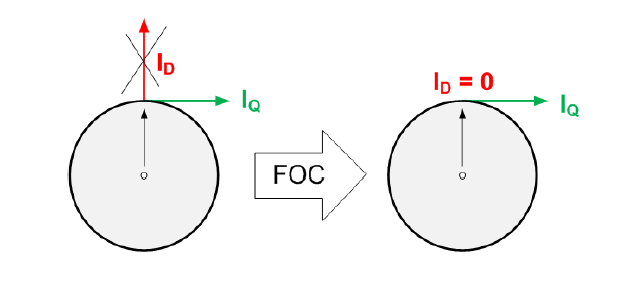
\includegraphics[width=0.6\textwidth]{graphics/FOC1.png}
	\caption{TMC4671-EVAL Board. \cite{trinamic_datasheet_2018}}
	\label{fig:TMC4671_EVAL_Board_FOC1}
\end{figure}

Der Controller verwendet für das Stromregelverfahren die drei Phasenströme des Stators, welche zusammen als Vektor betrachtet werden ($I_{U}$,$I_{V}$,$I_{W}$).
Unter Berücksichtigung der momentanen Ausrichtung des Rotors wird ein Spannungsvektor ($U_{U}$,$U_{V}$,$U_{W}$)  berechnet, sodass nur ein drehmomentbildender Strom $I_Q$ erzeugt wird (Transformation). \cite{trinamic_datasheet_2018}

Dazu sind einige statische Parameter nötig, wie z.B die Polpaarzahl des Motors, Anzahl der Impulse pro Umdrehung des verwendeten Drehgebers. Aber auch einige dynamische Parameter wie z.B die Phasenströme oder die Orientierung des Rotors. \cite{trinamic_datasheet_2018}

Von Bedeutung sind die Einstellungen der P und I Parameter zur Regelung der Phasenströme. Diese sind abhängig von den elektrischen Parametern des Motors wie z.B der Widerstand, die Induktivität, die Gegen-EMF-Konstante oder die Versorgungsspannung. \cite{trinamic_datasheet_2018}

Abbildung \ref{fig:Blockdiagramm_TMC4671} zeigt, an welcher Stelle im TMC4671 FOC (FOC23) aktiv ist. Wie zu erkennen ist, steht es mit fast allen Teilsystemen in Kontakt.
\\

\begin{figure}[h!]
	\centering
	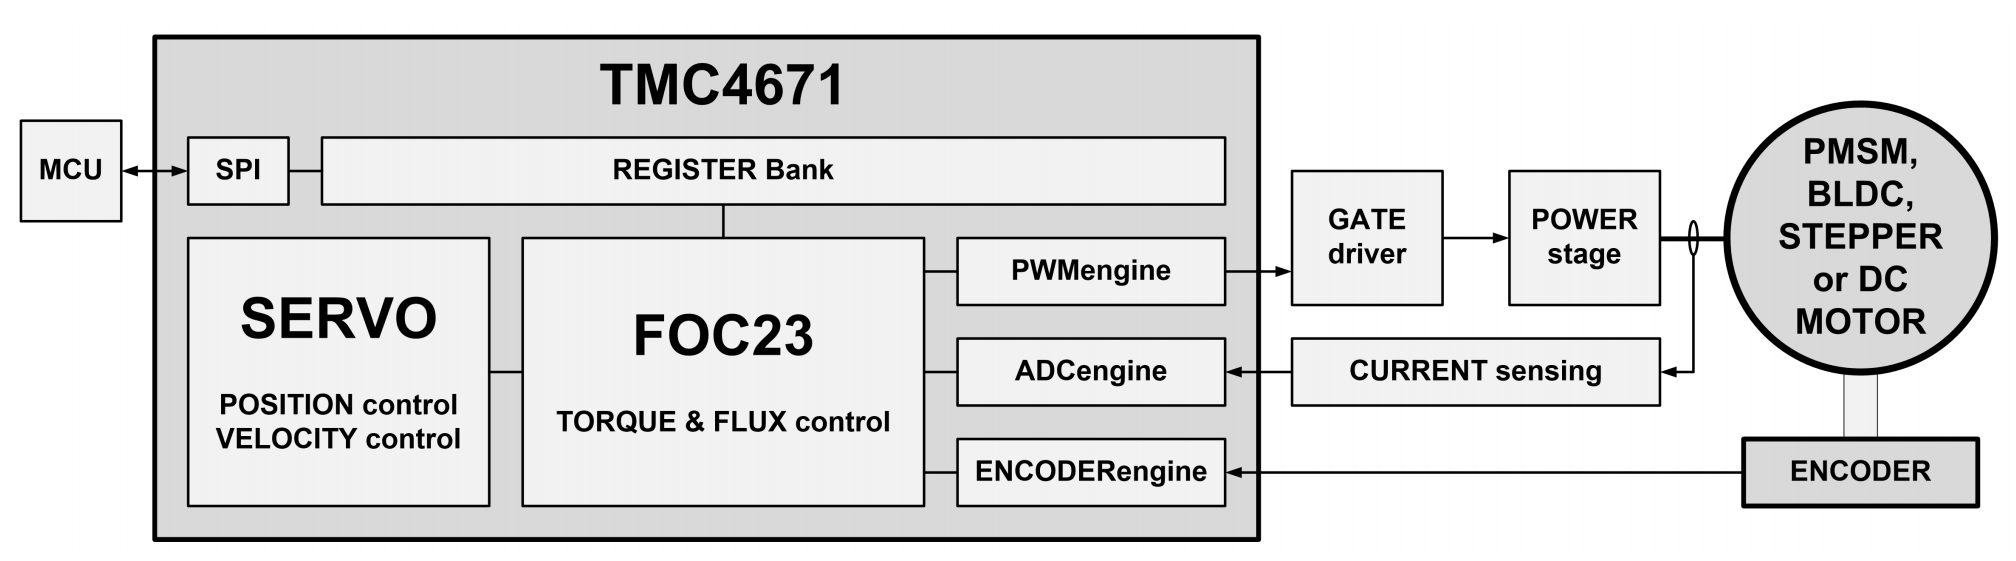
\includegraphics[width=0.7\textwidth]{graphics/Blockdiagramm_TMC4671.png}
	\caption{Standard-Anwendungs-Schaltung. \cite{trinamic_datasheet_2018}}
	\label{fig:Blockdiagramm_TMC4671}
\end{figure}
\newpage

\subsubsection{Park \& Clarke}

Für das Stromregelverfahren werden die Funktionen Clarke, Park, iClarke und iPark verwendet. Im Folgenden wird gezeigt, wie sie im Zusammenhang mit dem drehmomentgebenden Strom, den Phasenströmen, den Phasenspannungen und den PI-Parameter stehen. In Abbildung \ref{fig:TMC4671_EVAL_Board_Park_and_Clarke} sind die Zusammenhänge grafisch dargestellt.

%\begin{tabular}{lll}
%Statorströme \textbf{($I_{U}$,$I_{V}$,$I_{W}$)}& Clarke &  Stromvektor der drei Statorströme ($I_\alpha$,$I_\beta$)\\
%Stromvektor Stator ($I_\alpha$,$I_\beta$) & Park & Momentaner Stromvektor auf Rotor ($I_Q$,$I_D$)  \\
%Stromvektor Rotor ($I_Q$,$I_D$) & PID &  Berechnete Spannungen für Rotor ($U_Q$,$U_D$)\\
%Rotorspannungen ($U_Q$,$U_D$) & iPark &  Spannungsvektor der drei Statorspannungen ($U_\alpha$,$U_\beta$)\\
%Spannungsvektor ($U_\alpha$,$U_\beta$) & iClarke &  Statorspannungen \textbf{($U_{U}$,$U_{V}$,$U_{W}$)} \\
%\end{tabular}

\begin{figure}[h!]
	\centering
	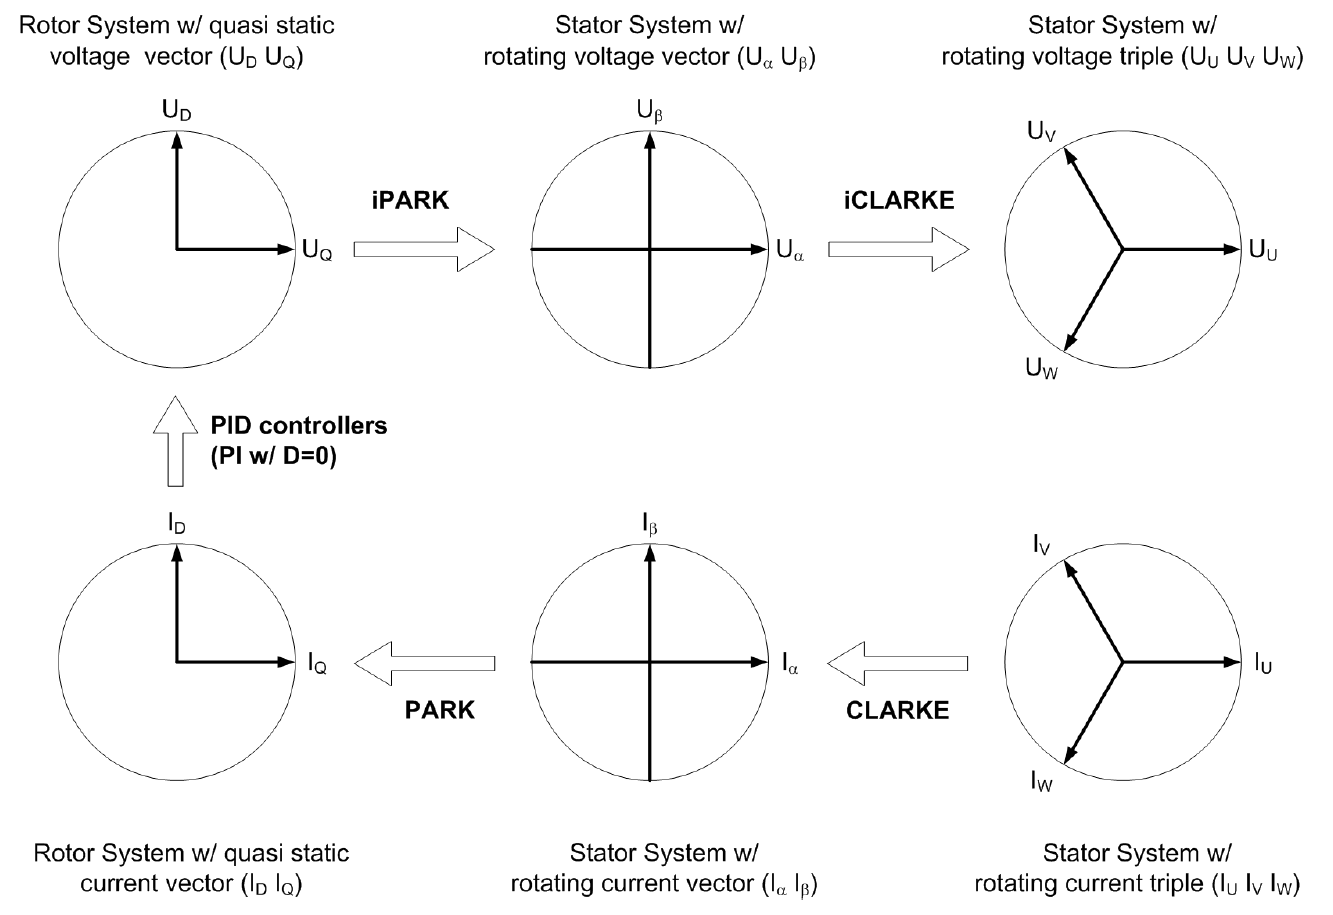
\includegraphics[width=\textwidth]{graphics/PI_Regler_Park_and_Clarke.png}
	\caption{TMC4671-EVAL Board. \cite{trinamic_datasheet_2018}}
	\label{fig:TMC4671_EVAL_Board_Park_and_Clarke}
\end{figure}

Die Clarke-Transformation (CLARKE) bildet drei Motorphasenströme ($I_{U}$,$I_{V}$,$I_{W}$) auf ein zweidimensionales
Koordinatensystem mit zwei Strömen ($I_\alpha$,$I_\beta$) ab. Basierend auf dem tatsächlichen Rotorwinkel, der durch einen Encoder oder über eine sensorlose Elektronik ermittelt wird, bildet die Park-Transformation (PARK) diese beiden Ströme auf ein näherungsweise statisches
Koordinatensystem mit zwei Strömen ($I_Q$,$I_D$) ab. Der aktuelle Strom $I_D$ steht für den Flux und der aktuelle Strom $I_Q$ für das Drehmoment. Der Flux zieht nur am Rotor, beeinflusst aber das Drehmoment nicht. Das Drehmoment wird durch den Strom $I_Q$ beeinflusst.
Zwei PI Regler ($PID_Q$, $PID_D$)\footnote{siehe Paragraph ``PID-Regler``} ermitteln zwei Spannungen ($U_Q$,$U_D$), um die gewünschten Ströme für ein Soll-Drehmoment und -Flux zu errechnen. Die ermittelten Spannungen ($U_Q$,$U_D$) werden durch die inverse Park-Transformation (iPARK) gebildet. Die inverse Clarke-Transformation (iCLARKE) transformiert diese beiden Spannungen in drei Spannungen ($U_{U}$,$U_{V}$,$U_{W}$). \cite{trinamic_datasheet_2018}

Diese drei Spannungen sind der Eingang der PWM-Engine. Dies ist in Abbildung \ref{fig:Blockdiagramm_TMC4671} und Abbildung \ref{fig:Blockdiagramm_TMC4671_PID} zu erkennen.

Für die Cocktailmaschine ist der Teil mit den PID-Reglern interessant, da wir an dieser Stelle das Verhalten des Motors regeln können. Insbesondere die Geschwindigkeit und Beschleunigung muss unter Kontrolle sein. Die Funktion der Regler wird deshalb genauer betrachtet. 

\newpage

\subsubsection{PID-Regler}

Im Folgenden wird erklärt, wie die PID-Regler im Treiber funktionieren.
In Abbildung \ref{fig:Blockdiagramm_TMC4671_PID} ist zu erkennen, dass an jeder Stelle, an der Regler verfügbar sind, $PID_n$ steht.

\begin{tabular}{lll}
$PID_x$ & = & Regler für die Position x\\
$PID_v$ & = & Regler für die Geschwindigkeit v \\
$PID_Q$ & = & Regler für den tangentialen Strom $I_Q$ \\
$PID_D$ & = & Regler für den radialen Strom $I_D$ \\
\end{tabular}

\begin{figure}[h!]
	\centering
	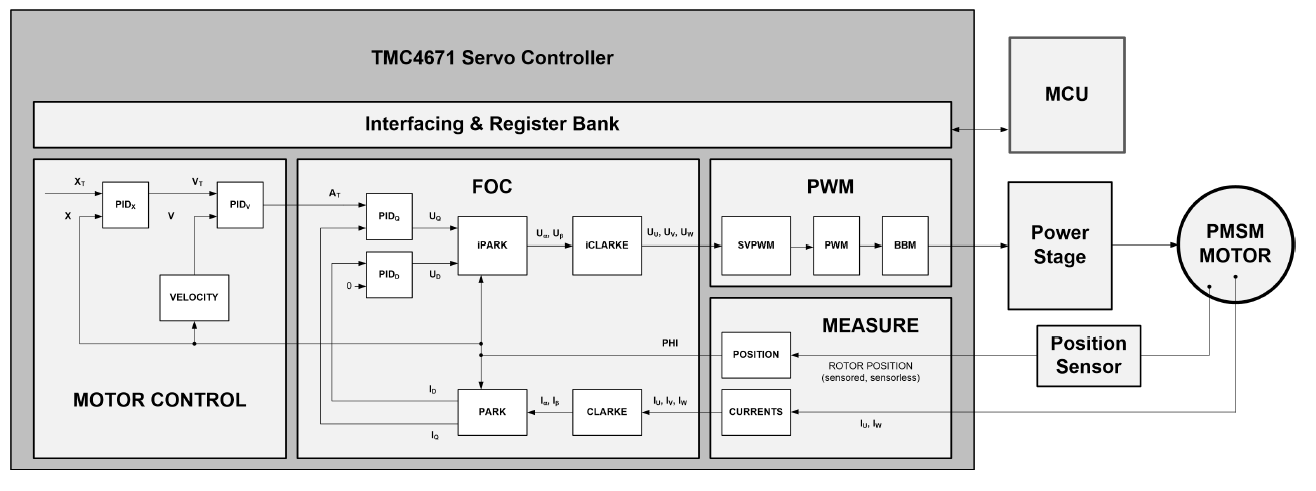
\includegraphics[width=\textwidth]{graphics/Blockdiagramm_TMC4671_FOC.png}
	\caption{Hardware FOC Blockdiagramm.\cite{trinamic_datasheet_2018}}
	\label{fig:Blockdiagramm_TMC4671_PID}
\end{figure}

 Ein DC-Motor wird vom Prinzip her wie in Abbildung \ref{fig:Blockdiagramm_TMC4671_PID_0} geregelt. Diese Abbildung zeigt einen vereinfachten Aufbau einer Antriebsregelung. Mittels den eingestellten PI-Parametern und dem eingestellten Betriebsmodus (Torque/Flux, Velocity, Position) werden beim TMC4671 die Abhängigkeiten der Regler geändert. Dies ist in Abbildung \ref{fig:Blockdiagramm_TMC4671_PID_1} ersichtlich. Im Drehmoment-Modus wird ``TARGET\_TORQUE`` als Ziel-Drehmoment verwendet. Im Geschwindigkeitsmodus wird das Zieldrehmoment vom Geschwindigkeits-PID-Regler vorgegeben. Im Drehmomentregler kann das maximale Drehmoment vorgegeben werden, welches auf den Motor gegeben wird. Eine detaillierte Übersicht der einzelnen Regler und deren Abhängigkeiten ist in Abbildung \ref{fig:Blockdiagramm_TMC4671_PID_2} zu finden.
\\

\begin{figure}[h!]
	\centering
	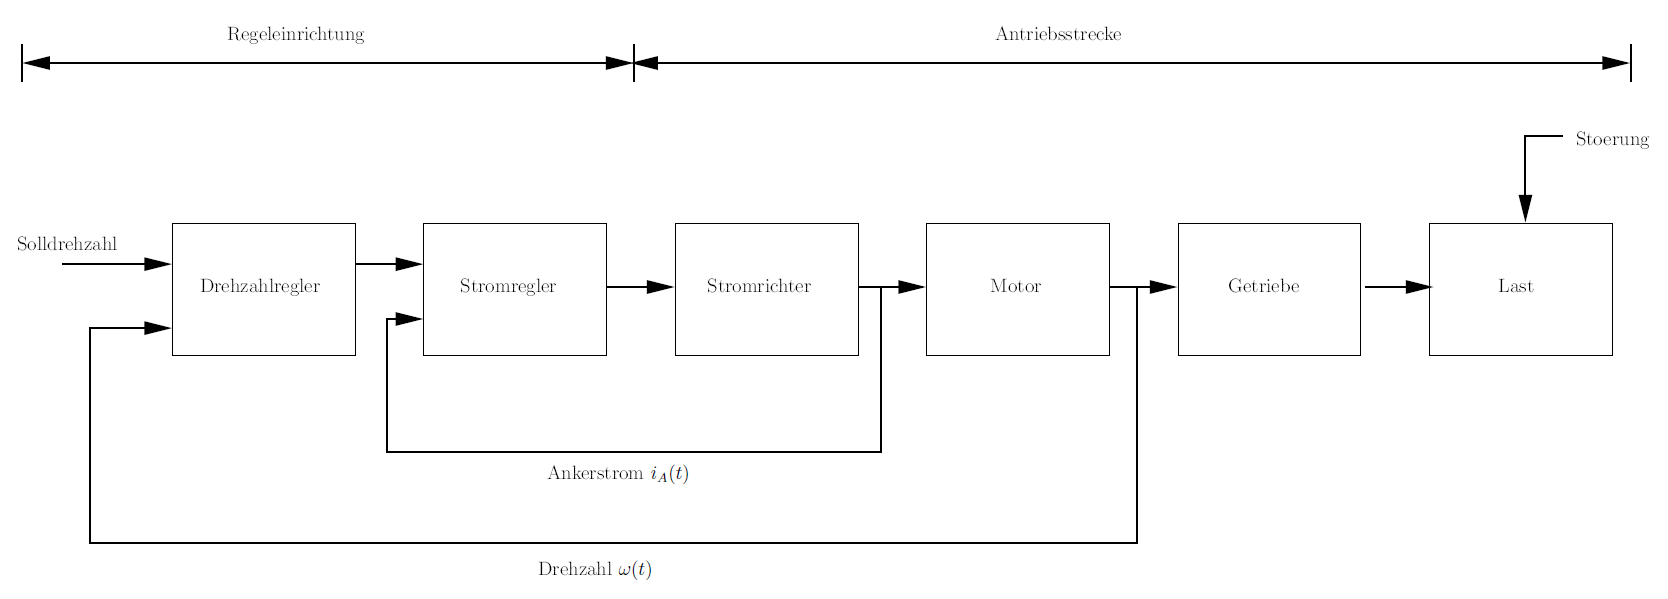
\includegraphics[width=\textwidth]{graphics/Prinzipieller_Antrieb_DC_Motor.png}
	\caption{Der Prinzipielle Aufbau einer Antriebsregelung für einen DC-Motor. 
	\cite{prof_dr-ing_raisch_stromregelung_nodate}
	}
	\label{fig:Blockdiagramm_TMC4671_PID_0}
\end{figure}

\begin{figure}[h!]
	\centering
	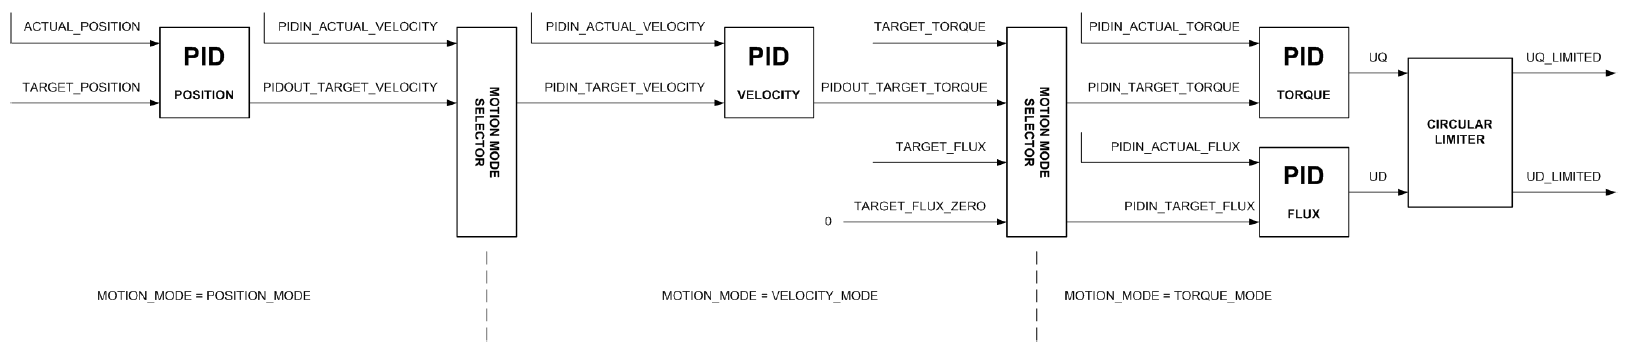
\includegraphics[width=\textwidth]{graphics/PI_Regler_Struktur_Gesamt.png}
	\caption{Abhängigkeiten der Regler.\cite{trinamic_datasheet_2018}}
	\label{fig:Blockdiagramm_TMC4671_PID_1}
\end{figure}

\newpage

\begin{figure}[h!]
	\centering
	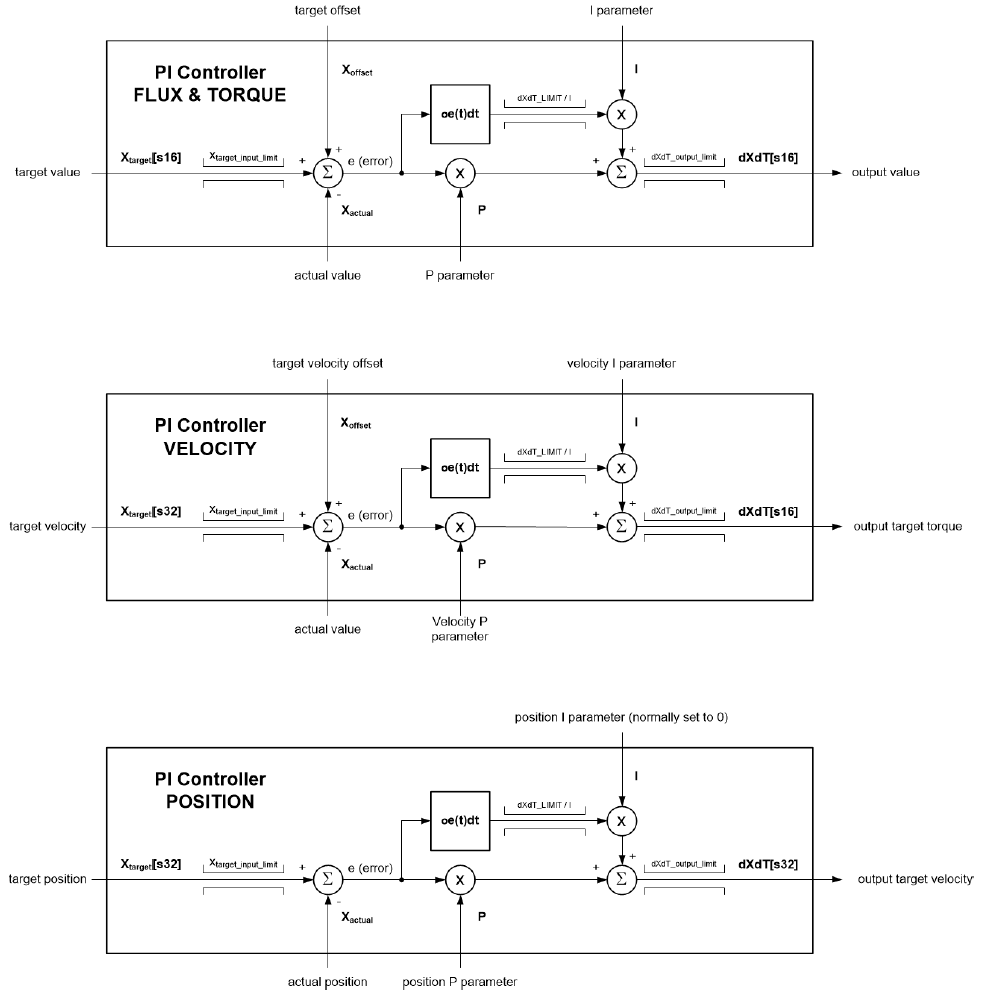
\includegraphics[width=\textwidth]{graphics/PI_Regler_Struktur.png}
	\caption{Die Reglerstufen im Detail. \cite{trinamic_datasheet_2018}}
	\label{fig:Blockdiagramm_TMC4671_PID_2}
\end{figure}

\newpage

Abbildung \ref{fig:PID_Target} zeigt, wie die Regelung im Positionsmodus eine Ziel-Position vorgibt (rot) und wie die aktuelle, gemessene Position tatsächlich ist (blau). Zu erkennen ist, dass die blaue Linie die Zielposition ziemlich steil anfährt und nicht überschiesst.

\begin{figure}[h!]
	\centering
	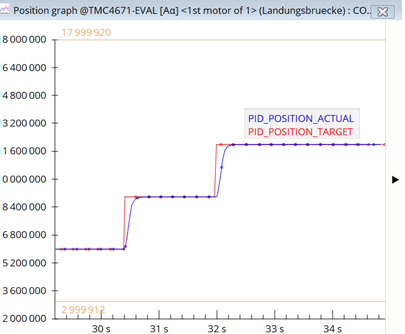
\includegraphics[width=0.6\textwidth]{graphics/PID_Target.png}
	\caption{Geschwindigkeitsregler mit Zielgraph und aktueller Graph. \cite{usb_von_herr_schleuniger_foc-motorenansteuerung_2019}}
	\label{fig:PID_Target}
\end{figure}
%\paragraph{Funktionsprinzip}\mbox{}\\

%In Abbildung \ref{fig:Blockdiagramm_TMC4671} ist ein vereinfachtes Block-Diagramm zu sehen, worin zu erkennen ist, wie die einzelnen Systemkomponenten zusammenhängen.


.
%\begin{tabbing}

%\parbox[t]{.1\textwidth}{

%MCU

%} \=\parbox[t]{.9\textwidth}{

%Kommuniziert über SPI mit dem Treiber. Die MCU schreibt und liest die Register des TMC4671. Dieser Teil wird auf dem EVAL-Board von der Landebrücke dargestellt. Bei der Cocktailmaschine wird dies der Atmega2560 sein.
%\\
%}\\

%\parbox[t]{.15\textwidth}{

%SPI

%} \> \parbox[t]{.9\textwidth}{

%Kommunikations-Interface des TMC4671. Der Treiber fungiert als Slave und decodiert die über die SPI-Schnittstelle übertragenen Daten.
%\\
%}\\

%\parbox[t]{.1\textwidth}{

%Registers

%} \>\parbox[t]{.9\textwidth}{

%Hier sind die Registerdaten gespeichert. Sie dienen dem Treiber als Parameter für dessen Funktion. Trinamic hat folgende Gruppierung festgelegt:

%\begin{multicols}{3}
%\begin{itemize}
%\item Informationen
%\item Allgemein
%\item ADC's
%\item Inputs/Outputs
%\item PWM
%\item Decoder ABN
%\item Hall digital
%\item Decoder analog
%\item PID-Regler
%\end{itemize}
%\end{multicols}

%}\\
%\parbox[t]{.15\textwidth}{
%FOC23
%} \>\parbox[t]{.9\textwidth}{
%Die FOC23-Engine führt den inneren Stromregelkreis für den Drehmomentstrom $I_Q$ und den Fluss-Strom $I_D$, einschließlich der erforderlichen Transformationen, welche noch erklärt werden. Programmierbare Begrenzer sorgen für einen sicheren Betrieb.
%\\
%}\\
%\parbox[t]{.15\textwidth}{
%Servo
%} \>\parbox[t]{.9\textwidth}{
%Mit 
%}\\
%\parbox[t]{.15\textwidth}{
%PWM
%} \>\parbox[t]{.9\textwidth}{
%Stellt Impulse für H-Brücke zur Verfügung.
%\\
%}\\
%\parbox[t]{.15\textwidth}{
%ADC
%} \>\parbox[t]{.9\textwidth}{
%Erlaubt analoge signale zu interpretieren
%}\\
%\parbox[t]{.15\textwidth}{
%Encoder
%} \>\parbox[t]{.9\textwidth}{
%Erlaubt, die Position des Rotors zu bestimmen
%}\\
%\parbox[t]{.15\textwidth}{
%Gate
%} \>\parbox[t]{.9\textwidth}{
%Steuert die Gates der Power-Stufe
%}\\
%\parbox[t]{.15\textwidth}{
%Power
%} \>\parbox[t]{.9\textwidth}{
%H-Brücke, wo der Motor angeschlossen wird.
%}\\
%\parbox[t]{.25\textwidth}{
%Current
%} \>\parbox[t]{.9\textwidth}{
%Feedback für Strom durch die Spule.
%}\\
%\parbox[t]{.25\textwidth}{
%BLDC
%} \>\parbox[t]{.9\textwidth}{
%Motor
%}\\
%\parbox[t]{.25\textwidth}{
%Encoder
%} \>\parbox[t]{.9\textwidth}{
%Resolver/ABN-Encoder
%}
%\end{tabbing}

\subsection{Förderband}
\label{subsubsec:Foerderband}

Da gemäss Kapitel \ref{subsec:Entscheidungfindung_des_Aufbaus} ein Förderband eingesetzt wird um das Glas zu bewegen, muss ein Motor eingesetzt werden, welcher das Glas mitsamt Inhalt transportieren kann. Ausserdem sollen die verschiedenen Anfahrtspositionen exakt angefahren werden können. 

\subsubsection{Anforderungen}\label{par:Anforderungen_Foerderband}

\begin{tabularx}{\textwidth}{lllX}
Mechanischer Aufbau & : & Länge & $80\pm10cm$ (Unter Annahme 10cm pro Flasche)\\
 & & Geschwindigkeit & 180cm pro 30s = 6cm/sek \\
 & & Belastbarkeit & 9.81N (1kg) \\
 & & Oberfläche & Rutschfest \\
 & & Führung & zwei Führungsstangen um den Schlitten zu bewegen. \\
 & & Schlitten & evt. 3D Druck \\
\end{tabularx}

\subsubsection{Verwendeter Aufbau}\label{par:Verwendeter_Aufbau}

Der Aufbau der Cocktailmaschine soll gemäss der Entscheidungsfindung des Aufbaus der Cocktailmaschine \ref{subsec:Entscheidungfindung_des_Aufbaus} ähnlich aussehen, wie bei der CocktailAvenue \ref{subsubsec:Aufbau_CocktailAvenue}. Allerdings sollen die Getränkebehälter nicht sichtbar hinter der Maschine platziert werden. Somit könnte man sagen, dass es eine Mischung aus der CocktailAvenue \ref{subsubsec:Aufbau_CocktailAvenue} und dem Cocktailmixer \ref{subsubsec:Aufbau_Der_Cocktailmixer} sein wird. Ein erster Prototyp soll zuerst aus Holz angefertigt werden, bevor die Maschine dann aus Metall (vorzugsweise Chromstahl) aufgebaut wird.

\subsection{Pumpen}
\label{subsubsec:Pumpen}

Um die Flüssigkeit aus den Flaschen in das Glas abzufüllen, werden gemäss Kapitel \ref{subsec:Entscheidungfindung_des_Aufbaus} Pumpen eingesetzt. Es werden daher verschiedene Typen miteinander verglichen.

\subsubsection{Anforderungen}\label{par:Anforderungen_Pumpen}

\begin{tabularx}{\textwidth}{lllX}
Durchflussmenge & : & Aus Pflichtziel & min. 0.6l pro Minute\\
 & & Aus Wunschziel & min 1.2l pro Minute \\
Spannung & : & Spannungsversorgung & 12-24V \\
Schlauchanschluss & : & Innendurchmesser & 6-8mm \\
Sonstiges & : & Hygieneanforderungen & Lebensmittelpumpe \\
\end{tabularx}

\subsubsection{Mögliche Pumpen}\label{par:Mögliche_Pumpen}

Da es sich um Lebensmittel handelt welche befördert werden sollen, werden zwei verschiedene Pumpentypen verglichen. Einerseits ist dies die Schlauchpumpe, welche über ihren mechanischen Aufbau ein Vakuum erzeugt, und somit Flüssigkeit ansaugt. Der grosse Vorteil dieses Pumpentyps ist, dass diese durch den Aufbau in der Lage ist, die zu befördernde Menge zu dosieren. In Abbildung \ref{fig:Schlauchpumpe} kann der Aufbau dieses Pumpentyps betrachtet werden. \cite{acky69_schlauchpumpe_2018}

\begin{figure}[h!]
	\centering
	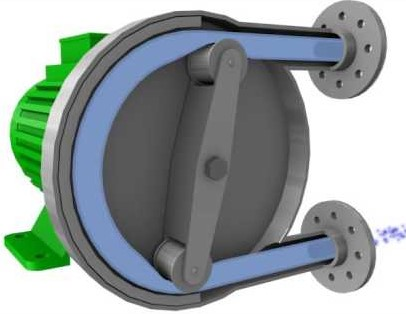
\includegraphics[width=0.6\textwidth]{graphics/Schlauchpumpe.jpg}
	\caption{Aufbau einer Schlauchpumpe \cite{creative_commons_techniker_2019}}
	\label{fig:Schlauchpumpe}
\end{figure}   

Bei jeder spezifizierten Umdrehung des Motors wird die im Schlauch befindliche Menge an Flüssigkeit zwischen zwei oder mehreren Rollen befördert. In Abbildung \ref{fig:Schlauchpumpe} ist dies nach jeder halben Umdrehung der Fall mit zwei Rollen. Werden mehrere Rollen verbaut, so kann diese Menge varriiert werden. Mit der Regelung der Drehzahl des Motors kann somit die  zu befördernde Flüssigkeitsmenge über die Zeit bestimmt werden. Eingesetzt werden diese Pumpen oft in der Medizinaltechnik, wo meist kleinere Mengen an Flüssigkeit befördert werden. Dabei kann mit einer Genauigkeit von weniger als 1\% gerechnet werden. Werden grössere Flussraten benötigt, so steigt die Ungenauigkeit dieses Pumpentyps. So muss bei einer Flussrate von 800 ml/min mit einer Abweichung von $\pm$ 8\% gerechnet werden. Um diese Ungenauigkeit beheben zu können, müsste ein externes Durchflussmessgerät installiert werden. \cite{acky69_schlauchpumpe_2018}  

Beim zweiten Pumpentyp handelt es sich um einen weiteren Typ einer Vakuumpumpe, genauer gesagt eine Membranpumpe. Bei diesem Pumpentyp wird mittels Rotation über Gummimembranen ein Vakuum erzeugt, welches das zu befördernde Medium über ein Einwegventil einsaugt und über ein weiteres Einwegventil wieder abgibt. Eine solche Pumpe ist in Abbildung \ref{fig:Membranpumpe} zu sehen. \cite{jens_uber_die_felder_membranpumpe_2019}

\begin{figure}[h!]
	\centering
	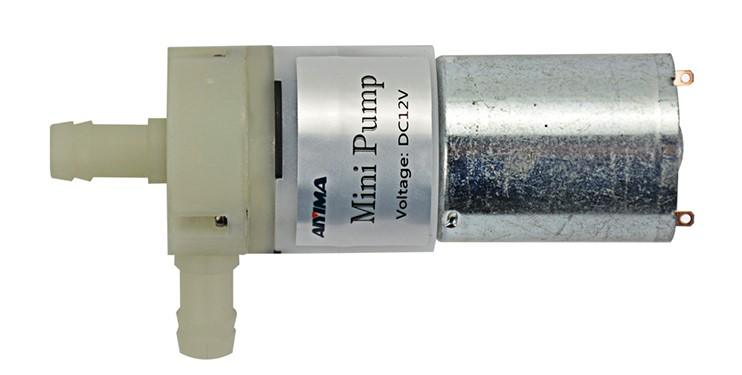
\includegraphics[width=0.6\textwidth]{graphics/Membranpumpe.jpg}
	\caption{Ansichtbild einer Membranpumpepumpe \cite{aiyimaindustrial_store_us_nodate}}
	\label{fig:Membranpumpe}
\end{figure}  

Der grosse Vorteil dieses Pumpentyps ist die hohe Lebensdauer sowie der geringe Preis. Auch bei diesem Pumpentyp kann mittels Drehzahl über die Zeit die zu befördernde Menge berechnet werden. Dies weist jedoch auch nicht die erforderliche Genauigkeit gemäss dem Pflichtenheft auf. Desshalb muss auch bei diesem Pumpentyp eine externe Durchflussmessung durchgeführt werden. \cite{jens_uber_die_felder_membranpumpe_2019}\\

\begin{table}[h!]
\begin{tabularx}{\textwidth}{|X|X|}
\hline
\textbf{Schlauchpumpe:} & \textbf{Membranpumpe:}
\\
\hline
- Spannung: 24V & - Spannung: 12V \\

- Sromverbrauch: ca. 700mA & - Sromverbrauch: <600mA\\

- Durchfluss: bis 800ml/min & - Durchfluss: 1000-1500ml/min\\

- Messung des Durchflusses: extern & - Messung des Durchflusses: extern\\

- Preis der verglichenen Pumpe: 70.86\$  & - Preis der verglichenen Pumpe: 6.37\$\\

- Bestellseite: Aliexpress & - Bestellseite: Aliexpress\\

\hline
\end{tabularx}
\caption{Vergleich der zwei Pumpentypen \cite{aiyimaindustrial_store_us_nodate}\cite{dongguan_honlite_industrial_co._ltd._800_nodate}}
\end{table}

\subsubsection{Verwendete Pumpe}\label{par:Verwendete_Pumpe}

Beide Pumpen entsprechen mindestens den Wunschzielen gemäss dem Pflichtenheft. Allerdings ist die mechanische Abnutzung beider Pumpentypen verschieden. So wird bei der Schlauchpumpe der Schlauch relativ stark beansprucht, was zur Folge hat, dass dieser mit der Zeit ausgewechselt werden muss. Die Membranpumpe hingegen bietet da eine höhere Lebensdauer. Der grösste Unterschied bietet jedoch der Preis. Da die Schlauchpumpe mehr als 10 Mal so viel kostet, wie die Membranpumpe und davon 12stk. benötigt werden, wird die Membranpumpe eingesetzt. Ausserdem kann mit der Schlauchpumpe nur das Pflichtziel gemäss Pflichtenheft umgesetzt werden und mit der Membranpumpe auch das Wunschziel. 

\subsection{Durchflussmessung}
\label{subsec:Durchflussmessung}

Da gemäss Kapitel \ref{subsubsec:Pumpen} Pumpen eingesetzt werden, welche nicht über eine integrierte Durchflussmessung verfügen, muss diese extern gemessen werden. Dies wird mittels Durchflusssensoren umgesetzt. Dazu werden verschiedene Möglichkeiten verglichen.

\subsubsection{Anforderungen}\label{par:Anforderungen_Durchflussmessung}

\begin{tabularx}{\textwidth}{lllX}
Durchflussmenge & : & Aus Pflichtziel & min. 0.6l pro Minute\\
 & & Aus Wunschziel & min 1.2l pro Minute \\
Spannung & : & Spannungsversorgung & 3.3V bis 5V \\
Schlauchanschluss & : & Innendurchmesser & 6-8mm \\
Sonstiges & : & Hygieneanforderungen & Lebensmittelsensor \\
\end{tabularx}

Es existieren viele verschiedene Varianten um eine Durchflussmessung durchführen zu können. Dazu gehören folgende Verfahren:

\begin{itemize}
\item akustische Verfahren
\item gyroskopische Verfahren
\item magnetisch-induktive Verfahren
\item mechanisch-volumetrische Verfahren
\item optische Verfahren
\item thermische Verfahren
\item Wirkdruck-/Stauverfahren
\end{itemize}

Viele dieser Verfahren werden nur bei grösseren Durchflussmengen eingesetzt. Wieder andere werden verwendet um den Durchfluss von verschieden Medien zu bemessen. Da es sich bei diesem Projekt um relativ geringe Durchflussmengen von weniger als 2l/min handelt eignet sich ein mechanisch-volumetrisches Verfahren am besten. \cite{alfaomega_durchflussmesser_2019}

\subsubsection{Verwendeter Durchflusssensor}\label{par:Verwendter_Durchflussssensor}

Beim verwendeten Durchflussmessgerät handelt es sich um ein sogenannten Flügelradzähler von Sea gemäss Abbildung \ref{fig:Flügelradzähler}. Dies ist ein hermetisch abgeschlossener Durchflussgeber, dessen Kernstück aus einem Flügelrad besteht. Bei Durchfluss wird dieses Flügelrad in Bewegung gesetzt, welches über einen Hallsensor elektronische Impulse erzeugt. Somit kann die durchfliessende Menge elektronisch bestimmt werden. \cite{five_+_tools_store_us_nodate}
 
\begin{figure}[h!]
	\centering
	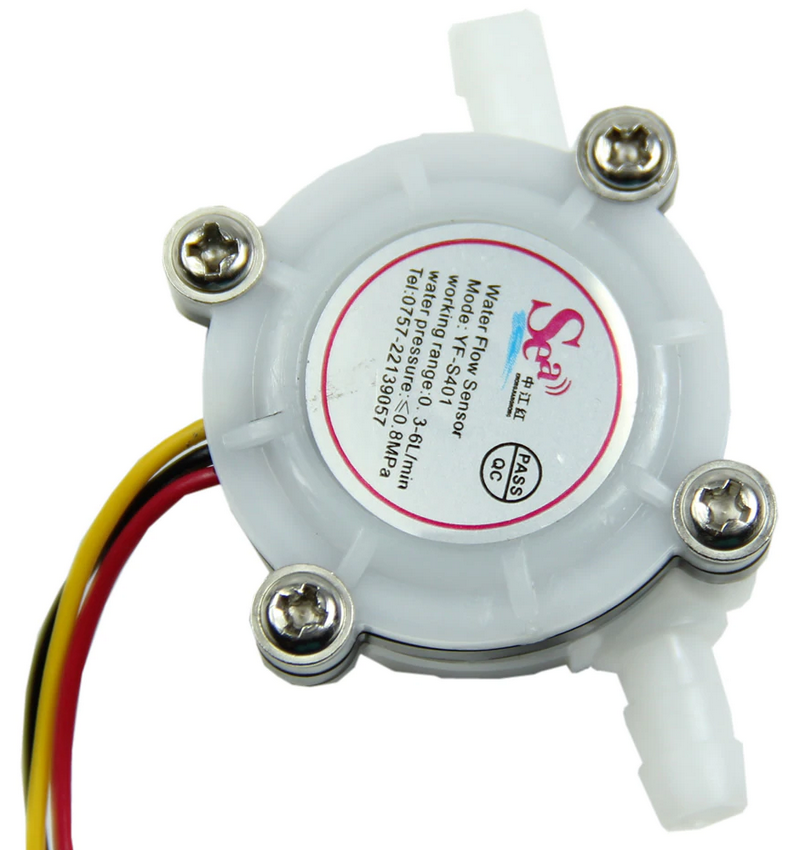
\includegraphics[width=0.6\textwidth]{graphics/Fluegelradzaehler.png}
	\caption{Sea Flügelradzähler \cite{five_+_tools_store_us_nodate}}
	\label{fig:Flügelradzähler}
\end{figure}

\begin{table}[h!]
\centering
\begin{tabularx}{\textwidth/2}{|X|}
\hline
\textbf{Technische Daten:}\\
\hline
- Spannung: 3.3 - 5V\\

- Sromverbrauch: ca. 15mA\\

- Messbarere Durchflussmenge: 0.3-6l/min\\

- Preis: 2.09 CHF \\

- Bestellseite: Aliexpress\\

\hline
\end{tabularx}
\caption{Technische Daten Sea Durchflussmessgerät \cite{five_+_tools_store_us_nodate}}
\end{table}


\newpage
\subsection{Display}
\label{subsubsec:Grobkonzept_Display}
Um die Maschine bedienen zu können, wird ein Display benötigt. Die Verwendung von Buttons soll verhindert werden. Aus diesem Grund wird ein Touch-Display implementiert.

\subsubsection{Anforderungen}\label{par:Anforderungen_Display}

%\begin{tabbing}
%\parbox[t]{.25\textwidth}{
%Kommunikation
%} \= \parbox[t]{.75\textwidth}{
%UART oder SPI\\
%}\\
%\parbox[t]{.25\textwidth}{
%Spannung
%} 
%\>\parbox[t]{.75\textwidth}{
%5V oder 3.3V\\
%}\\
%\parbox[t]{.25\textwidth}{
%Bedienung
%} 
%\>\parbox[t]{.75\textwidth}{
%Touch-Panel\\
%}\\
%\parbox[t]{.25\textwidth}{
%Grösse
%}
%\>\parbox[t]{.75\textwidth}{
%$\pm$ 10cm Diagonale\\
%}\\
%\parbox[t]{.25\textwidth}{
%Sonstiges
%}
%\>\parbox[t]{.75\textwidth}{
%Hintergrundbeleuchtung, eigebauter SD-Kartenslot vorteilhaft.\\
%}
%\end{tabbing}
\begin{tabular}{lll}
Kommunikation & : & UART oder SPI\\
Spannung & : & 5V oder 3.3V \\
Bedienung & : & Touch-Panel \\
Grösse & : & $\pm$ 10cm Diagonale \\
Sonstiges & : & Hintergrundbeleuchtung, eingebauter SD-Kartenslot vorteilhaft \\
\end{tabular}

%\begin{itemize}
%\item Kommunikation
%\begin{itemize}
%\item SPI
%\item UART
%\end{itemize}
%\item Spannung
%\begin{itemize}
%\item Versorgungsspannung: 5V
%\item Versorgungsspannung: 3.3V
%\end{itemize}
%\item Bedienung
%\begin{itemize}
%\item Touch-Display (resistiv)
%\end{itemize}
%\item Grösse
%\begin{itemize}
%\item $\pm$ 10cm
%\end{itemize}
%\item Sonstiges
%\begin{itemize}
%\item Hintergrundbeleuchtung
%\item SD-Karte vorteilhaft
%\end{itemize}
%\end{itemize}

\subsubsection{In Frage kommende Displays}\label{par:In_Frage_kommendes_Display}

Folgende Displays kommen gemäss den Anforderungen für die Cocktailmaschine in Frage:

\begin{tabular*}{\textwidth}{@{\extracolsep{\fill}}|c|c|c|c|c|}\hline
	\textbf{Displaynr.} & \textbf{Hersteller} & \textbf{Herstellernr.} & \textbf{Vertrieb} & \textbf{Kosten} \\ \hline
    1 & Geekcreit® & TFT Touch Display & Banggood & CHF 12.78 \\\hline
    2 & 4D Systems & 4DLCD-28320240-RTP & Mouser &CHF 18.76 \\ \hline
    3 & 4D Systems & 4DLCD-35480320-RTP & Mouser & CHF 23.77 \\ \hline
    4 & Matrix Orbital & EVE2-43A-BLM-TPR & Mouser & CHF 48.04\\ \hline
    5 & Nextion & NX8048T070 & Banggood & CHF 61.44\\ \hline
\end{tabular*}

\begin{table}[h]
\begin{tabular*}{\textwidth}{@{\extracolsep{\fill}}|l|c|c|c|c|c|}
\hline
\textbf{Display} & \textbf{1} & \textbf{2} & \textbf{3} & \textbf{4} & \textbf{5} \\ \hline
Kommunikation & SPI & SPI & SPI & SPI & UART\\ \hline
Versorgungssp. & 3.3V/5V & 2.8V & 2.8V & 3.3V & 5V \\ \hline
Strom & - & 25mA & 25mA & 50mA & 510mA\\ \hline
Vertikal & 2.8" & 2.8" & 3.5" & 4.3" & 7" \\ \hline
Grösse (mm) & 78 x 53 & 50 x 69.2 & 54.5 x 83  & 105.4 x 67.1 & 154.08 x 85.92\\ \hline
Pixel & 240 x 320 & 240 x 320 & 320 x 480 & 480 x 272 & 800 x 480 \\ \hline
Touch Panel & Resistive & Resistive & Resistive & Resistive & Resistive \\ \hline
Hintergrundbel. & LED & LED & LED & LED & LED\\ \hline
SD-Karte & Ja & Nein & Nein & Nein & Ja\\ \hline
\end{tabular*}
\caption{Displays im Vergleich}
\label{tab:Vergleich_Displays}
\end{table}

\subsubsection{Verwendetes Display}\label{par:Verwendetes_Display}

Um die Cocktailmaschine bedienen zu können, wird das Nextion-Display (5) gemäss Tabelle \ref{tab:Vergleich_Displays} eingesetzt. Das Nextion-Display ist zwar das teuerste Display in der Vergleichsserie, hat jedoch zwei grosse Vorteile. Zum Einen ist dies die grosse Entwicklungsumgebung und die vorhandene Community. Für die Displays von Nextion besteht eine Software, mit welcher relativ einfach GUI's (Graphical User Interface's) erstellt werden können. Dies erleichtert den Programmieraufwand ungemein. Des Weiteren ist die Bedienung auf einem 7-Zoll Display für diesen Zweck am benutzerfreundlichsten empfunden worden. 

\subsection{Mikrocontroller}\label{subsubsec:Mikrocontroller}

Der Mikrocontroller ist dafür da, die verwendeten Bauteile gemäss Systemanforderungen anzusteuern und auszulesen. Er ist folglich dafür da, die Eingaben auf dem Display zu verarbeiten, die Getränke zu speichern und die zu bewegenden Peripherien zu steuern.

\subsubsection{Anforderungen}\label{par:Anforderungen_Mikrocontroller}

\begin{tabularx}{\textwidth}{lllX}
Flüssigkeitsbeförderung & : & Pumpen & - 12x Digital Outputs\\
 & & Durchflussmessung & - 12x Digital Inputs\\
Motorentreiber & : & Kommunikation & - SPI \\
 &  &  & - 1x Digital Output \\
 &  & Status & - 1x Digital Input \\
 &  & EN\_IN & - 1x Digital Output \\
Resolver & : & PWM 8kHz & - 1x Digital Output PWM \\
Display & : & Kommunikation & - UART \\
Computer USB & : & Kommunikation & - UART \\
\end{tabularx}

%\begin{tabbing}
%\parbox[t]{.25\textwidth}{Flüssigkeitsbeförderung} \= \parbox[t]{.25\textwidth}{Pumpen} \= \parbox[t]{.5\textwidth}{- 12x Digital Outputs Pumpen}\\
%\> \linefill \\
%\parbox[t]{.25\textwidth}{\mbox{}} \> \parbox[t]{.25\textwidth}{Durchflussmessung} \> \parbox[t]{.5\textwidth}{- 12x Analog/Digital Inputs Durchflussmessung}\\
%\linefill \\
%\parbox[t]{.25\textwidth}{Motorentreiber} \> \parbox[t]{.25\textwidth}{Kommunikation mit BLDC-Motorentreiber}
%\> \parbox[t]{.5\textwidth}{- SPI (MISO, MOSI, CLK)\newline - SPI CS\newline - UART (TXD\_SYNC1, RXD\_SYNC2)}\\
%\> \linefill \\
%\parbox[t]{.25\textwidth}{\mbox{}} \> \parbox[t]{.25\textwidth}{Sonstige Anschlüsse} \> \parbox[t]{.5\textwidth}{- Dir (Digital)\newline - Step (Digital)\newline - Status (Digital)\newline - EN\_IN (Digital)\newline - GPIO\_0 (Digital)\newline - GPIO\_1 (Digital)\newline - GPIO\_2 (Digital)\newline - GPIO\_7 (Digital)\newline - AGPI\_A (Analog, nicht umbedingt benötigt)\newline - AGPI\_B (Analog, nicht umbedingt benötigt)\newline - PWM\_IN (PWM)}\\
%\linefill \\
%\parbox[t]{.25\textwidth}{Display} \> \parbox[t]{.25\textwidth}{Kommunikation mit TFT Touch Display}\> \parbox[t]{.5\textwidth}{ - TF\_CS (Digital)\newline - TFT\_DC (Digital)\newline - TFT\_Backlight (Digital)\newline - SPI (MISO, MOSI, CLK)\newline
% - SPI CS}\\
% \> \linefill \\
%\parbox[t]{.25\textwidth}{\mbox{}} \> \parbox[t]{.25\textwidth}{Bedienung Touch Panel} \> \parbox[t]{.5\textwidth}{- Touch Panel (4x Analog)}\\
%\linefill \\
%\parbox[t]{.25\textwidth}{Bluetooth/WiFi-IC} \> \parbox[t]{.25\textwidth}{Kommunikation mit IC} \> \parbox[t]{.5\textwidth}{ - UART (TX, RX)}\\
%\end{tabbing}
\newpage
\subsubsection{Total benötigte Anschlüsse}\label{par:Anforderungen_Mikrocontroller_Zus}

Ins Gesamt sind folglich folgende Anschlüsse nötig:
\begin{itemize}
	\item 14 Digital Outputs
	\item 13 Digital Inputs
	\item 1 PWM Pin
	\item 1 SPI
	\item 3 UART
\end{itemize}

\subsubsection{In Frage kommende Mikrocontroller}\label{par:In_Frage_kommender_Mikrocontroller}

Aufgrund einer ziemlich grossen Community und damit auch weit verbreiteter Anwendungsgebieten sowie Forumtauglichkeit wurden Mikrocontroller des Herstellers Atmel untersucht. Folgende Mikrocontroller erfüllen die Mindestanforderungen an das System:

\begin{itemize}
\item Atmega 640
\item Atmega 1280
\item Atmega 2560
\end{itemize}

In der folgenden Tabelle \ref{Table:Gegenueberstellung_Mikrocontroller} sind die Eigenschaften der Mikrocontroller gegenübergestellt.

\begin{table}[ht]
\centering
\begin{tabular*}{\textwidth}{@{\extracolsep{\fill}}|l|c|c|c|}\hline
\textbf{Mikrocontroller} & ATMEGA640-16AU & ATMEGA1280-16AU & ATMEGA2560-16AU \\ 
\hline 
\textbf{Preis} & CHF 7.93 (Digikey) & CHF 10.84 (Digikey) & 12.09 (Digikey)\\ 
\hline 
\textbf{Kerngrösse} & 8-bit & 8-bit & 8-bit \\ 
\hline 
\textbf{Geschwindigkeit} & 16MHz & 16MHz & 16MHz \\ 
\hline 
\textbf{Konnektivität} & \shortstack{EBI/EMI, I2C,\\ SPI, UART} & \shortstack{EBI/EMI, I2C,\\ SPI, UART} & \shortstack{EBI/EMI, I2C,\\ SPI, UART} \\ 
\hline 
\textbf{I/O} & 86 & 86 & 86 \\ 
\hline 
\textbf{FLASH-Grösse} &  64KB & 128KB & 256KB \\ 
\hline 
\textbf{Spannung} & 2,7 bis 5,5V & 2,7 bis 5,5V & 4,5 bis 5,5V \\ 
\hline 
\textbf{Analogwandler} & 16x10b & 16x10b & 16x10b \\ 
\hline 
\textbf{Gehäuse} & 100-TQFP & 100-TQFP & 100-TQFP \\ 
\hline 
\end{tabular*}\\
\caption{Gegenüberstellung der in Frage kommenden Mikrocontroller}\label{Table:Gegenueberstellung_Mikrocontroller}
\end{table}

\subsubsection{Verwendeter Mikrocontroller}\label{par:Verwendeter_Mikrocontroller}

In der Tabelle \ref{Table:Gegenueberstellung_Mikrocontroller} ist ersichtlich, dass sich die Mikrocontroller nur in der Speichergrösse sowie Versorgungsspannung unterscheiden. Unter der Annahme, dass die Programmierung des Displays einen grossen Teil des Speichers einnimmt, wird ein Chip mit grossem FLASH-Speicher bevorzugt. Weiter besteht mit diesem Chip die Möglichkeit, mit einem Entwicklungsboard wie dem Arduino Mega, einen Prototyp des gesamten Systems zu simulieren. Deshalb wird für dieses Projekt der \textbf{\textcolor{blue}{ATMEGA2560-16AU}} verwendet.

\pagebreak
\section{Detailkonzept}
\label{sec:Detailkonzept}

Im Detailkonzept werden die einzelnen Schaltungsteile aufgezeigt und erläutert. Dabei handelt es sich und die komplette Hardware mit den dazugehörigen Schemata. Dazu zählt die Speisung, der Mikrocontroller, die Motorenansteuerung, die Pumpenansteuerung sowie die Displayansteuerung.

\subsection{Speisungen}
\label{subsec:Detailkonzept_Speisungen}

Wie dem Grobkonzept in Kapitel \ref{subsec:Blockschaltbild} entnommen werden kann, werden für das System vier verschiedene Speisungen benötigt. Es handelt sich dabei um eine 48V-, eine 12V-, eine 5V- und eine 3.3V Spannungsquelle. Auf diese Speisungen und deren Realisierung wird in den folgenden Unterkapiteln eingegangen. 

\subsubsection{48V Speisung}\label{subsubsec:48V_Speisung}

Um die benötigten 48V des Motors sicher zu stellen, wird ein fertiges Netzteil extern eingekauft. Auch alle weiteren Speisungen werden aus den 48V generiert.  Dabei muss jedoch abgeschätzt werden, wie viel Leistung dieses 48V Netzteil zur Verfügung stellen muss. Dazu wird in folgender Auflistung eine Leistungsabschätzung gemacht.

\begin{tabularx}{\textwidth}{llllllX}
 \textbf{Bauteil}& \textbf{Beschreibung} & \textbf{Referenz} & \textbf{U} & \textbf{Max. I} \\
\hline
Motor & Stillstandstrom & \cite[S.4]{sigmatec_servomotoren_2018}& 48V & I$_S$ & = & 5.41A 
\\
 & Nennstrom & \cite[S.4]{sigmatec_servomotoren_2018} & 48V & I$_N$ & = & 5.21A\\
\\
TMC6200 & Motorspannung & \cite[S.36]{trinamic_tmc6200_datasheet_2013}& 48V & I$_{V_S}$(24V) & = & 7mA \\
 & Analog Versorgung & \cite[S.36]{trinamic_tmc6200_datasheet_2013} & 12V & I$_{V_{SA}}$(24V) & = & 8mA\\
 & IC Versorgung & \cite[S.36]{trinamic_tmc6200_datasheet_2013} & 3.3V/5V & I$_{V_{CC}}$(5V) & = & 6mA\\
 & Digital Versorgung & \cite[S.36]{trinamic_tmc6200_datasheet_2013} & 3.3V/5V& I$_{V_{IO}}$(5V) & = & 30uA\\
 \\
TMC4671 & IC Versorgung & \cite[S.140]{trinamic_datasheet_2018} & 3.3V & I$_{IO}$ & = & k.A \\
 & Analog Referenz & \cite[S.141]{trinamic_datasheet_2018} & 5V & U$_{Ref}$ & = & 5V \\
\\
Resolver & TCA0372 Versorgung & \cite[S.3]{on_semiconductor_operational_2020}& 5V & I(25$^\circ C$) & = & 14mA \\
 & TCA0372 Output & & 5V & $I_{Spule}$ & = & 90mA\\
 & MC33202 & \cite[S.3]{on_semiconductor_low_2018}& 5V & I(25$^\circ C$) & = & 2.25mA \\
\\
Mikrocontroller & IC Versorgung & \cite[S.355]{atmel_8-bit_2014}& 5V & I$_{V_{max}}$ & = & 200mA \\
\\
Level-Shifter & IC Versorgung & \cite[S.3]{nxp_semiconductors_74hc4050_2016} & 3.3V & I$_{V_{max}}$ & = & 150mA\\
\\
ESP32 & IC Versorgung & \cite[S.21]{espressif_systems_esp32_2020}& 3.3V & I$_{V_{max}}$ & = & 68mA\\
\\
Display & Versorgung  & \cite{patrick_nx8048t070_nodate}& 5V & I$_{V_{max}}$ & = & 510mA\\
\\
Pumpen & Arbeitsspannung  & \cite{aiyimaindustrial_store_us_nodate}& 12V & I$_{V_{max}}$ &  = & 600mA\\
\\
Durchflusssensor & Versorgung  & \cite{five_+_tools_store_us_nodate}& 5V & I$_{V_{max}}$ &  = & 15mA\\
\\
\end{tabularx}

Die grossen Verbraucher, welche in das Gewicht fallen, sind in diesem Fall die Pumpen, das Display und der Förderbandmotor. Beim Förderbandmotor muss jedoch auch beachtet werden, dass dieser niemals unter Vollbelastung arbeiten wird. Auch bei den Pumpen wird jeweils immer nur eine arbeiten. Somit ergibt sich eine Leistung von ca. 16.44W für alle Komponenten ohne den Motor. Dies beinhaltet eine Pumpe, zwölf Durchflussmessgeräte, das Display und alle integrierten Schaltkreise. Da der Motor nie unter Vollast arbeiten wird, wird mit maximal 2A Arbeitsstrom gerechnet. Dies ergibt zusätzlich eine Leistung von 96W bei 48V. 

Um auf der sicheren Seite zu sein wird daher ein Netzteil benötigt, welches bei 48V ca. 150W Leistung liefert. Dies entspricht bei 100\% Wirkungsgrad der einzelnen Bauteile einem Ausgangsstrom von 3,125A. Eingesetzt  wird ein 48V/500W Netzteil von Aliexpress. Der Grund für diese Überdimensionierung ist, dass der Preis sich lediglich um 2CHF unterscheidet und man auf diese Weise in jedem Fall abgesichert ist. Dieses kann in Abbildung \ref{fig:Netzteil48V} begutachtet werden. \cite{aliexpress_us_nodate}.

\begin{figure}[h!]
	\centering
	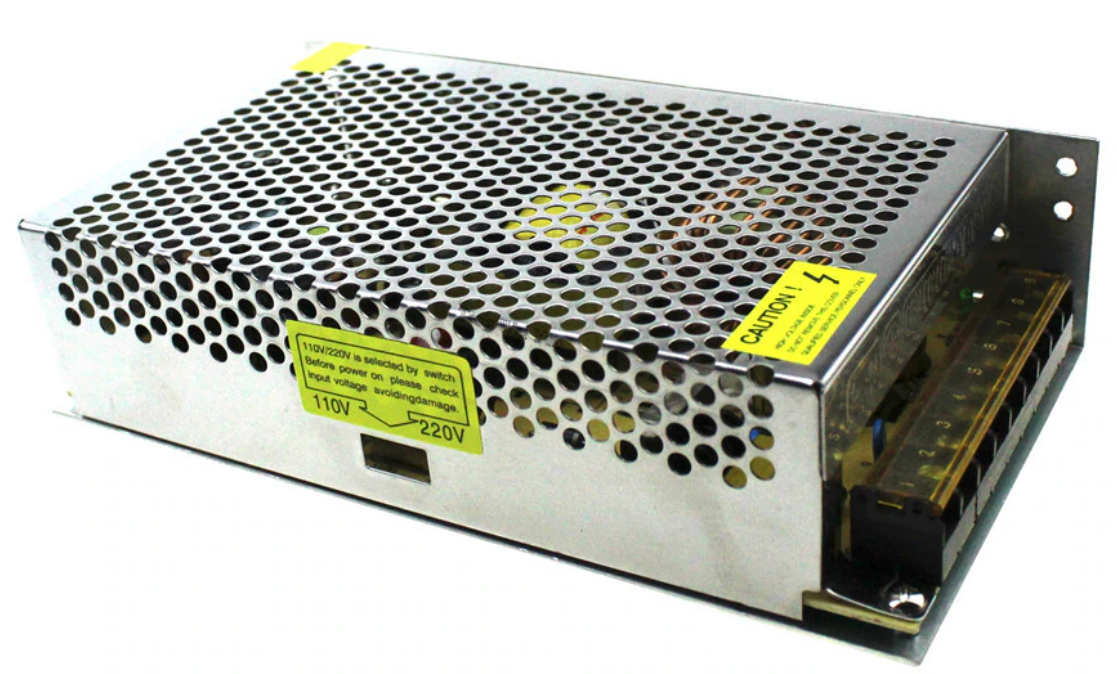
\includegraphics[width=0.8\textwidth]{graphics/Netzteil48V.png}
	\caption{Ansichtsbild des 48V Netzteils \cite{aliexpress_us_nodate}.}
	\label{fig:Netzteil48V}
\end{figure} 

\subsubsection{12V Speisung}\label{subsubsec:12V_Speisung}

Die 12V Speisung wird mittels Schaltspannungsregler realisiert. Es handelt sich hierbei um einen Regler von Monolithic Power Systems. Genauer gesagt um den MP24943DN-LF. Die Auswahl ist auf dieses Bauteil gefallen, da eine relativ hohe Eingangsspannung von 48V verarbeitet werden muss. Der MP24943DN-LF kann am Eingang mit Spannungen von 4.5-55V arbeiten und dabei eine Ausgangsspannung von 0.8-45V erzeugen. Dies bei einem maximalen Strom von bis zu 3A. Die Realisierung der 12V Speisung kann in Abbildung \ref{fig:12VSpeisung_Schema} betrachtet werden. \cite{mouser_mp24943dn-lf_nodate}

\begin{figure}[h!]
	\centering
	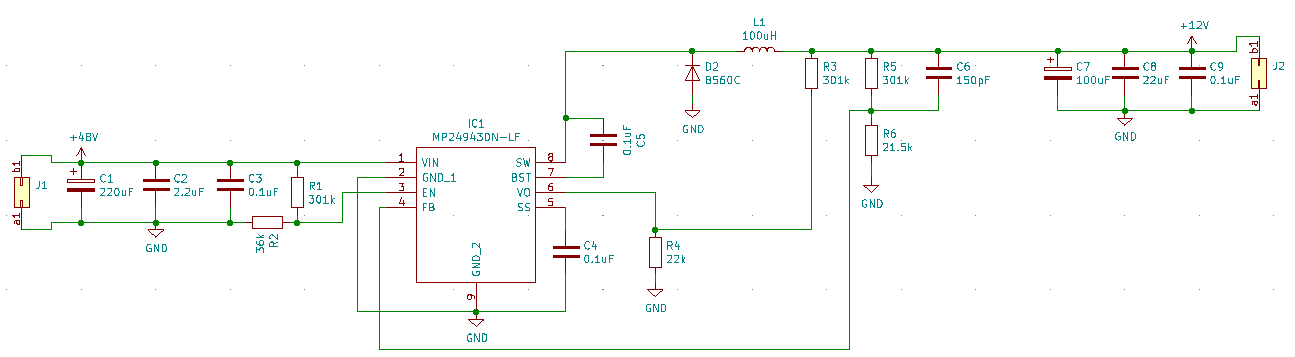
\includegraphics[width=\textwidth]{graphics/12V_Speisung_Schema.png}
	\caption{Schema der 12V Speisung}
	\label{fig:12VSpeisung_Schema}
\end{figure}  
\newpage
Bei den Kondensatoren C1-C3 handelt es sich um Filterkondensatoren, welche hochfrequente Störungen der Eingangsspannung von 48V glätten. Der Enable Eingang wird mit dem Spannungsteiler R1 \& R2 auf aktiv gesetzt. \cite{mouser_mp24943dn-lf_nodate}  

Die gewünschte Ausgangsspannung wird mittels Spannungsteiler R5 \& R6 eingestellt, welche auf den Feedback Eingang rückgekoppelt werden. Diese berechnet sich laut Datenblatt gemäss Formel \ref{equ:Ausgangsspannung_12V}. \cite{mouser_mp24943dn-lf_nodate}

\begin{align}
R6 &= \frac{R5}{\frac{Vout}{0.8}-1}
\label{equ:Ausgangsspannung_12V}
\end{align}

Bei einem Widerstandsverhältnis von R5=301k$\Omega$ \& R6=21.5k$\Omega$ entspricht dies einer Ausgangsspannung von 12V.

Um einer Überspannung vorbeugen zu können, wird am Eingang VO ein Spannungsteiler implementiert. Diese wird am VO-Eingang mit einer Referenzspannung von 0.9V verglichen. Übersteigt die Spannung an VO die Referenzspannung von 0.9V, so wird der Regler ausgeschaltet, bis die Spannung wieder unter 0.9V fällt. Als maximale Ausgangsspannung wurde hierbei eine Spannung von 13V gewählt. Diese Wahl wurde getroffen, da die 12V ausschliesslich für die Ansteuerung der Pumpen verwendet wird und diese eine Spannung von 13V verkraften können ohne Schaden zu nehmen. Der Spannungsteiler wird gemäss Datenblatt mit der Formel \ref{equ:Vovp_12V} berechnet. \cite{mouser_mp24943dn-lf_nodate}

\begin{align}
R4 &= \frac{R3}{\frac{Vovp}{Vovref}-1}
\label{equ:Vovp_12V}
\end{align}

Bei einem Widerstandsverhältnis von R3=301k$\Omega$ \& R4=22k$\Omega$ entspricht dies einer Überspannungsschutzschwelle von 13.21V. \cite{mouser_mp24943dn-lf_nodate}

Der Rippel des Spulenstroms lässt sich gemäss Formel \ref{equ:12V_Spulenberechnung} berechnen. Dieser sollte gemäss Datenblatt ca. 30\% des maximalen Ausgangsstroms von 3A betragen. \cite{mouser_mp24943dn-lf_nodate} 

\begin{align}
L1 &= \frac{Vout*(Vin-Vout)}{Vin*\Delta IL*fosc}
\label{equ:12V_Spulenberechnung}
\end{align}

Der interne Oszillator läuft dabei bei einer Frequenz von 100kHz. Bei der ausgewählten Spule von 100$\mu$H erhalten wir ein $\Delta$I$_{L}$ von 0.9A. Ausserdem wird im Datenblatt darauf hingewiesen, dass die gewählte Spule auf mindestens 125\% des maximalen Ausgangsstroms von 3A ausgelegt werden soll. Auch der Gleichstromwiederstand der Spule sollte $ \leq \ $ 200m$\Omega$  sein. \cite{mouser_mp24943dn-lf_nodate}

Mit den Kondensatoren C7, C8 \&C9 wird die Ausgangsspannung zum Abschluss noch geglättet. Bei den Eingangskondensatoren, sowie den Ausgangskondensatoren sollte es sich um low ESR Typen handeln. \cite{mouser_mp24943dn-lf_nodate}

\subsubsection{5V Speisung}
\label{subsubsec:5V_Speisung}

Bei der 5V Speisung wurde erneut auf den MP24943DN-LF von Monolithic Power Systems gesetzt. Die Beschaltung ist dabei die gleiche, wie bei der 12V Speisung. Der Unterschied ist jedoch, dass für die Ausgangsspannung und für die Überspannungsschwelle andere Widerstandsverhältnisse gewählt werden müssen. Auch die Spule muss anders ausgelegt werden. In Abbildung \ref{fig:5VSpeisung_Schema} ist das Schema der 5V Speisung zu sehen. \cite{mouser_mp24943dn-lf_nodate} 
 
\begin{figure}[h!]
\centering
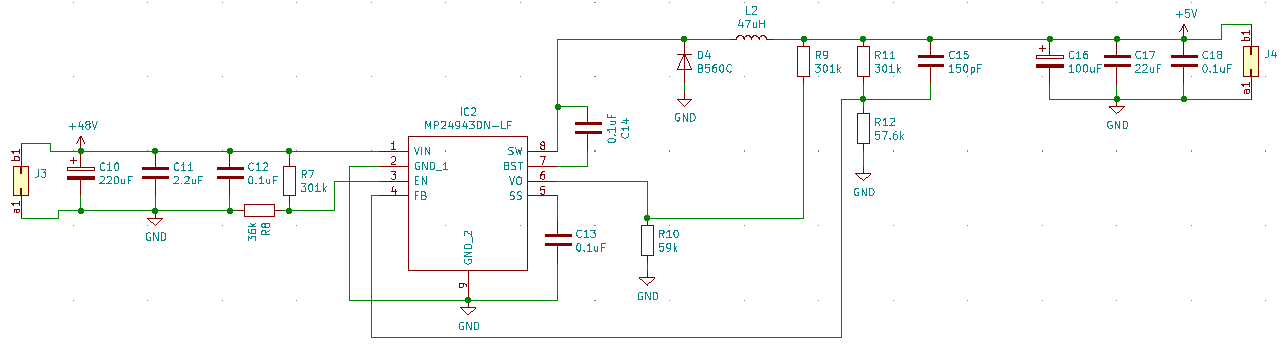
\includegraphics[width=\textwidth]{graphics/5V_Speisung_Schema.png}
\caption{Schema der 5V Speisung}
\label{fig:5VSpeisung_Schema}
\end{figure} 
 
Das Widerstandsverhältnis von R11 \& R12, welches die Ausgangsspannung definiert, wurde gemäss Formel \ref{equ:Ausgangsspannung_12V} berechnet. Somit ergeben sich für R11=301k$\Omega$ und für R12=57.6k$\Omega$, Was einer Ausgangsspannung von 4.98V entspricht. \cite{mouser_mp24943dn-lf_nodate}

Beim Überspannungsschutz muss darauf geachtet werden, dass der Mikrokontroller AtMega2560-16AU nur in einem Spannungsbereich von 4.5V-5.5V betrieben werden darf. Die maximal verträgliche Eingangsspannung liegt laut Datenblatt bei 6V. Somit muss der Überspannungsschutz so gestaltet werden, dass die Schwelle von 6V nicht überschritten werden kann. Um dies erreichen zu können, wurde für R9=301k$\Omega$ und R10=53k$\Omega$ gewählt. Gemäss Formel \ref{equ:Vovp_12V} erhält man so eine Überspannungsschutzschwelle von 6V. \cite{mouser_mp24943dn-lf_nodate}

Der interne Oszillator läuft wiederum bei einer Frequenz von 100kHz. Bei der ausgewählten Spule von 47$\mu$H erhalten wir ein $\Delta$I$_{L}$ von 0.953A. Auch hier gilt gemäss Datenblatt, dass die gewählte Spule auf mindestens 125\% des maximalen Ausgangsstroms von 3A ausgelegt werden soll. Auch der Gleichstromwiederstand der Spule sollte $ \leq \ $ 200m$\Omega$  sein. \cite{mouser_mp24943dn-lf_nodate} 

Mit den Kondensatoren C16, C17 \&C18 wird die Ausgangsspannung zum Abschluss noch geglättet. Bei den Eingangskondensatoren, sowie den Ausgangskondensatoren sollte es sich um low ESR Typen handeln. \cite{mouser_mp24943dn-lf_nodate}
\newpage
\subsubsection{3,3V Speisung}
\label{subsubsec:3,3V_Speisung}

Um die Treiber der Motorenansteuerung ansteuern zu können, wird zusätzlich eine 3,3V Speisung verbaut. Diese muss gemäss der Leistungsabschätzung in Kapitel  \ref{subsubsec:48V_Speisung} einen maximalen Strom von ca. 250mA liefern können. Dazu wird ein Linearregler eingesetzt, welcher von der 5V Speisung aus betrieben wird. Es handelt sich um den LF33CDT-TRY  von STMicroelectronics. Dieser hat eine fixe Ausgangsspannung von 3,3V, bei einem maximalen Strom von 1A. \cite{noauthor_very_nodate}

\subsection{Resolver Interface}\label{subsec:SinCos_Interface}
Wie in Kapitel \ref{subsubsec:Resolver} beschrieben wurde, benötigt der Resolver ein Sinus-Signal, welches als Referenzsignal für die Sin- und Cos-Spule dient. Ebenso muss das zurückkehrende Signal gefiltert und Verstärkt werden.
Dazu wird auf ein Resolver-Interface der Firma NXP zurückgegriffen. Dieses hat drei Verstärker-Schaltkreise. Der erste ist der Sinus erzeugende Schaltkreis, die beiden anderen sind Filter- und Verstärkungsschaltkreis. Jeweils einer für das Sinus- und Cosinus-Signal.

\subsubsection{Problem}\label{subsubsec:Problem_TMC6200}

Das zu lösende Problem besteht in der Transformation eines Rechtecksignals, welches vom Mikrocontroller gegeben wird, in ein Sinussignal, welches für den Resolver gebraucht wird. Der Verstärkerschaltkreis für die rückkehrenden Signale muss gewährleisten, dass das Signal in einem Bereich von 1..4V liegt. Dafür benötigt das Signal einen Offset von 2.5V.

\subsubsection{Schaltungsaufbau}\label{subsubsec:Schaltungsaufbau_TMC6200}

Der Opamp IC700 A transformiert das Rechtecksignal mittels Integrator in ein Dreiecksignal. Der Opamp IC700 B integriert das Dreiecksignal und erzeugt ein sinusähnliches Signal.
Die Widerstandsverhältnisse R1/R3 und R2/R4 beeinflussen die Linearität des Integrators. Je höher dieses Verhältnis ist, desto besser wird das Sinussignal am Ausgang. Ist das Verhältnis jedoch zu hoch, wird die Schaltung störungsanfälliger. Um ein Signal mit hoher Qualität zu erreichen, sollte der Duty-Cycle des Eingangssignals genau 50\% betragen.\cite{mienkina_56f80x_nodate}

Als Vorlage dient das Resolver-Interface der Firma NXP. Die Schaltung ist in Abbildung \ref{fig:Schaltung_Resolver_NXP} dargestellt.

\begin{figure}[h!]
	\centering
	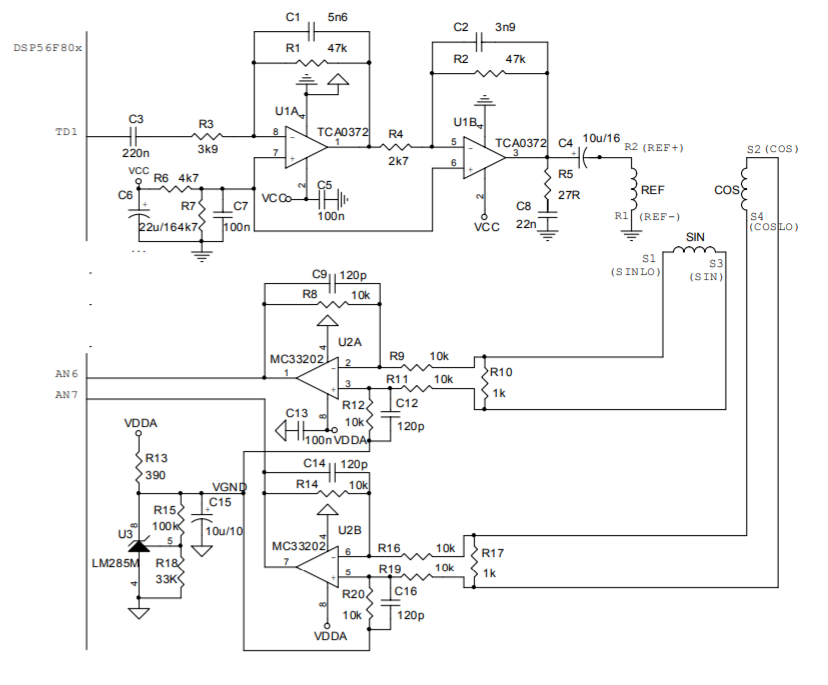
\includegraphics[width=\textwidth]{graphics/Schema_Resolver.png}
	\caption{Schema Resolver der Firma NXP.\cite{mienkina_56f80x_nodate}}
	\label{fig:Schaltung_Resolver_NXP}
\end{figure}

\paragraph{Opamp1:}\mbox{}\\

Das Dreiecksignal soll innert einer halben Periodendauer um drei Volt steigen. Das heisst, es ergibt sich gemäss Formel \ref{equ:Anstiegsrate_U1A} eine Slew-Rate von 0.048V/\textmu s.
Der auf 5.6nF dimensionierte Kondensator wird so gemässs Formel \ref{equ:Strom_C2} einen maximalen Strom von 269 \textmu A leiten. \cite{user_gast_berechnung_2009}

\begin{equation}
Slew-Rate_1 (SR_1) = \frac{\Delta_{U_1}}{T/2} = \frac{3V}{62.5 \mu s} = 0.048\frac{V}{\mu s}
\label{equ:Anstiegsrate_U1A}
\end{equation}

\begin{equation}
I_{C_2} = C_2 \cdot Slew-Rate_1 = 5.6 \cdot 10^{-9} \cdot 0.048\frac{V}{10^{-6}s} = 269\mu A
\label{equ:Strom_C2}
\end{equation}

So kann gemäss Formel \ref{equ:Dimensionierung_R1} der Widerstand R3 dimensioniert werden. Dessen Wert beträgt ungefähr 9300\textOmega. \cite{user_gast_berechnung_2009}

\begin{equation}
R3 = \frac{\pm  2.5V}{I_{C1}} = \frac{\pm 2.5V}{269 \mu A} = 9.3k\textOmega
\label{equ:Dimensionierung_R1}
\end{equation}

Mit dem Widerstand R1 und der Kapazität C2 kann die obere Grenzfrequenz bestimmt werden. Diese Grössen wurde aus dem Datenblatt des NXP-Interfaces übernommen und ergaben zusammen gmäss Formel \ref{equ:Grenzfrequenz1} eine Frequenz von:

\begin{equation}
\omega_{g1} = \frac{1}{R2 \cdot C2} = 3799 rad^{-1}
\label{equ:Grenzfrequenz1}
\end{equation}

\paragraph{Opamp2:}\mbox{}\\

Der zweite Opamp integriert das Dreiecksignal zu einem sinusförmigen Signal. Da das Ausgangssignal für die Spule 5V betragen soll und diese Änderung auch in 62.5\textmu s geschehen soll, benötigen wir eine Slew-Rate von 0.08V/\textmu s, wie mit Formel \ref{equ:Anstiegsrate_U1B} berechnet. Der daraus maximal resultierende Strom ergibt mit der in Formel \ref{equ:Strom_C3} 624 \textmu A.

\begin{equation}
Anstiegsrate_2 (SR_2) = \frac{\Delta_{U_2}}{T/2} = \frac{5V}{62.5 \mu s} = 0.08\frac{V}{\mu s}
\label{equ:Anstiegsrate_U1B}
\end{equation}

In Formel \ref{equ:Strom_C3} ist der Faktor 2 zu beachten. Dieser wird verwendet, da der Eingangsstrom dreieckförmig ist. Grundlage ist, dass die Spannung über dem Kondensator das Integral des Stromes über die Zeit ist. So ergibt sich beim Integrieren eine Fläche mit einer Spannungsamplitude von 3V mal eine Zeit von 62.6\textmu s geteilt durch 2.

\begin{equation}
I_{C_3} = C_3 \cdot Slew-Rate_2  \cdot 2= 3.9 \cdot 10^{-9} \cdot 0.080\frac{V}{10^{-6}s}  \cdot 2 = 624 \mu A
\label{equ:Strom_C3}
\end{equation}

Aus dem Maximalstrom kann der Widerstand R4 dimensioniert werden. Er beträgt ziemlich genau 2400\textOmega.

\begin{equation}
R4 = \frac{\pm 1.5V}{I_{C3}} = \frac{\pm 1.5V}{624 \mu A} = 2.4k\textOmega
\label{equ:Dimensionierung_R4}
\end{equation}

Mit dem Widerstand R2 und der Kapazität C3 kann die obere Grenzfrequenz bestimmt werden. Diese Grössen wurden aus dem Datenblatt des NXP-Interfaces übernommen und ergaben zusammen gmäss Formel \ref{equ:Grenzfrequenz2} eine Frequenz von:

\begin{equation}
\omega_{g2} = \frac{1}{R2 \cdot C3} = 5456 rad^{-1}
\label{equ:Grenzfrequenz2}
\end{equation}

\paragraph{Opamp3}\mbox{}\\

Das zurückkommende Signal muss auch gefiltert und verstärkt werden, sodass es in einem Spannungsbereich zwischen 1V und 4V liegt. Das Übersetzungsverhältnis des Resolvers beträgt 2:1, weswegen eine Spannung von \textpm \textDelta U von $\pm$ 1.25V erwartet wird. Der Differenzverstärker hat somit den Verstärkungsfaktor gemäss Formel \ref{equ:Simulation_Verstaerkungsfaktor1} von 1.2.

\begin{equation}
V = 3V/2.5V V = \frac{U_A}{U_E} = \frac{3V}{2.5V} = 1.2
\label{equ:Simulation_Verstaerkungsfaktor1}
\end{equation}

Daraus kann der Widerstand R12 berechnet werden. Dieser Beträgt gemäss Formel \ref{equ:Simulation_R12} 12k\textOmega.

\begin{equation}
R12 = V \cdot R9 = 1.2 \cdot 10k\Omega = 12k\Omega
\label{equ:Simulation_R12}
\end{equation}

Die Kondensatorgrösse wurde aus dem Datenblatt von NXP übernommen. Damit wird jedoch die Grenzfrequenz festgelegt. Diese ergibt mit R12 und C6 gemäss Formel \ref{equ:Grenzfrequenz3} 644444 rad$^{-1}$

\begin{equation}
\omega_{g2} = \frac{1}{R12 \cdot C6} = 644.44 krad^{-1}
\label{equ:Grenzfrequenz3}
\end{equation}

\subsubsection{Simulation}

Die berechneten Werte wurden in der Simulation eingesetzt. Da die Opamps und der Kondensator C1 die Schaltung beeinflussen, wurden kleine Anpassungen an den Werten von R3 und R4 gemacht, um die gewünschten Effekte zu erlangen. Die Simulationsergebnisse werden im Folgenden aufgelistet:
\begin{itemize}
\item C1 = 220nF
\item C2 = 5.6nF
\item C3 = 3.9nF
\item R1 = 9k\textOmega
\item R2 = 47k\textOmega
\item R3 = 47k\textOmega
\item R4 = 2.5k\textOmega
\end{itemize}

%Die Rück-Berechnung zur Amplitude des Ausgangssignals erhalten wir über:
%
%\begin{equation}
%I_{C1}=\frac{\pm2.5V}{R1} = \frac{\pm2.5V}{10k\Omega} = \pm 250 \mu A => \Delta_{I_{C1}} = 500\mu A
%\end{equation}
%
%mit:
%
%\begin{equation}
%Anstiegsrate = \frac{I_{C1}}{C1} = 
%\end{equation}
%
%ergibt:
%
%\begin{equation}
%\Delta U = \frac{Anstiegsrate \cdot T}{2}
%\end{equation}


%Die Spule am Referenzsignal hat einen ohmischen Widerstand von 55\textOmega, was gemäss Formel \ref{equ:Spulenstrom}zu einem Spitzenstrom von 90mA ergibt.

%\begin{equation}
%\^{I}_{Spule} = \frac{\^{U}_{Spule}}{R_{Spule}} = \frac{5V}{55\textOmega} = 0.09A = 90mA
%\label{equ:Spulenstrom}
%\end{equation}

Abbildung \ref{fig:Simulation_Referenzsignal} zeigt die Opamp-Schaltung für das Referenzsignal. Darin enthalten sind die beiden Verstärkerschaltungen in Serie geschaltet. Beide haben einen Offset von 2.5V. Der Kondensator C1 bildet einen Hochpass, woduch sich die Spannungen in der gesamten Schaltung ein wenig anheben und es eine Weile dauert, bis die Schaltung eingeschwungen ist.Die passiven Elemente R5 und C4 verhindern ein ungewolltes Schwingen des Ausgangs, wenn induktive Lasten angetrieben werden.
Abbildung \ref{fig:Simulation_Referenzsignal2} zeigt die Differenzverstärkerschaltung auf Empfängerseite.

\begin{figure}[h!]
\centering
\subcaptionbox{Schema Simulation Referenzsignal.\label{fig:Simulation_Referenzsignal}}{	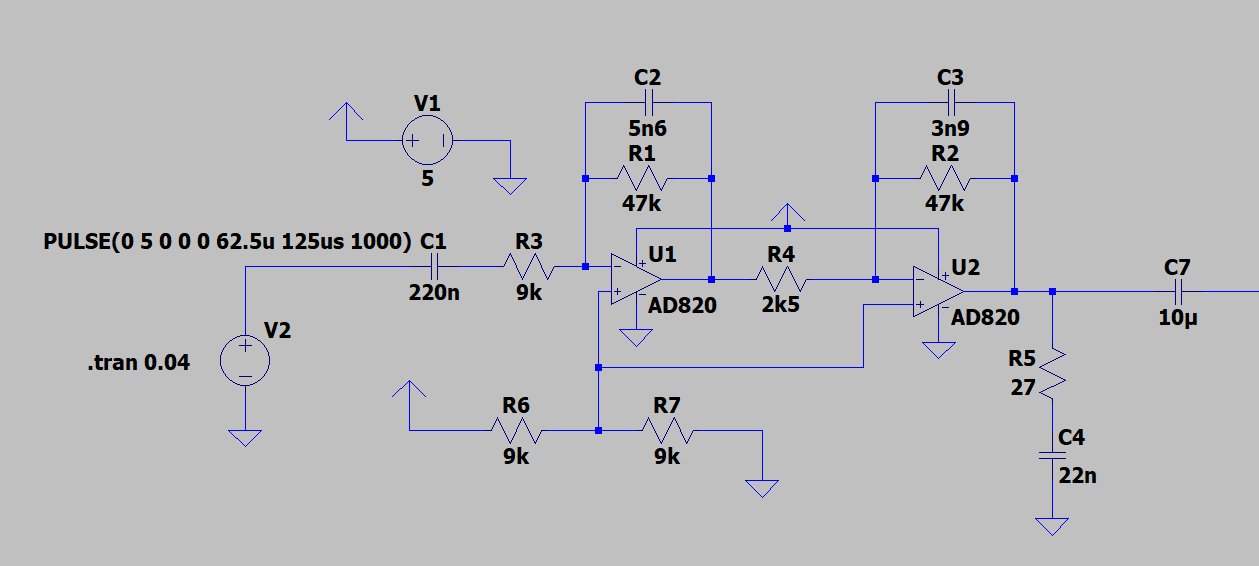
\includegraphics[height=4.5cm]{graphics/Simulation_Schema_Referenzsignal.png}}
\hfill
\subcaptionbox{Schema Simulation Referenzsignal.\label{fig:Simulation_Referenzsignal2}}{	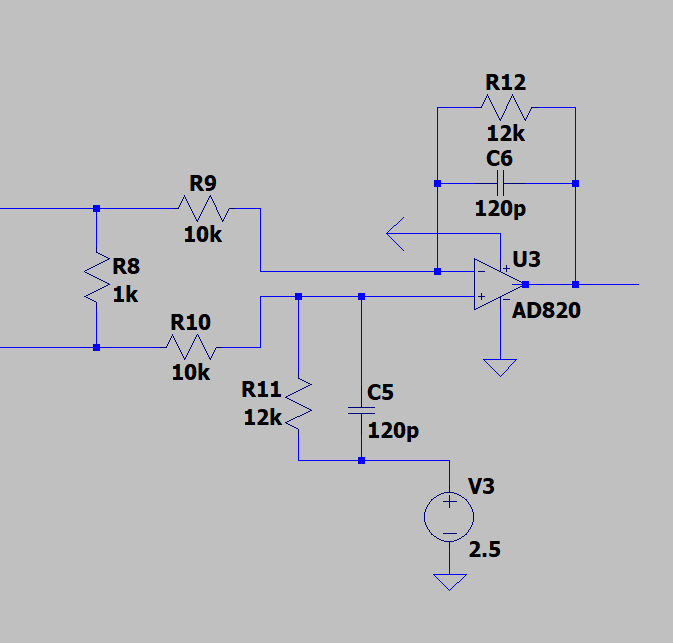
\includegraphics[height=4.5cm]{graphics/Simulation_Schema_Referenzsignal2.png}}
\hfill
\caption{Schema Simulation Referenzsignal Resolver.}
\label{fig:Simulation_Referenzsignal0}
\end{figure}

\newpage
In Abbildung \ref{fig:Simulation_Einschwingvorgang} ist der Einschwingvorgang zu erkennen. Das gesamte System ist nach etwa 20 ms eingeschwungen. Das blaue Signal ist die Spannung zwischen dm Kondensator C1 und R1, das grüne Signal ist das Dreiecksignal am Ausgang des ersten Opamps und das rote Signal ist das Sinus-Signal am Ausgang des zweiten Opamps.

\begin{figure}[h!]
	\centering
	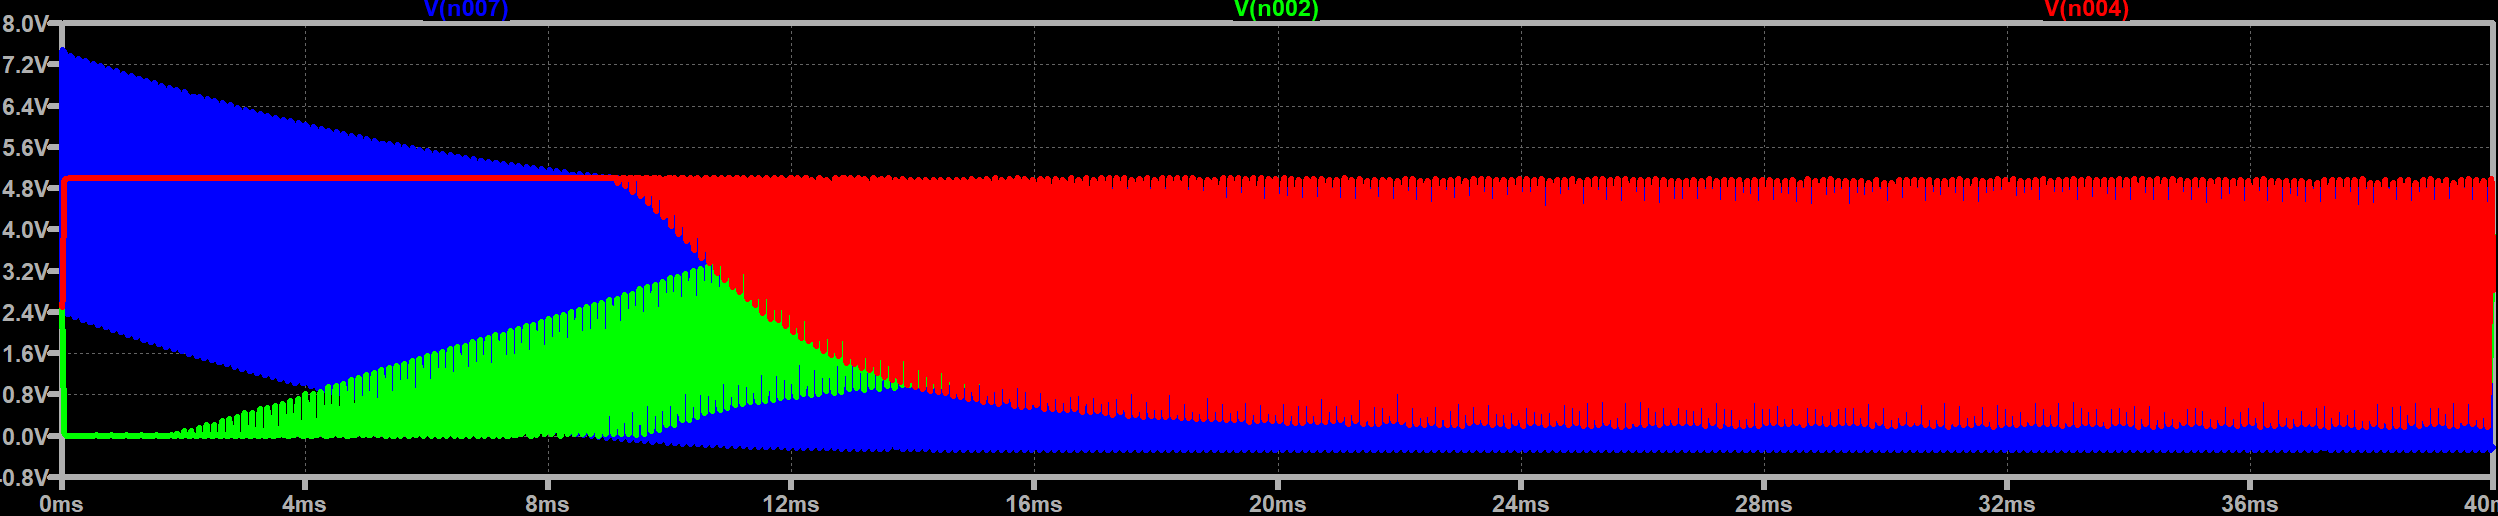
\includegraphics[width=\textwidth]{graphics/Einschwingvorgang.png}
	\caption{Einschwingvorgang}
	\label{fig:Simulation_Einschwingvorgang}
\end{figure}

%Beide Operationsverstärker werden mit Single-Supply versorgt, weshalb ein virtueller Ground erstellt wird mit den Widerständen \textbf{R704 und R706}. So Pendelt das Signal um die 2.5V Referenzspannung. Erwünscht ist ein Ausgangssignal zwischen 0 und 5 V, das heisst, dass eine Amplitude von 2.5 angestrebt wird.

%Die Schaltung wurde in LTSpice aufgebaut, um das Verhalten zu untersuchen. Folgende Resultate wurden erzielt:

%Wird nun ein Rechtecksignal eingespiesen, wird dieses Integriert. Abbildung \ref{fig:Simulation_Rechteck_Dreieck} zeigt das Rechtecksignal und das daraus resultierende Dreiecksignal.

In den Abbildungen \ref{fig:Simulation_Rechteck_Spannung} und \ref{fig:Simulation_Rechteck_Strom} ist die Spannung und der Strom am und durch den Punkt zwischen C1 und R3 zu sehen. Der Strom durch C1 und R1 ist folglich der selbe. Die Spannung an diesem Punkt ist das Eingangssignal für die Integratorschaltung am Opamp1.
\begin{figure}[h!]
	\centering
	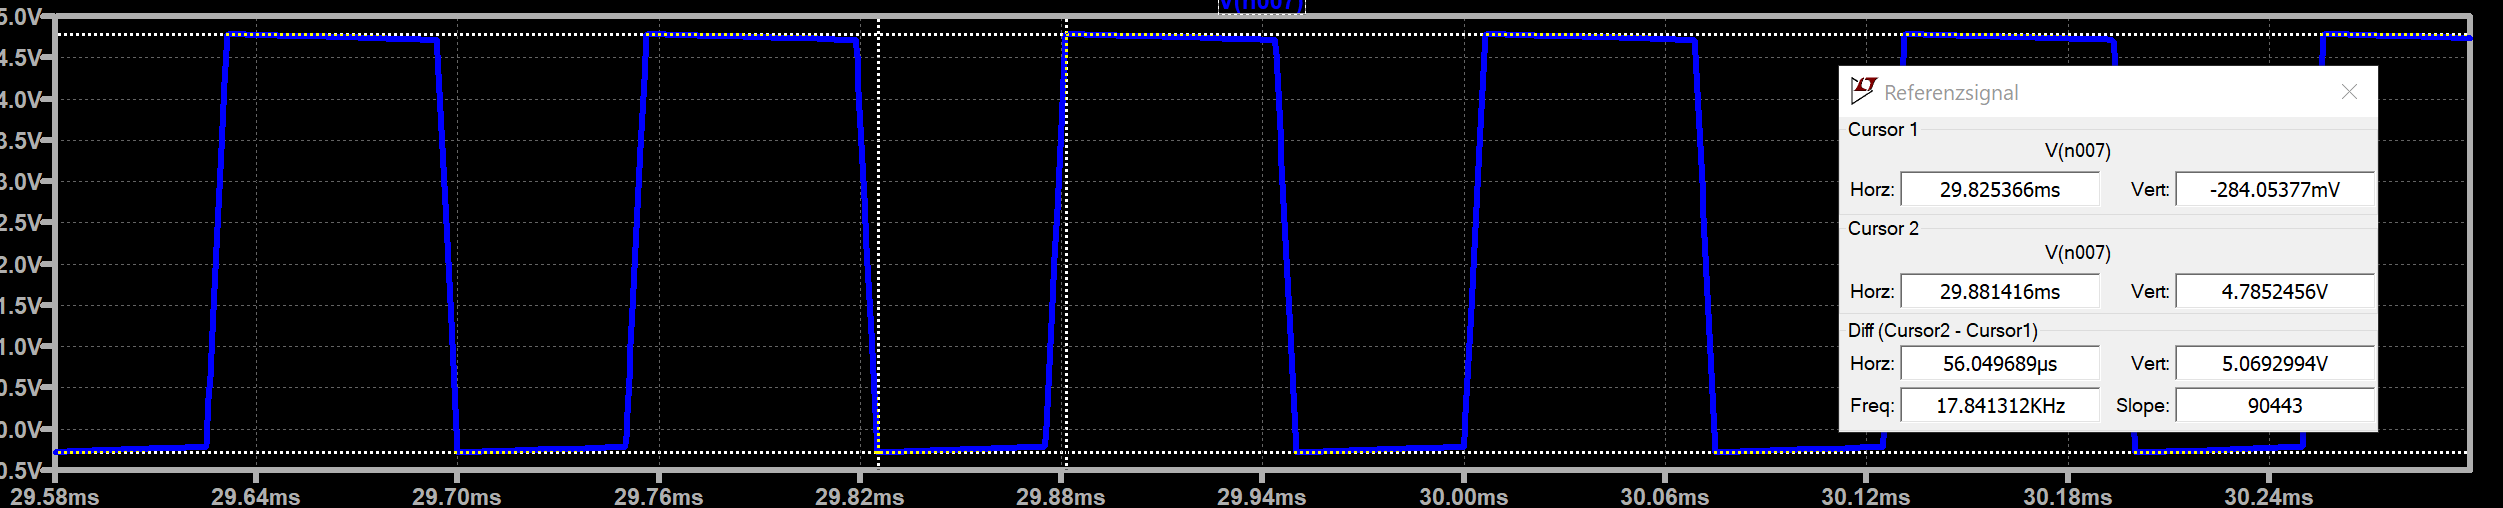
\includegraphics[width=\textwidth]{graphics/Spannung_Ue_1.png}
	\caption{Eingangs PWM-Signal zwischen C1 und R1. Zu erkennen: Durch den Strom durch R3 fällt eine Spannung über dem Widerstand ab. Der Spannungsabfall lässt sich im Rest der Schaltung nicht gross bemerken.}
	\label{fig:Simulation_Rechteck_Spannung}
\end{figure}

%
%Abbildung \ref{fig:Simulation_Dreieck_Sinus} zeigt das Sinussignal (grün), welches aus dem Dreieck generiert wurde. Sie zeigt ebenfalls das Signal, wie es aus dem Resolver zurückgegeben würde.

\begin{figure}[h!]
	\centering
	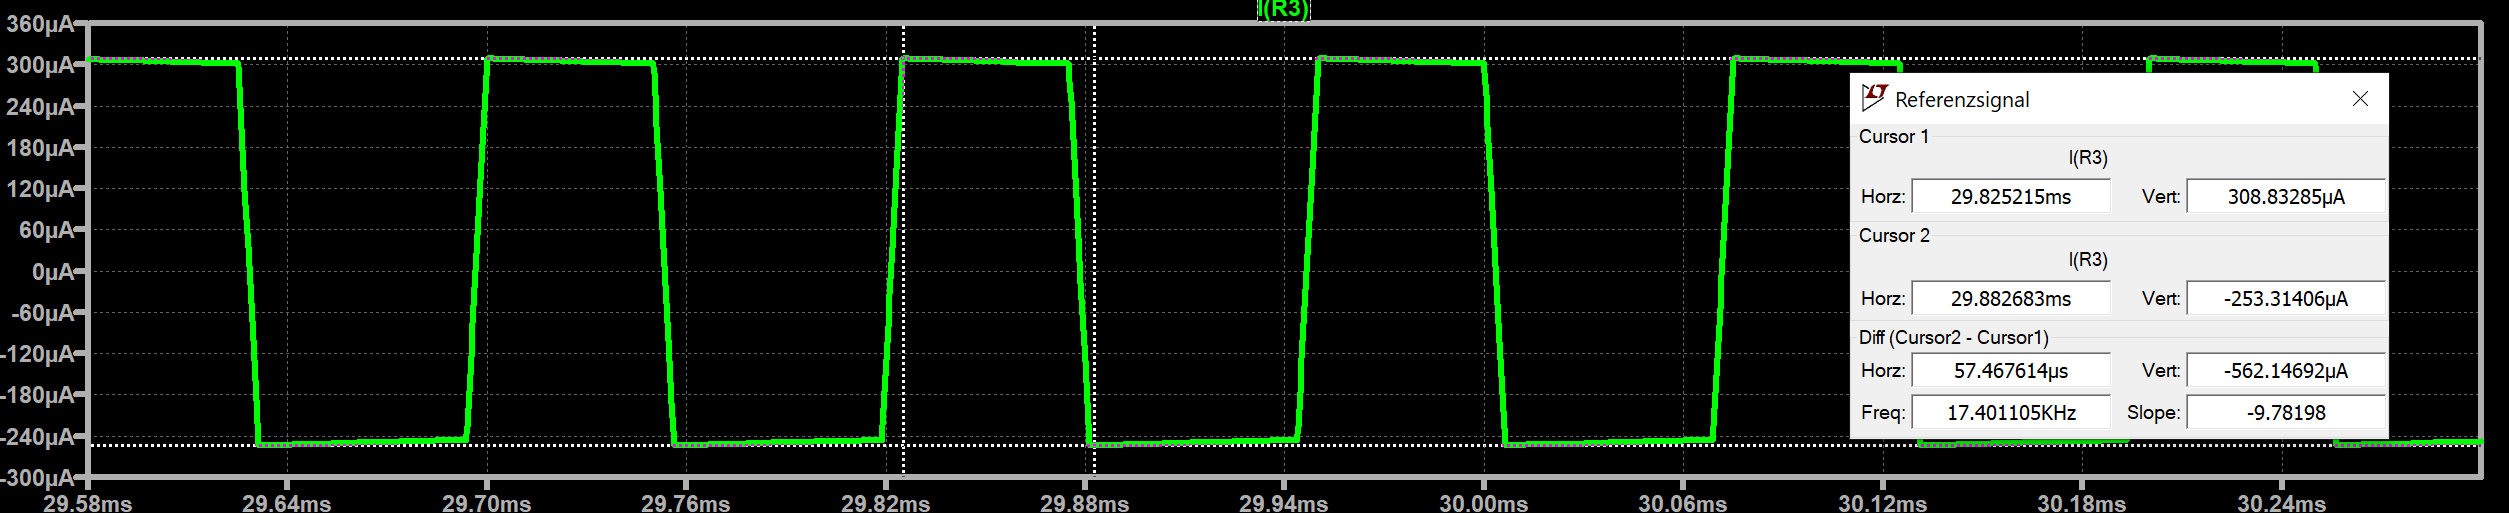
\includegraphics[width=\textwidth]{graphics/Strom_Ic1.png}
	\caption{Eingangs-Strom durch R3. Zu erkennen: Der halbe Strom I$_{P-P}$ beträgt 281\textmu A und ist somit leicht höher als in Formel \ref{equ:Strom_C2} berechnet.
	%Dies hat damit zu tun, dass der Widerstand durch Anpassungen an dessem Wert kleiner gewählt wurde. Der Strom durch den Widerstand R1 ist so klein, dass er vernachlässigt werden kann.
	}
	\label{fig:Simulation_Rechteck_Strom}
\end{figure}

\newpage

In den Abbildungen \ref{fig:Simulation_Dreieck_Spannung} und \ref{fig:Simulation_Dreieck_Strom} ist die Spannung am Ausgang vom Opamp1 und der Strom durch R4 abgebildet. Die Ausgangsspannung vom Opamp1 ist das Eingangssignal des Opamp2. 
%Die Übertragungsfunktion wurde anhand eines Bode-Plots in Abbildung \ref{fig::Simulation_Bode_1} dargestellt.

\begin{figure}[h!]
	\centering
	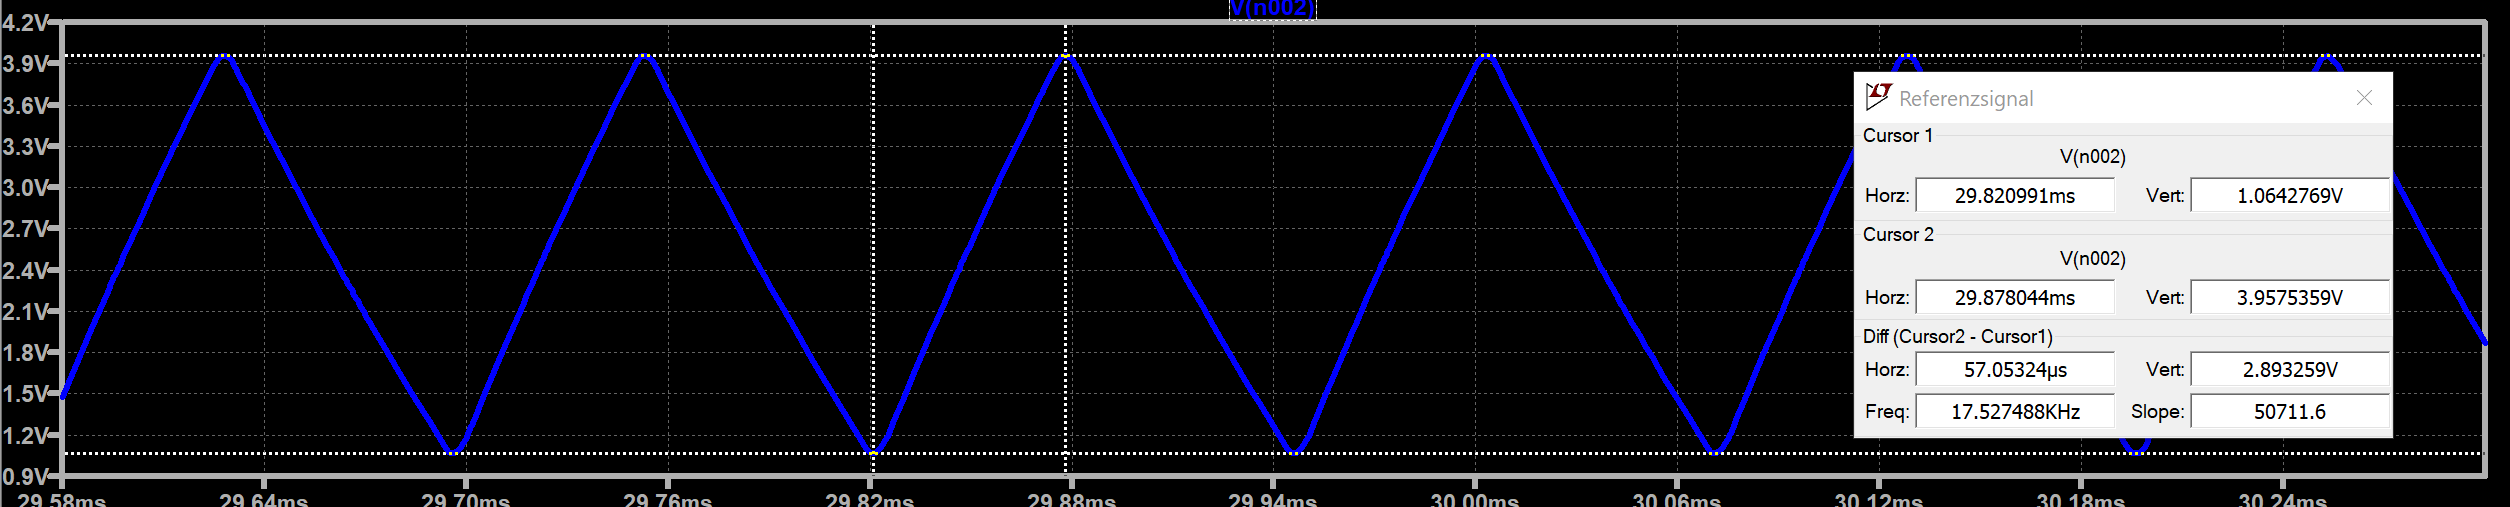
\includegraphics[width=\textwidth]{graphics/Spannung_Ua_1.png}
	\caption{Spannung am Ausgang des Opamp1. Zu erkennen: Die Peak-to-Peak-Amplitude beträgt grössenordnung 2.9V. Dies lässt sich auf die verzögerten Flanken des Opamps zurückführen, da mit einem idealen Opamp gerechnet wurde.}
	\label{fig:Simulation_Dreieck_Spannung}
\end{figure}

\begin{figure}[h!]
	\centering
	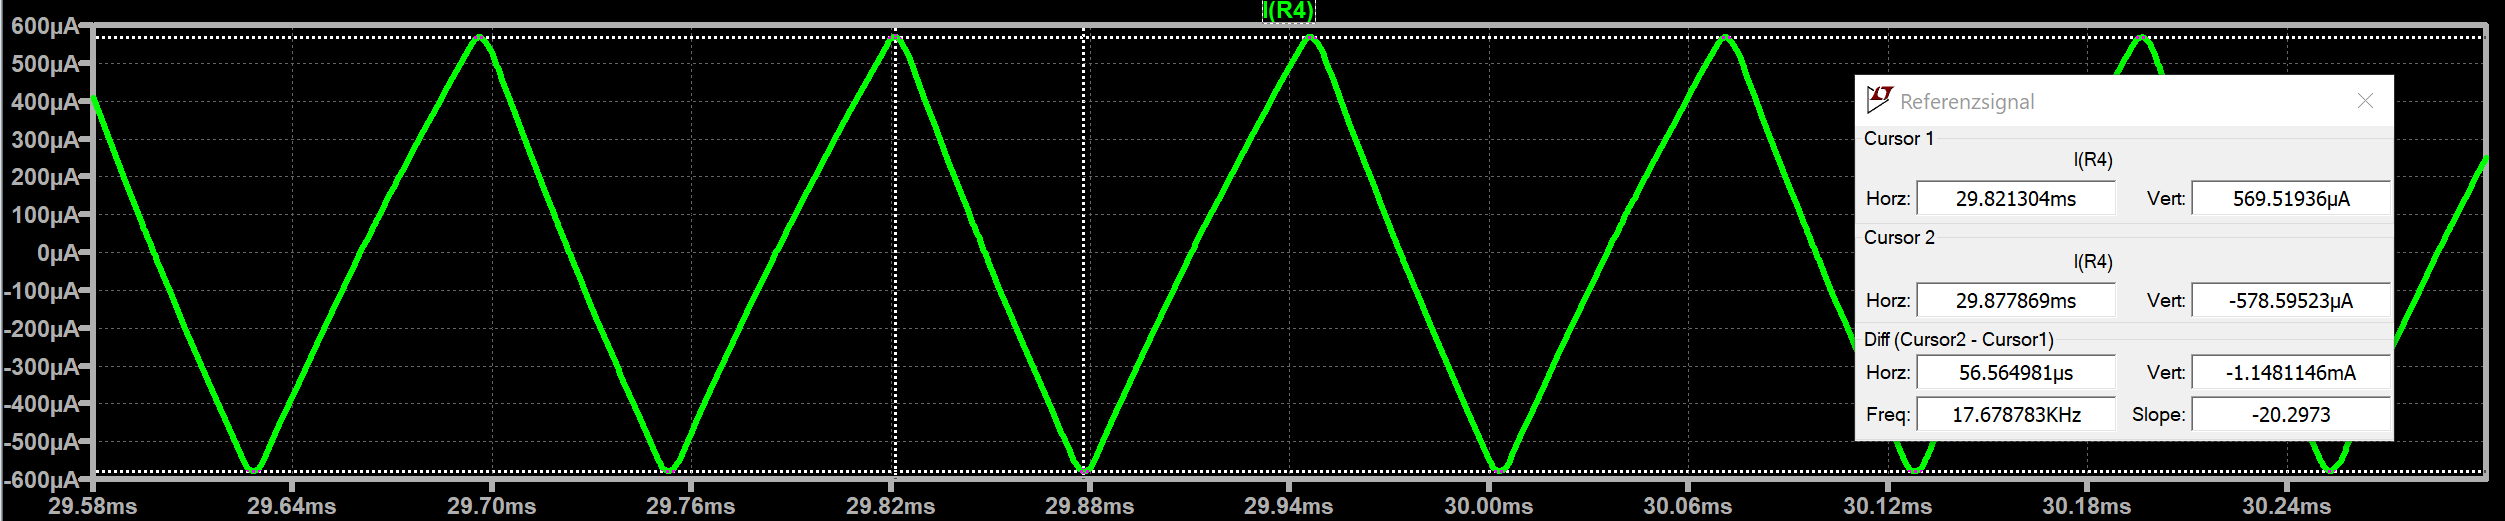
\includegraphics[width=\textwidth]{graphics/Strom_Ir_2.png}
	\caption{Eingangs-Strom durch R4. Zu erkennen: Der halbe Strom I$_{P-P}$ beträgt 574\textmu A und ist somit leicht tiefer als in Formel \ref{equ:Strom_C2} berechnet.
	%Dies hat damit zu tun, dass der Widerstand durch Anpassungen an dessem Wert grösser gewählt wurde. Der Strom durch den Widerstand R3 ist so klein, dass er vernachlässigt werden kann.
	}
	\label{fig:Simulation_Dreieck_Strom}
\end{figure}

%\begin{figure}[h!]
%	\centering
%	\includegraphics[width=0.5\textwidth]{graphics/Op1.png}
%	\caption{Bodeplot Übertragungsfunktion Opamp1.}
%	\label{fig:Simulation_Bode_1}
%\end{figure}

In den Abbildungen \ref{fig:Simulation_Sinus_Spannung} und \ref{fig:Simulation_Sinus_Strom} ist die Spannung am Ausgang vom Opamp1 und der Strom durch R4 abgebildet. Die Spannung am Ausgang vom Opamp1 ist das Eingangssignal des Opamp2.  
%Die Übertragungsfunktion vom Opamp2 wurde anhand eines Bode-Plots in Abbildung \ref{fig:Simulation_Bode_2} dargestellt. Die Abbildung \ref{fig:Simulation_Bode_3} zeigt die Übertragungsfunktion der beiden Operationsverstärkerschaltungen in Serie.

\begin{figure}[h!]
	\centering
	\includegraphics[width=\textwidth]{graphics/Spannung_Ua_3.png}
	\caption{Spannung am Ausgang des Opamp2. Zu erkennen: Die Peak-to-Peak-Amplitude beträgt grössenordnung 4.8V. Dies lässt sich auf die verzögerten Flanken des Opamps (idealer Opamp) und das ohnehin schon weniger starke Dreiecksignal zurückführen.}
	\label{fig:Simulation_Sinus_Spannung}
\end{figure}
\begin{figure}[h!]
	\centering
	\includegraphics[width=\textwidth]{graphics/Strom_Ir_3.png}
	\caption{Strom durch R2.}
	\label{fig:Simulation_Sinus_Strom}
\end{figure}
%\begin{figure}[h!]
%	\centering
%	\includegraphics[width=0.5\textwidth]{graphics/Op2.png}
%	\caption{Bodeplot Übertragungsfunktion Opamp2.}
%	\label{fig:Simulation_Bode_2}
%\end{figure}

%\begin{figure}[h!]
%	\centering
%	\includegraphics[width=0.5\textwidth]{graphics/Op1_Op2.png}
%	\caption{Bodeplot Übertragungsfunktion Opamp1 $\cdot$ Opamp2.}
%	\label{fig:Simulation_Bode_3}
%\end{figure}

In den Abbildungen \ref{fig:Simulation_Op3_1} und \ref{fig:Simulation_Op3_2} ist die Spannung am Ausgang vom Opamp3 und der Strom durch R9 abgebildet. Die Spannung am Ausgang vom Opamp3 ist das Eingangssignal des TMC4671. Die Ausgangsspannung für den Controller ist in Abbildung \ref{fig:Simulation_Op3_3} dargestellt.

\begin{figure}[h!]
	\centering
	\includegraphics[width=\textwidth]{graphics/Spannung_Ue_2.png}
	\caption{Eingangsspannung für Verstärkerschaltung Mikrocontrollersignal.}
	\label{fig:Simulation_Op3_1}
\end{figure}

\begin{figure}[h!]
	\centering
	\includegraphics[width=\textwidth]{graphics/Strom_Ir_4.png}
	\caption{Strom durch Widerstand R9.}
	\label{fig:Simulation_Op3_2}
\end{figure}

\begin{figure}[h!]
	\centering
	\includegraphics[width=\textwidth]{graphics/Spannung_Ua_4.png}
	\caption{Ausgangsspannung für TMC4671. Zu erkennen: Das Signal liegt zwischen 1V und 4V, wie es der Controller braucht.}
	\label{fig:Simulation_Op3_3}
\end{figure}

%\begin{figure}[h!]
%	\centering
%	\includegraphics[width=0.5\textwidth]{graphics/Op3.png}
%	\caption{Bodeplot Übertragungsfunktion Opamp3.}
%	\label{fig:Simulation_Bode_4}
%\end{figure}

\newpage
\subsection{Pumpenansteuerung}
\label{subsec:Detailkonzept_Pumpenansteuerung}

Die 12 Pumpen werden direkt über den Mikrokontroller via Digitalausgänge angesteuert. Da jedoch der Mikrokontroller nicht genügend Strom liefern kann, wird ein Logik-MOSFET eingesetzt. Bei dem MOSFET handelt es sich um einen IRLR8726 von Infineon. Mit diesem wurde schon in früheren Projekten gearbeitet, bei welchen sich dieser als zuverlässig herausstellte. Dieser MOSFET zeichnet sich durch einen geringen R$_{DSon}$ von 5.8m$\Omega$, eine kleine Gatekapazität von 15nC, einer V$_{DS}$ Breakdownvoltage von 30V und einer hohen Strombelastbarkeit von maximal 86A aus. Die Ansteuerung ist relativ simpel aufgebaut und kann in Abbildung \ref{fig:Pumpenansteuerung} begutachtet werden. 

\begin{figure}[h!]
\centering
\includegraphics[width=0.6\textwidth]{graphics/Pumpenansteuerung.png}
\caption{Schema der Pumpenansteuerung}
\label{fig:Pumpenansteuerung}
\end{figure} 

Um den Gate-Eingang zu schonen, wird ein 10$\Omega$ Widerstand vogeschaltet. Parallel zur Pumpe ist eine Freilaufdiode verbaut, welche den Drain-Eingang der MOSFETS beim Ausschalten der Pumpe vor Spannungsspitzen schützt. 

\subsection{Durchflussmessgeräte}
\label{subsec:Detailkonzept_Durchflussmessgeräte}

Um die Durchflussmessgeräte ansteuern zu können, wird keine zusätzliche Elektronik benötigt. Es wird lediglich eine 5V Speisung sowie ein Analog- oder Digitaleingang eines Mikrocontrollers benötigt. Dabei wird jedoch ein Digitaleingang bevorzugt, da keine unterschiedlichen Spannungen eingelesen werden müssen, sondern lediglich High- und Lowpegel. Das Durchflussmessgerät sendet somit bei laufender Umdrehungszahl ein gepulstes Signal, welches mit steigendem Durchfluss die Frequenz erhöht. Dies geschieht bei gleichbleibendem Duty-Cycle von 50\%.

\newpage
\subsection{Display}\label{subsubsec:Detailkonzept_Display}

Beim Display handelt es sich um das in Kapitel \ref{subsubsec:Grobkonzept_Display} evaluierte 7" Display von Nextion. Genauer gesagt um de Typ NX8048T070. Dieses wird über eine UART-Schnittstelle angesteuert und wird mit 5V gespiesen. Das verwendete Display ist in Abbildung \ref{fig:Nextion_Display} zu sehen.

\begin{figure}[h!]
\centering
\includegraphics[width=0.7\textwidth]{graphics/Nextion_Display.jpg}
\caption{Ansichtsbild des verwendeten Display's. \cite{made-in-china_nextion_nodate}}
\label{fig:Nextion_Display}

\end{figure}

Um mit diesem Displaytyp arbeiten zu können, ist es wichtig, dass man sich einen Überblick über die Eigenschaften verschafft. Die wichtigsten Eigenschaften des Display's können in Tablle \ref{tab:Eigenschaften_Nextion_Display} eingesehen werden.

\begin{table}[h!]
\centering
\begin{tabularx}{0.6\textwidth}{|X|p{2.8cm}|}
\hline
\textbf{Speisespannung:} & 5V
\\
\hline
\textbf{Arbeitsstrom:} & 510mA
\\
\hline
\textbf{Sleep-Mode Strom:} & 15mA
\\
\hline
\textbf{Arbeitstemperatur:} & -20\textdegree bis 70\textdegree
\\
\hline
\textbf{Flash Speicher:} & 16MB
\\
\hline
\textbf{RAM Speicher:} & 3584BYTE
\\
\hline
\textbf{Farben:} & 65536 Farben
\\
\hline
\textbf{Auflösung:} & 800*480
\\
\hline
\textbf{Touch Typ:} & resistiv
\\
\hline
\textbf{Hintergrundbeleuchtung:} & LED
\\
\hline
\end{tabularx}
\caption{Eigenschaften des Nextion Display's \cite{patrick_nx8048t070_nodate}.}
\label{tab:Eigenschaften_Nextion_Display}
\end{table}

Die zwei grössten Vorteile dieses Displaytyps sind die Entwicklungsumgebung, sowie die grosse Community. Nextion bietet von sich aus einen GUI-Editor (Graphical User Interface Editor) an, welcher gratis zur Verfügung gestellt wird. Mit Hilfe dieses Tools können spielend leicht grafische Oberflächen geschaffen werden mit verschiedensten Komponenten wie Tasten, Textfelder, Bilder, Slider und viele mehr. Die Oberfläche des Editors kann in Abbildung \ref{fig:Nextion_Editor} begutachtet werden.

\begin{figure}[h!]
\centering
\includegraphics[width=\textwidth]{graphics/Nextion_Editor.png}
\caption{Entwicklungsumgebung von Nextion (Nextion Editor).}
\label{fig:Nextion_Editor}
\end{figure}

Die Software ist so einfach wie möglich gehalten. Im roten Feld 1 können Komponenten wie Slider, Textfelder, Tasten ect. per Klick in die erstellte Displayoberfläche im orangen Feld 2, im Ansichtsfenster eingefügt werden. In diesem Feld ist zu sehen, was schlussendlich auf dem Display ersichtlich ist. Es können natürlich mehrere Displayseiten erstellt werden. Diese können im gelben Feld 3 hinzugefügt, gelöscht oder umbenannt werden. Per Klick auf die gewünschte Seite wird diese im Ansichtsfenster 2 angezeigt und kann dann bearbeitet werden. Im grünen Feld 4 befinden sich die Eigenschaften der Elemente der erstellten Displayseite. Wird ein Element auf der Displayseite angeklickt, so erscheinen dort dessen Eigenschaften. Diese können dann beliebig angepasst werden. Dazu gehören zum Beispiel die Elementgrösse oder die Platzierungsposition. Im blauen Feld 5 kann den einzelnen Elementen ein Reaktionsbefehl gegeben werden. Dabei kann ausgewählt werden, ob das Element auf Drücken, Loslassen oder beides Reagieren soll. Ausserdem können dort Befehle eingegeben werden. Also zum Beispiel bei einem Taster: ``page 2``. Dies bedeutet so viel wie: ``Falls das Element gedrückt wird, dann zeige Displayseite 2 an``. Natürlich können so auch Befehle über die UART-Schnittstelle weiter gegeben und empfangen werden. Das violette Feld 6 bietet eine Outputübersicht an, welche zu Simulationszwecken verwendet wird. Im letzten grauen Feld 7 können Vorlagen abgespeichert werden. Dazu gehören Bilder, Textstyle Vorlagen, Audio- und Videodateien.

\subsection{User Interface}\label{subsubsec:Detailkonzept_UserInterface}

Um die Cocktailmaschine schlussendlich sauber bedienen zu können, wird das in Kapitel \ref{subsec:Hardware_Display} beschriebene Display als Benutzerschnittstelle fungieren. Weitere Schnittstellen werden erstmal nicht verwendet. Damit der Benutzer jedoch die Maschine möglichst intuitiv und einfach bedienen kann, muss zuerst eine geeignete Menustruktur erstellt werden. Im Projekt 5 wird noch nicht die gesamte Struktur auf dem Display programmiert. Trotzdem wird die gesamte Struktur erarbeitet, damit klar ist, welche Schnittstellen benötigt werden. Somit kann ein Testprogramm erstellt werden, welches alle später benötigten Schnittstellen und Funktionen testet. Das komplette Programm wird in Projekt 6 erstellt. Die erarbeitete Menustruktur sieht wie folgt aus.

\subsubsection{Startanzeige}\label{subsubsec:Display_Startanzeige}

Auf der Startanzeige \ref{fig:Display_Startanzeige} kann mit den Pfeiltasten ein gewünschter Cocktail ausgewählt werden. Dabei wird immer ein Bild des Cocktails mit dem dazugehörigen Namen angezeigt. Wird auf den Button «Zutaten» gedrückt erscheint die Zutatenanzeige \ref{fig:Display_Zutatenanzeige}. Wird auf den Button «Menu» gedrückt so gelangt man in die Menuanzeige \ref{fig:Display_Menuanzeige}. Wird auf den Cocktail gedrückt, so gelangt man in die Zubereitungsabfrage \ref{fig:Display_Zubereitungsabfrage}. Mit dem Button «Ohne Alkohol» oder «Mit Alkohol» kann zwischen alkoholischen und nicht alkoholischen Cocktails ausgewählt werden. Wird der Button «Liste» betätigt, so wird die Listenanzeige \ref{fig:Display_Listenanzeige} der alkoholischen oder nicht alkoholischen Cocktails angezeigt.

\begin{figure}[h!]
\centering
\includegraphics[width=0.7\textwidth]{graphics/Display_Startanzeige.png}
\caption{Ansichtsbild Startanzeige}
\label{fig:Display_Startanzeige}
\end{figure}

\subsubsection{Zutatenanzeige}\label{subsubsec:Display_Zutatenanzeige}

In der Zutatenanzeige \ref{fig:Display_Zutatenanzeige} wird dem Kunden eine Übersicht über die beinhaltenden Zutaten des ausgewählten Cocktails gegeben. Um aus der Zutatenanzeige zu gelangen, kann mit «OK» bestätigt werden.

\begin{figure}[h!]
\centering
\includegraphics[width=0.7\textwidth]{graphics/Display_Zutatenanzeige.png}
\caption{Ansichtsbild Zutatenanzeige}
\label{fig:Display_Zutatenanzeige}
\end{figure}

\subsubsection{Listenanzeige}\label{subsubsec:Display_Listenanzeige}

In der Listenanzeige \ref{fig:Display_Listenanzeige} wird dem Kunden eine Liste der verfügbaren Cocktails aufgezeigt, wobei dieser mit den Pfeiltasten durchblättern und den gewünschten Cocktail auswählen kann. Wird auf einen Cocktail gedrückt, so gelangt man wieder in die Startanzeige \ref{fig:Display_Startanzeige} mit dem ausgewählten Cocktail.

\begin{figure}[h!]
\centering
\includegraphics[width=0.7\textwidth]{graphics/Display_Listenanzeige.png}
\caption{Ansichtsbild Listenanzeige}
\label{fig:Display_Listenanzeige}
\end{figure}

\subsubsection{Zubereitungsabfrage}\label{subsubsec:Display_Zubereitungsabfrage}

In der Zubereitungsabfrage \ref{fig:Display_Zubereitungsabfrage} wird der Kunde gefragt, ob er einen 3dl oder 5dl Cocktail zubereiten will. Wird «Ja 3dl» betätigt, so wird ein 3dl Getränk zubereitet. Wird «Ja 5dl» betätigt, so wird ein 5dl Getränk zubereitet und man gelangt auf den Zubereitungsbildschirm \ref{fig:Display_Zubereitungsbildschirm}. Mit «Abbrechen» gelangt man zurück zur Startanzeige \ref{fig:Display_Startanzeige}.

\begin{figure}[h!]
\centering
\includegraphics[width=0.7\textwidth]{graphics/Display_Zubereitungsabfrage.png}
\caption{Ansichtsbild Zubereitungsabfrage}
\label{fig:Display_Zubereitungsabfrage}
\end{figure}

\subsubsection{Zubereitungsbildschirm}\label{subsubsec:Display_Zubereitungsbildschirm}

Auf dem Zubereitungsbildschirm \ref{fig:Display_Zubereitungsbildschirm} wird der Kunde darüber informiert, dass der Cocktail zubereitet wird. Gleichzeitig wird dem Kunden ein Fact zum gewählten Cocktail gezeigt, um die Wartezeit ein wenig zu versüssen. Mit dem Button «Abbrechen» kann der laufende Prozess abgebrochen werden und es erscheint die Abbruchanzeige \ref{fig:Display_Abbruchanzeige}. Ist der Cocktail fertig, so wird dem Kunden die Bereitanzeige \ref{fig:Display_Bereitanzeige} angezeigt. 

\begin{figure}[h!]
\centering
\includegraphics[width=0.7\textwidth]{graphics/Display_Zubereitungsbildschirm.png}
\caption{Ansichtsbild Zubereitungsbildschirm}
\label{fig:Display_Zubereitungsbildschirm}
\end{figure}

\subsubsection{Bereitanzeige}\label{subsubsec:Display_Bereitanzeige}

Die Bereitanzeige \ref{fig:Display_Bereitanzeige} zeigt dem Kunden, dass der Cocktail fertig ist und dieser nun entnommen werden kann. Dieser Bildschirm erscheint für 5 Sekunden. Nach dieser Zeit erscheint automatisch wieder die Startanzeige \ref{fig:Display_Startanzeige}.

\begin{figure}[h!]
\centering
\includegraphics[width=0.7\textwidth]{graphics/Display_Bereitanzeige.png}
\caption{Ansichtsbild Bereitanzeige}
\label{fig:Display_Bereitanzeige}
\end{figure}

\subsubsection{Menuanzeige}\label{subsubsec:Display_Menuanzeige}

Wird in der Menuanzeige \ref{fig:Display_Menuanzeige} «Cocktail bearbeiten» ausgewählt, so kommt man in die Bearbeitungsanzeige \ref{fig:Display_Bearbeitungsanzeige}. Wird «Maschine Reinigen» gedrückt, so gelangt man in die Reinigungsanzeige1 \ref{fig:Display_Reinigungsanzeige1}. Wird «Maschineninfo» betätigt, so gelangt man in die Infoanzeige \ref{fig:Display_Infoanzeige}. Mit «Zurück» gelangt man wieder auf den Startanzeige \ref{fig:Display_Startanzeige}.

\begin{figure}[h!]
\centering
\includegraphics[width=0.7\textwidth]{graphics/Display_Menuanzeige.png}
\caption{Ansichtsbild Menuanzeige}
\label{fig:Display_Menuanzeige}
\end{figure}

\subsubsection{Bearbeitungsanzeige}\label{subsubsec:Display_Bearbeitungsanzeige}

In der Bearbeitungsanzeige \ref{fig:Display_Bearbeitungsanzeige} kann der zu bearbeitende Cocktail ausgewählt werden. Wird einer ausgewählt, so gelangt man in die dazugehörige Cocktaileinstellungsanzeige \ref{fig:Display_Cocktaileinstellungsanzeige}. Mit den Pfeiltasten kann zwischen den verschiedenen Cocktails navigiert werden. Wird «Zurück» betätigt, so gelangt man wieder zur Menuanzeige \ref{fig:Display_Menuanzeige}. 

\begin{figure}[h!]
\centering
\includegraphics[width=0.7\textwidth]{graphics/Display_Bearbeitungsanzeige.png}
\caption{Ansichtsbild Bearbeitungsanzeige}
\label{fig:Display_Bearbeitungsanzeige}
\end{figure}

\subsubsection{Cocktaileinstellungsanzeige}\label{subsubsec:Display_Cocktaileinstellungsanzeige}

In der Cocktaileinstellungsanzeige \ref{fig:Display_Cocktaileinstellungsanzeige} kann mittels Schieberegler jede Zutat in der Menge angepasst werden. Es kann jedoch nie 100\% überschritten werden. Wird «Standarteinstellung» gedrückt, so wird der Cocktail auf die jeweilige Standarteinstellung eingestellt. Betätigt man «OK», so gelangt man wieder in die Bearbeitungsanzeige \ref{fig:Display_Bearbeitungsanzeige}.

\begin{figure}[h!]
\centering
\includegraphics[width=0.7\textwidth]{graphics/Display_Cocktaileinstellungsanzeige.png}
\caption{Ansichtsbild Cocktaileinstellungsanzeige}
\label{fig:Display_Cocktaileinstellungsanzeige}
\end{figure}

\subsubsection{Reinigungsanzeige1}\label{subsubsec:Display_Reinigungsanzeige1}

In der Reinigungsanzeige1 \ref{fig:Display_Reinigungsanzeige1} wird man Stück für Stück durch den Reinigungsmodus geführt. In der Reinigungsanzeige1 wird man aufgefordert den Reinigungsbehälter mit warmem Wasser zu befüllen und alle Schläuche darin ein zu setzen. Wird «Weiter» gedrückt, so gelangt man in die Reinigungsanzeige2 \ref{fig:Display_Reinigungsanzeige2}. Wird «Abbrechen» gedrückt, so gelangt man zurück in die Menuanzeige \ref{fig:Display_Menuanzeige}.

\begin{figure}[h!]
\centering
\includegraphics[width=0.7\textwidth]{graphics/Display_Reinigungsanzeige1.png}
\caption{Ansichtsbild Reinigungsanzeige1}
\label{fig:Display_Reinigungsanzeige1}
\end{figure}

\subsubsection{Reinigungsanzeige2}\label{subsubsec:Display_Reinigungsanzeige2}

In der Reinigungsanzeige2 \ref{fig:Display_Reinigungsanzeige2} wird gefragt, ob der Reinigungsvorgang gestartet werden soll. Mit «Start» wird der Vorgang gestartet und man gelangt in die Reinigungsanzeige3 \ref{fig:Display_Reinigungsanzeige3}. Wird «Abbrechen» gedrückt, so gelangt man in die Menuanzeige \ref{fig:Display_Menuanzeige} zurück.

\begin{figure}[h!]
\centering
\includegraphics[width=0.7\textwidth]{graphics/Display_Reinigungsanzeige2.png}
\caption{Ansichtsbild Reinigungsanzeige2}
\label{fig:Display_Reinigungsanzeige2}
\end{figure}

\subsubsection{Reinigungsanzeige3}\label{subsubsec:Display_Reinigungsanzeige3}

In der Reinigungsanzeige3 \ref{fig:Display_Reinigungsanzeige3} wird der Kunde darüber informiert, dass die Reinigung nun durchgeführt wird. Die Reinigung kann zu diesem Zeitpunkt nicht abgebrochen werden, da sonst Flüssigkeit in den Schläuchen verbleiben könnte, welche den nächsten Cocktail ungeniessbar macht. Ist die Reinigung beendet, so erscheint die Startanzeige \ref{fig:Display_Startanzeige}.

\begin{figure}[h!]
\centering
\includegraphics[width=0.7\textwidth]{graphics/Display_Reinigungsanzeige3.png}
\caption{Ansichtsbild Reinigungsanzeige3}
\label{fig:Display_Reinigungsanzeige3}
\end{figure}

\newpage

\subsubsection{Infoanzeige}\label{subsubsec:Display_Infoanzeige}

In der Infoanzeige \ref{fig:Display_Infoanzeige} werden dem Kunden Informationen zur Cocktailsmaschine gegeben. Mit «Zurück» gelangt man erneut in die Menuanzeige \ref{fig:Display_Menuanzeige}.

\begin{figure}[h!]
\centering
\includegraphics[width=0.7\textwidth]{graphics/Display_Infoanzeige.png}
\caption{Ansichtsbild Infoanzeige}
\label{fig:Display_Infoanzeige}
\end{figure}

\subsubsection{Abbruchanzeige}\label{subsubsec:Display_Abbruchanzeige}

Wird ein Vorbereitungsvorgang abgebrochen, so erscheint die Abbruchanzeige \ref{fig:Display_Abbruchanzeige}, welcher den Kunden darüber informiert, dass der Vorgang abgebrochen wurde. Sobald der Abbruchvorgang beendet ist, erscheint wieder die Startanzeige \ref{fig:Display_Startanzeige}.

\begin{figure}[h!]
\centering
\includegraphics[width=0.7\textwidth]{graphics/Display_Abbruchanzeige.png}
\caption{Ansichtsbild Abbruchanzeige}
\label{fig:Display_Abbruchanzeige}
\end{figure}

\newpage

\subsubsection{Fehleranzeige}\label{subsubsec:Display_Fehleranzeige}

Wird über eine gewisse Zeit trotz eingeschalteter Pumpen kein Durchfluss festgestellt, so erscheint die Fehleranzeige \ref{fig:Display_Fehleranzeige} und die Maschine stoppt. Der Benutzer wird dabei aufgefordert die Flüssigkeitsbehälter zu kontrollieren und diese gegebenenfalls wieder aufzufüllen. Ist dies erledigt, so kann mit «Erledigt» bestätigt werden und der Cocktail wird an der gestoppten Stelle fortgesetzt mit dem vorherigen Zubereitungsbildschirm \ref{fig:Display_Zubereitungsbildschirm}.

\begin{figure}[h!]
\centering
\includegraphics[width=0.7\textwidth]{graphics/Display_Fehleranzeige.png}
\caption{Ansichtsbild Fehleranzeige}
\label{fig:Display_Fehleranzeige}
\end{figure}

\pagebreak
\section{Hardware}\label{sec:Hardware}

Im folgenden Kapitel wird die verwendete Hardware aufgebaut und verifiziert. Dabei werden die einzelnen Schaltungsteile Ausgemessen und/oder getestet. 

\subsection{Speisungen}\label{subsec:Hardware_Speisungen}

Es wurden drei verschieden Speisungen aufgebaut, welche auf ihre Funktion geprüft wurden. Dies ist die 12V Speisung, gemäss Kapitel \ref{subsubsec:12V_Speisung}, welche zur Ansteuerung der Pumpen benötigt wird. Des Weiteren eine 5V Speisung gemäss Kapitel \ref{subsubsec:5V_Speisung}, welche für den Mikrokontroller und das Display benötigt wird und eine 3,3V Speisung für die Motorentreiber. 

\subsubsection{12V Speisung}\label{subsubsec:Hardware_Verifikation_12V_Speisunge}

Die 12V Speisung wurde unter einer Belastung von ca. 1A und bei einer Eingangsspannung von 48V ausgemessen. Um dies zu erreichen ist eine Last von 12$\Omega$ angeschlossen worden. In Abbildung \ref{fig:Eingan_Ausgang_Strom_12V} kann das Ergebnis begutachtet werden. 

\begin{figure}[h!]
	\centering
	\includegraphics[width=0.8\textwidth]{graphics/Eingan_Ausgang_Strom_12V.png}
	\caption{Messung der Ausgangsspannung bei einem Laststrom von 1A} 
	\label{fig:Eingan_Ausgang_Strom_12V}
\end{figure}

Folgende Spannungen und Ströme sind in Abbildung \ref{fig:Eingan_Ausgang_Strom_12V} zu sehen: 

\begin{itemize}
	\item 1 Eingangsspannung (gelb)
	\item 2 Ausgangsspannung (blau)
	\item 3 Ausgangsstrom (violett)
\end{itemize}
 
Wie man erkennen kann, wird die Ausgangsspannung sauber auf 12V geregelt. Diese bleibt auch unter grösserer Belastung stabil. Die Testkondition wurde bewusst auf 1A Ausgangsstrom gesetzt, da die Pumpen diesen Strom niemals erreichen können. Somit ist sichergestellt, dass die Funktion der Speisung voll umfänglich gewährleistet ist.

Der Schaltregeler taktet die Spule gemäss Datenblatt mit einer Frequenz von ca. 100kHz. Um dies auszumessen, wurde die getaktete Spannung an V$_{sw}$ ausgemessen. Dies ist in Abbildung \ref{fig:Taktfrequenz_12V} zu sehen. 

\begin{figure}[h!]
	\centering
	\includegraphics[width=0.8\textwidth]{graphics/Schaltfrequenz_SW_12V.png}
	\caption{Messung der Schaltfrequenz des 12V Reglers} 
	\label{fig:Taktfrequenz_12V}
\end{figure}

Die Taktfrequenz liegt wie erwartet bei ca. 100kHz. Bei der Messung ergab sich eine Schaltfrequenz von 108.6kHz.

\subsubsection{5V Speisung}\label{subsubsec:Hardware_Verifikation_5V_Speisunge}

Bei der 5V Speisung handelt es sich gemäss Kapitel \ref{subsubsec:5V_Speisung} fast exakt um den selben Aufbau, wie bei der 12V Speisung. Diese wird jedoch bei weitem nicht so stark belastet wie die 12V Speisung. Trozdem wurde auch diese Speisung bei einem Laststom von ca. 1A ausgemessen. In Abbildung \ref{fig:Eingang_Ausgang_Strom_5V} kann die Ausgangsspannung begutachtet werden.

\begin{figure}[h!]
	\centering
	\includegraphics[width=0.8\textwidth]{graphics/Eingang_Ausgang_Strom_5V.png}
	\caption{Messung der Ausgangsspannung bei einem Laststrom von 1A} 
	\label{fig:Eingang_Ausgang_Strom_5V}
\end{figure}
\newpage
Folgende Spannungen und Ströme sind in Abbildung \ref{fig:Eingang_Ausgang_Strom_5V} zu sehen: 

\begin{itemize}
	\item 1 Eingangsspannung (gelb)
	\item 2 Ausgangsspannung (blau)
	\item 3 Ausgangsstrom (violett)
\end{itemize}

Auch bei der 5V Speisung wird die Ausgangsspannung erwartungsgemäss und zuverlässig auf 5V geregelt. Um die Schaltfrequenz des Reglers zu überprüfen, wurde auch hier wieder V$_{sw}$ ausgemessen. Dies ist in Abbildung \ref{fig:Taktfrequenz_5V} zu sehen.

\begin{figure}[h!]
	\centering
	\includegraphics[width=0.8\textwidth]{graphics/Schaltfrequenz_SW_5V.png}
	\caption{Messung der Schaltfrequenz des 5V Reglers} 
	\label{fig:Taktfrequenz_5V}
\end{figure}

Auch hier wurde die Erwartung von ca. 100kHz erfüllt. Die Messung ergab eine Schaltfrequenz von 105.1kHz.

\subsection{Motorenansteuerung}\label{subsec:Hardware_Motorenansteuerung}

Im Folgenden wird die Motorenansteuerung verifiziert. Die Ansteuerung gliedert sich in zwei Teile, einerseits das Feedback, andererseits der Motorentreiber. Deshalb wird nur auf diese Bereiche eingegangen.

\subsubsection{Resolver}\label{subsubsec:Hardware_Resolver}

Der Ausgang des PWM-Pins beträgt 8kHz, wie in den Abbildungen \ref{fig:Hardware_Resolver_Interface_0_0} und \ref{fig:Hardware_Resolver_Interface_0_1} ersichtlich.


\begin{figure}[h!]
\centering
\subcaptionbox{Ausgangssignal des PWM-Pins beim Einschaltvorgang.\label{fig:Hardware_Resolver_Interface_0_0}}{	\includegraphics[width=0.45\textwidth]{graphics/Messung_Resolver_Interface_0_0.png}}
\hfill
\subcaptionbox{Ausgangssignal des PWM-Pins beim Ausschaltvorgang.\label{fig:Hardware_Resolver_Interface_0_1}}{	\includegraphics[width=0.45\textwidth]{graphics/Messung_Resolver_Interface_0_1.png}}
\hfill
\caption{Schematische und grafische Darstellung eines Resolvers.}
\label{fig:Hardware_Resolver_Interface_0}
\end{figure}

Das nachgebaute Resolver-Interface ergab folgende Messungen:

Abbildung \ref{fig:Hardware_Resolver_Interface_1} zeigt das PWM-Signal hinter dem Kondensator. Das hier anliegende Signal wird über dem Opamp integriert.

\begin{figure}[h!]
	\centering
	\includegraphics[width=0.8\textwidth]{graphics/Resolver_Rechteck.png}
	\caption{Messung zwischen Opamp U1 und Widerstand R4.} 
	\label{fig:Hardware_Resolver_Interface_1}
\end{figure}

Das Integrierte Signal ist in Abbildung \ref{fig:Hardware_Resolver_Interface_2} zu erkennen. Die Amplitude beträgt 3.12V, dies liegt am Maximalwert der Spannungsspitze, ansonsten entspricht die Messung der Erwartung aufgrund der Simulation.

\begin{figure}[h!]
	\centering
	\includegraphics[width=0.8\textwidth]{graphics/Resolver_Dreieck.png}
	\caption{Dreiecksignal nach dem ersten Opamp.} 
	\label{fig:Hardware_Resolver_Interface_2}
\end{figure}
\newpage
Abbildung \ref{fig:Hardware_Resolver_Interface_3} zeigt das angenäherte Sinussignal, welches auf die Erregerspule geführt wird. Das Signal hat mit 3.6V$_{PP}$, im Gegensatz zur Simulation mit 4.8V$_{PP}$, eine zu kleine Amplitude. Es ist zu erkennen, dass das Signal oben und unten abgeschnitten ist. Die Gründe dafür konnten nicht herausgefunden werden, können bei Bedarf im Projekt 6 herausgefunden werden. Da die Rede war, für das Projekt 6 einen Motor mit ABN-Encoder zu verwenden, könnte auf diesen Schritt verzichtet werden. Ein Einfluss könnten die unterschiedlichen Widerstände machen, welche den Spannungsteiler am positiven Anschluss des Opamps bilden.

\begin{figure}[h!]
	\centering
	\includegraphics[width=0.8\textwidth]{graphics/Resolver_Sin_Aus.png}
	\caption{Angenähertes Sinussignal nach dem zweiten Opamp.} 
	\label{fig:Hardware_Resolver_Interface_3}
\end{figure}

Abbildung \ref{fig:Hardware_Resolver_Interface_4} zeigt das einkommende Signal der Sinusspule am Resolver. Die Signalform hat sich durch die Induktivitäten im Resolver verbessert. Es hat eine Amplitude von 1.18V$_{PP}$, was im Gegensatz zur simulierten Amplitude von 2.4V$_{PP}$. Somit ist die Übertragungsamplitude nicht 2:1, sondern 3.6:1.12. Möglicherweise liegt dies am nicht sauberen Ausgangssignal und einer kleinen Verschiebung der Messspule zur Erregerspule.

\begin{figure}[h!]
	\centering
	\includegraphics[width=0.8\textwidth]{graphics/Resolver_Sin_Ein_1.png}
	\caption{Rückkehrendes Signal aus Resolver.} 
	\label{fig:Hardware_Resolver_Interface_4}
\end{figure}
\newpage


Abbildung \ref{fig:Hardware_Resolver_Interface_5} zeigt das aufbereitete Signal für den Motorentreiber. Es hat eine Signalamplitude von 1.4V$_{PP}$ und einen Offset von 2.5V, was einen Spannungsbereich von 1.8V$_{PP}$ bis 3.2V$_{PP}$ ergibt. Dies liegt im Bereich des Treibers und kann theoretisch skaliert werden für die Verarbeitung der Signale. Die Schaltung ist somit ausreichend für den Resolver, kann jedoch noch verbessert werden.

\begin{figure}[h!]
	\centering
	\includegraphics[width=0.8\textwidth]{graphics/Resolver_Sin_Verst_1.png}
%	\includegraphics[width=0.8\textwidth]{graphics/Messung_Resolver_Interface_4.png}
	\caption{Messung am Sinus-Eingang, aufbereitet für Mikrocontroller.} 
	\label{fig:Hardware_Resolver_Interface_5}
\end{figure}

Abbildung \ref{fig:Hardware_Resolver_Interface_6} zeigt das Signal der Cosinus Messpule. Es hat eingangsseitig eine Amplitude von 1.18V$_{PP}$ und ist auch hier tiefer als die errechneten 2.4V$_{PP}$.

\begin{figure}[h!]
	\centering
	\includegraphics[width=0.8\textwidth]{graphics/Resolver_Sin_Ein_2.png}
	\caption{Messung am Cosinus-Eingang, aufbereitet für Mikrocontroller.} 
	\label{fig:Hardware_Resolver_Interface_6}
\end{figure}
\newpage
Abbildung \ref{fig:Hardware_Resolver_Interface_7} zeigt das aufbereitete Signal für den Motorentreiber. Es hat eine Signalamplitude von 1.4V$_{PP}$ und einen Offset von 2.5V, was einen Spannungsbereich von 1.8V$_{PP}$ bis 3.2V$_{PP}$ ergibt. Dies liegt im Bereich des Treibers und kann theoretisch skaliert werden für die Verarbeitung der Signale. Die Schaltung ist somit ausreichend für den Resolver, kann jedoch noch verbessert werden.

\begin{figure}[h!]
	\centering
	\includegraphics[width=0.8\textwidth]{graphics/Resolver_Sin_Verst_2.png}
%	\includegraphics[width=0.8\textwidth]{graphics/Messung_Resolver_Interface_4.png}
	\caption{Messung am Sinus-Eingang, aufbereitet für Mikrocontroller.} 
	\label{fig:Hardware_Resolver_Interface_7}
\end{figure}

Eine Implementierung des eingebauten Resolvers hat leider nicht geklappt, da die Eingangssignale nicht richtig verarbeitet werden konnten. So konnte der Motor nur im Torque- und Flux-Modus betrieben werden, was sehr zum Nachteil der Cocktailmaschine wäre. Darum wurde entschieden, mit einem ABN-Encoder zu arbeiten, um uns trotzdem mit dem Chip und seinen Möglichkeiten vertraut zu machen.

\subsubsection{TMC4671}\label{subsubse:Hardware_TMC4671}

Für die Ansteuerung wurde die Software \textit{TMCL-IDE 3.0} verwendet. Anfangs wurde der Motor in den Openloop versetzt. Danach wurden die Analogeingänge für die Strommessung skaliert, gefolgt von der Initialisierung des ABN-Encoders. Mit schrittweisem Erhöhen der PI-Parametern war es möglich, den Motor in verschiedenen Modi zu steuern. 

Der Torque-/Flux-Modus konnte mit Einstellen deren PI-Parametern gesteuert werden, bei Belastung drehte der Motor langsamer, das Drehmoment blieb das selbe.

Mit setzen der PI-Paramter des Velocity-Modus, war der Treiber in der Lage, bei ändernder Belastung den Rotor stets auf einer konstanten Drehzahl zu halten, indem er das Drehmoment erhöhte.

Bei Aktivierung des Position-Modus und setzen dessen PI-Parametern, konnte der Treiber den Rotor je nach Wert um einen gewissen Winkel drehen. 

Für den Bewegungsablauf ist es möglich, die Limits der Parameter zu setzen, um das Bewegungsverhalten zu kontrollieren. Im Falle der Cocktailmaschine dürfen die Bewegungen nicht zu abrupt sein, aber dürfen bei längeren Strecken auch zügiger vorangehen.

Aufgrund technischer Schwierigkeiten mit dem EVAL-Board , konnten leider keine Bilder der Software während des Betriebs gemacht werden.

\subsection{Pumpenansteuerung}\label{subsec:Hardware_Pumpenansteuerung}

Die Pumpenansteuerung gemäss Kapitel \ref{subsec:Detailkonzept_Pumpenansteuerung} besteht lediglich aus einem Logic-FET, einer Diode und zwei Widerständen. Die Anforderungen an die Schaltung sind für den Verwendungszweck relativ gering. In Abbildung \ref{fig:Schaltverhalten_Pumpen} kann der Schaltmoment begutachtet werden. 

\begin{figure}[h!]
	\centering
	\includegraphics[width=0.8\textwidth]{graphics/PumpenMessung.jpg}
	\caption{Messung der Schalteigenschaft der Pumpenansteuerung} 
	\label{fig:Schaltverhalten_Pumpen}
\end{figure}

Folgende Spannungen und Ströme sind in Abbildung \ref{fig:Schaltverhalten_Pumpen} zu sehen: 

\begin{itemize}
	\item 1 Speisespannung am Drain
	\item 2 Gatespannung 
\end{itemize}

Es wird Wert darauf gelegt, dass der Logic-FET bei erfolgter Ansteuerung komplett durchsteuert. Die Anstiegszeit der Schaltflanke ist für diesen Zweck irrelevant. Daher wird diese auch nicht weiter detailliert verfolgt. 

\subsection{Durchflussmessgeräte}\label{subsec:Hardware_Durchflussmessgeraete}

Um zu sehen wie exakt mit den Durchflussmessgeräten gearbeitet werden kann, wurden einige Versuchsreihen durchgeführt. Dabei ist in einem ersten Schritt ein Programm in C erstellt worden, welches eine Pumpe über die in Kapitel \ref{subsec:Detailkonzept_Pumpenansteuerung} erwähnte Pumpenansteuerung ein- und ausschalten kann. Danach wurde ein Digitaleingang implementiert, welcher die erzeugten Pulse des Durchflussmessgerätes bei erfolgendem Durchfluss einlesen kann. Somit ist man nun in der Lage, durch das Zählen der Pulse, den Durchfluss zu bestimmen. 

Da vom Händler bei Aliexpress kein Datenblatt abgelegt wurde, wurde in einer ersten Phase ermittelt, wie viele Pulse bei einer gewünschten Menge von 250ml eingelesen werden. Dabei ergab sich ein Wert von 981 Pulsen bei 250ml. Danach wurde diese Füllmenge 10 Mal abgefüllt und die Ergebnisse miteinander verglichen. Es wurde dabei eine Toleranz von weniger als 0.5\% festgestellt. In einer Zweiten Messreihe wurden die 981 Pulse auf 3l hochgerechnet und dieser Wert ausgelesen. Dabei sollte beim Erreichen von 3924 Pulsen 3l Flüssigkeit abgefüllt sein. Bei diesem Test wurde eine Genauigkeit von 2.7\% festgestellt. 

All diese Versuche wurden vorgängig durchgeführt, bevor die eigentliche Evaluation starten sollte, um zu sehen wie gut alles arbeitet und ob die Toleranzen eingehalten werden können. Leider ist durch ein Missgeschick das vorhandene Durchflussmessgerät zerstört worden, wesshalb keine ausführliche Evaluation mit den dazugehörigen Messwerten durchgeführt werden konnte. Somit kann nur gesagt werden, dass die Messgeräte die erforderlichen Toleranzen einhalten, aber diese in Projekt 6 nochmals auf deren Genauigkeit geprüft werden müssen, sobald die neuen Messgeräte angekommen sind.

\subsection{Display}
\label{subsec:Hardware_Display}

Im Folgenden wird das Display geprüft. Da der Mikrocontroller den Programmfluss steuert, wird die einzige Aufgabe des Displays sein, dem Mikrocontroller zu melden, wenn ein Button gedrückt wurde. Es geht folglich darum, die UART-Schnittstelle zu prüfen.

\subsubsection{Test}\label{subsubsec:Display_Test}

In diesem Kapitel wird die Funktion des Displays verifiziert. Die Funktion wurde getestet, indem in der Nextion Software \textit{Nextion Editor} ein String über die UART-Schnittstelle ausgegeben und vom Oszilloskop abgebildet wurde. Der auszugebende String kann in der Software definiert und per Mikro-SD-Karte in den Programmspeicher des Displays geladen werden. Er wird versendet, sobald auf den ``Menu``-Knopf gedrückt wird, welcher in Abbildung \ref{fig:Hardware_Nextion_Display_0} zu erkennen ist.

\begin{figure}[h!]
	\centering
	\includegraphics[width=0.7\textwidth]{graphics/Display_Hardware_Nextion_HMI.png}
	\caption{Nextion Software. Zu beachten: prinh-Funktion 0xFF 0xB1 0xFF 0xFF 0xFF.} 
	\label{fig:Hardware_Nextion_Display_0}
\end{figure}

\subsubsection{Erwartung}\label{subsubsec:Hardware_Display_Erwartung}

Der zu sendende String  wurde auf ``0xFF 0xB1 0xFF 0xFF 0xFF`` festgelegt und soll die ID des ``Menu``-Buttons wiederspiegeln, welcher sich auf Seite 0 befindet und Button 1 heisst. Das erste Zeichen (0xFF) gibt zu erkennen, auf welcher Seite wir uns befinden (eigentlich 0, doch es gab Probleme 0x00 zu interpretieren, weswegen entschieden wurde, anstelle von einem 0x00 ein 0xFF zu versenden). Die letzten drei Bytes (0xFF 0xFF 0xFF) geben das Ende der Übertragung zu erkennen. Wird der Button gedrückt, so wird erwartet, dass das Display die Seiten-ID gefolgt von der Button-ID und des Kommunikationsschlusses sendet.

\subsubsection{Ergebnis}\label{subsubsec:Hardware_Display_Ergebnis}
Die Abbildung \ref{fig:Hardware_Nextion_Display_0} zeigt, in welcher Folge die Daten an den Bus übergeben werden. Abbildung \ref{fig:Hardware_Nextion_Display_1} zeigt eine Abbildung des Oszilloskops, welches die Datenübertragung festhält. 

\begin{figure}[h!]
	\centering
	\includegraphics[width=0.8\textwidth]{graphics/Messung_UART_Nextion_Display.png}
	\caption{Messung gesendeter Daten des Displays. Zu beachten: 0xFF 0xB1 0xFF 0xFF 0xFF.} 
	\label{fig:Hardware_Nextion_Display_1}
\end{figure}

Wie zu erkennen ist, stimmt die Datenfolge, welche vom Display an den Bus weitergegeben wird, die Funktion ist somit bestätigt.

Wichtig ist die Reihenfolge der Bits, wie zu erkennen ist, findet die Übertragung mit dem LSB-first statt, entgegen der SPI-Schnitstelle, welche mit dem MSB-first kommuniziert.

%\newpage
%\subsection{Mikrocontroller}\label{subsec:Hardware_Mikrocontroller}

%Die Funktion des Mikrocontroller wurde getestet, indem ein Skript geschrieben wurde, welches sämtliche Bereiche des Mikrocontrollers abdeckt.

%So werden bei Betätigen des ``Menu``-Buttons auf Seite 0xFF folgende Tests ausgelöst:

%\begin{itemize}
%\item Test UART\_1 (Display) und UART\_0
%\begin{itemize}
%\item Werden Daten vom Display empfangen, müssen diese Verarbeitet werden. Es muss also getestet werden, ob der Mikrocontroller die einzelnen Bytes der einkommenden Daten des Displays lesen und auswerten kann. Dies geschieht in der Funktion ``proceed\_communication\_UART\_1()``.
%\item 
%\end{itemize}
%\item Test UART\_0
%\end{itemize}
%Test Mikrocontroller
%\begin{itemize}
%\item - UART0 == USB
%\begin{itemize}
%\item Eingabe über Hterm
%\item Rückgabe über Hterm
%\end{itemize}
%\item UART1 == Display
%\begin{itemize}
%\item Display ID empfangen
%\item Rückgabe über USB
%\end{itemize}
%\item SPI == TMC4671
%\begin{itemize}
%\item Senden von Daten
%\item Empfangen von Daten
%\end{itemize}
%\end{itemize}

\subsection{Mikrocontroller}\label{subsec:Hardware_Mikrocontroller}
Der Test des Mikrocontrollers soll eine reine Funktionskontrolle mit Überprüfung der Datenübertragung sein, welche das Zusammenspiel zwischen Display, Mikrocontroller, Pumpen und Motorentreiber testet. 

\subsubsection{Systemtest}\label{subsubsec:Hardware_Systemtest}

Der Test sieht wie folgt aus:

\begin{enumerate}
\item Bei Druck auf den Button des Displays:
\begin{itemize}
\item Button-ID wird vom Display an den Mikrocontroller gesendet.
\item Mikrocontroller verarbeitet die ID.
\\
\end{itemize}
\item Bei der ID (0xFF 0xB1 0xFF 0xFF 0xFF) löst der Mikrocontroller folgende Testfunktionen aus:
\begin{itemize}
\item Mikrocontroller initialisiert den TMC4671.
\item Mikrocontroller ändert Text und Bild auf Display.
\item Mikrocontroller toggelt eine LED (Simuliert die Ansteuerung eines FET)
\end{itemize}
\end{enumerate}

\subsubsection{Erwartung}\label{subsubsec:Hardware_Gesamtsystem_Erwartung}

Wird der Menu-Button 0xB1 auf der Seite 0xFF gedrückt, so wird erwartet, dass der Mikrocontroller die Funktionen in folgender Reihenfolge abarbeitet. 
\begin{enumerate}
\item Statusübermittlung
\begin{itemize}
\item UART\_0-Schnittstelle muss angesprochen werden.
\item Vor jedem Ausführen einer Funktion teilt der Mikrocontroller dem Computer mit, an welchem Punkt der Software er sich gerade befindet.
\end{itemize}
\item Initialisierung TMC
\begin{itemize}
\item SPI-Schnittstelle muss angesprochen werden.
\item Motor dreht sich noch nicht.
\end{itemize}
\item Text und Bild ändern
\begin{itemize}
\item UART\_1-Schnittstelle muss angesprochen werden.
\item Gin-Tonic-Text muss mit Lemon Soda ersetzt werden.
\item Bild von Gin-Tonic muss mit anderem Bild ersetzt werden.
\end{itemize}
\item LED-Toggeln (Simuliert die Ansteuerung eines FET)
\begin{itemize}
\item Die Hardware des Mikrocontrollers muss angesprochen werden
%(im Programmfluss Änderung eines Status).
\item LED toggelt bei jeder Beführung des Buttons.
\end{itemize}

\end{enumerate}

%Für die Initialisierung des TMC wird die SPI-Schnittstelle muss die SPI-Schnittstelle angesprochen werden. für die Änderung des Text- und Bildes muss die UART\_1-Schnittstelle angesprochen werden, die LED muss die Hardware des Mikrocontrollers an 

%\paragraph{Display}\mbox{}\\

%Die Funktion des Displays wurde bereits in Kapitel \ref{subsubsec:Display_Test} getestet und bedarf keiner weiteren Tests in der Funktionsprüfung.

%\paragraph{Mikrocontroller}\mbox{}\\

%\subparagraph{Erkennen und Interpretieren der einkommenden Daten des Displays.}\mbox{}\\

%Je nach dem, ob der Button 0xB1 der Seite 0xFF oder ob der Button 0x01 der Seite 0x07 gedrückt wurden, werden verschiedene Funktionsabläufe aufgerufen.

%Mit dem Button 0xB1 auf der Seite 0xFF werden die Testfunktionen aufgerufen, mit dem Button 0x01 auf der Seite 0x07 wird ein Ablauf gestartet, welcher eher einem Ablauf in der Realität entspricht.

%\subparagraph{Ausgabe aller Vorgänge im Mikrocontroller.}\mbox{}\\
%Schreiben UART\_0

\subsubsection{Ergebnis}\label{subsubsec:Hardware_Gesamtsystem_Ergebnis}

Folgende Ergebnisse wurden beim Test erzielt:
\begin{enumerate}
\item Statusübermittlung\\
\\
Wie in Abbildung \ref{fig:Hardware_Uart_0_0} zu sehen ist, funktioniert die Übertragung einwandfrei. Der Mikrocontroller läuft durch die Software und zeigt, an welcher Stelle er ist. Die Funktion ist somit bestätigt.

\begin{figure}[h!]
	\centering	\includegraphics[width=0.5\textwidth]{graphics/Test_UART0_0.png}
	\caption{Ausgabe der abzuhandelnden Schritte, wie sie gemäss Button 0xB1 der Seite 0xFF programmiert wurden, an die USB-Schnittstelle.} 
	\label{fig:Hardware_Uart_0_0}
\end{figure}

\newpage

\item Initialisierung TMC\\
\\
In Abbildung \ref{fig:Hardware_SPI_TMC4671_Beginn} ist zu erkennen, dass die Übertragung korrekt ausgegeben wird. Da die gesamte Übertragung zu gross ist, wurde das Ende dokumentiert, erkennbar in der Abbildung \ref{fig:Hardware_SPI_TMC4671_Ende}. Die Initialisierung konnte so nicht dokumentiert werden aufgrund der Probleme mit dem EVAL-Board. Die Initialisierung gilt deshalb noch als teilverifiziert. Die komplette Implementierung des Chips wird Teil des Projekt 6 sein.

\begin{figure}[h!]
	\centering	
	\includegraphics[width=0.8\textwidth]{graphics/TEST_Beginn_TMC_Initialisierung.png}
	\caption{Beginn der Ausgabe der SPI-Schnittstelle, wie sie gemäss TMC4671\_init() programmiert wurde.} 
	\label{fig:Hardware_SPI_TMC4671_Beginn}
\end{figure}
\begin{figure}[h!]
	\centering	
	\includegraphics[width=0.8\textwidth]{graphics/TEST_Ende_TMC_Initialisierung.png}
	\caption{Ende der Ausgabe der SPI-Schnittstelle, wie sie gemäss TMC4671\_init() programmiert wurde.} 
	\label{fig:Hardware_SPI_TMC4671_Ende}
\end{figure}

\newpage
\item Text und Bild ändern\\
\\

Abbildung \ref{fig:Hardware_Text_Bild_vor_Button} zeigt den ersten Bildschirm, wenn es eingeschaltet wird. Nachdem der Button ``Menue`` gedrückt wurde, wird der Text von Gin Tonic zu Lemon Soda geändert und das Bild mit dem Drink wird gewechselt. Die Funktion gilt als bestätigt.

\begin{figure}[h!]
\centering
\subcaptionbox{Seite 0xFF bevor der Button gedrückt wird.\label{fig:Hardware_Text_Bild_vor_Button}}{	\includegraphics[width=0.48\textwidth]{graphics/Display_Gin_Tonic_Startseite.jpg}}
\hfill
\subcaptionbox{Seite 0xFF nachdem der Button gedrückt wird.\label{fig:Hardware_Text_Bild_nach_Button}}{	\includegraphics[width=0.48\textwidth]{graphics/Display_Lemon_Soda_Startseite.jpg}}
\hfill
\caption{Bildschirmanzeigen vor und nach dem Drücken des Buttons.}
\label{fig:Hardware_Text_Bild}
\end{figure}
\newpage

\item LED toggeln\\
\\
Wie in Abbildung \ref{fig:Hardware_LED_FET_eingeschalten} ersichtlich, geht die eingebaute LED des Arduino-Mega-Boards an. Sobald erneut auf den Button gedrückt wird, geht diese wieder aus wie in Abbildung \ref{fig:Hardware_LED_FET_ausgeschalten} erkennbar ist. Die Ansteuerung eines FET während des Programmflusses ist somit verifiziert.

\begin{figure}[h!]
\centering
\subcaptionbox{Von Mikrocontroller eingeschaltene LED.\label{fig:Hardware_LED_FET_eingeschalten}}{	\includegraphics[width=0.48\textwidth]{graphics/Display_LED_ON.jpg}}
\hfill
\subcaptionbox{Von Mikrocontroller ausgeschaltene LED.\label{fig:Hardware_LED_FET_ausgeschalten}}{	\includegraphics[width=0.48\textwidth]{graphics/Display_LED_OFF.jpg}}
\hfill
\caption{}
\label{fig:Hardware_LED_1}
\end{figure}
\end{enumerate}

\subsubsection{Programmablauf}\label{subsubsec:Hardware_Funktionstests_Programmablauf}

Der Test sieht wie folgt aus:

\begin{enumerate}
\item Bei Druck auf den Button des Displays
\begin{itemize}
\item Button-ID wird vom Display an den Mikrocontroller gesendet
\end{itemize}
\item Mikrocontroller verarbeitet die ID und löst bei \textbf{0x07 0x01 0xFF 0xFF 0xFF} folgende Funktionen aus:
\begin{itemize}
\item Unterhaltungstext schreiben.
\item Seite wechseln ``Getränk fertig``
\item Seite wechseln ``Cocktailliste``
\end{itemize}
\end{enumerate}

\subsubsection{Erwartung}\label{subsubsec:Hardware_Gesamtsystem_Erwartung2}

Wird der Menu-Button 0x01 auf der Seite 0x07 gedrückt, wird erwartet, dass der Mikrocontroller die Funktionen in folgender Reihenfolge abhandelt. 

\begin{enumerate}
%\item Statusübermittlung
%\begin{itemize}
%\item UART\_0-Schnittstelle muss angesprochen werden.
%\item Vor jedem Ausführen einer Funktion teilt der Mikrocontroller dem Computer mit, an welchem Punkt der Software er sich gerade befindet.
%\end{itemize}
\item Jeweilige Seite ändern (alle Seiten)
\begin{itemize}
\item UART\_1-Schnittstelle muss angesprochen werden.
\item Timer auf Seite ``Cocktail wird zubereitet`` betreibt eine Progressbar.
\item Jeweilige Seite wird aufgerufen.
\end{itemize}
\end{enumerate}
\newpage

\subsubsection{Ergebnis}\label{subsubsec:Hardware_Gesamtsystem_Ergebnis2}
\begin{enumerate}
%\item Statusübermittlung\\
%\\
%Wurde schon in \ref{subsubsec:Hardware_Gesamtsystem_Ergebnis} verifiziert.
%\\
%\begin{figure}[h!]
%	\centering	\includegraphics[width=0.4\textwidth]{graphics/Test_UART0_1.png}
%	\caption{Ausgabe der abzuhandelnden Schritte, wie sie gemäss Button 0xB1 der Seite 0x07 programmiert wurden, an die USB-Schnittstelle.} 
%	\label{fig:Hardware_Uart_0_1}
%\end{figure}\mbox{}\\

\item Gewünschte Seiten aufrufen\\
\\
Die Seiten werden wie im Programmfluss vorgegeben aufgerufen. Auch die Progressbar läuft wie erwartet von 0\% nach 100\%. Nach Ablauf des Programms sind weitere Eingaben möglich, die Software hängt sich während dem Betrieb also nicht auf. Die Erwartungen sind folglich verifiziert.
\begin{figure}[h!]
\centering
\subcaptionbox{Angezeigtes Display, während ein Cocktail zubereitet wird.\label{fig:Hardware_Anzeige_Zubereitung}}{	\includegraphics[width=0.48\textwidth]{graphics/Display_Cocktail_wird_zubereitet.jpg}}
\hfill
\subcaptionbox{Angezeigte Seite, wenn ein Getränk bereitsteht getrunken zu werden.\label{fig:Hardware_Getr_fertig}}{	\includegraphics[width=0.48\textwidth]{graphics/Display_Getraenk_fertig.jpg}}
\hfill
\caption{Anzeigen des Displays}
\label{fig:Hardware_LED_1}
\end{figure}

\begin{figure}[h!]
	\centering	\includegraphics[width=0.6\textwidth]{graphics/Display_Cocktailliste.jpg}
	\caption{Angezeigtes Display, um Programm weiter bedienen zu können.} 
	\label{fig:Hardware_Cocktailliste}
\end{figure}
\end{enumerate}

\clearpage
\section{Software Mikrocontroller}\label{sec:Software_Mikrocontroller}

Die Software steuert die Zubereitung der Drinks und stellt die Schnittstellen bereit, welche nach aussen kommunizieren.
Die Software für den Mikrocontroller wurde vollständig in C geschrieben und wird im Folgenden erklärt.
	\subsection{Programmflussdiagramm main.c}

Abbidung \ref{fig:Software_Programmflussdiagramm} zeigt den Hauptprogrammfluss vom Start des Programms über die Initialisierung des \textmu C bis in den Mainloop.

Der Aufbau der Software gliedert sich klassisch nach folgendem Prinzip. Die aufgelisteten Punkte werden in Kapitel \ref{subsec:Software_Dokumentation} beschrieben.

\begin{tabbing}

\parbox[t]{.3\textwidth}{

Modulrumpf

} \=\parbox[t]{.7\textwidth}{

Einlesen der Headerfiles.\\
Präprozessor-Anweisungen.\\
Deklarationen.\\

}\\

\parbox[t]{.3\textwidth}{Mainloop} \=\parbox[t]{.7\textwidth}{

Initialisierungen.\\
Mainroutine.

}
\end{tabbing}

\begin{figure}[h!]
	\centering	
	\includegraphics[width=\textwidth]{graphics/Softwarestruktur.pdf}
	\caption{Softwarestruktur Mikrocontroller.} 
	\label{fig:Software_Programmflussdiagramm}
\end{figure}

\newpage
\begin{figure}[h!]
	\centering	
	\includegraphics[width=0.52\textwidth]{graphics/Programmfluss_P5.pdf}
	\caption{Programmfluss main.c.} 
	\label{fig:Software_Programmflussdiagramm}
\end{figure}

\newpage


\subsection{Dokumentation}\label{subsec:Software_Dokumentation}

Im Foldenden werden die einzelnen Teile der Software im Detail dokumentiert. Sie gliedert sich nach den in Kapitel \ref{sec:Software_Mikrocontroller} beschriebenen Aufbau der Software.

\subsubsection{Einlesen der Headerfiles}\label{subsubsec:Einlesen_Headerfiles}

Als erstes kommen die Standardheaderfiles. Sie umfassen ein Deklarations-Set, welches für einen Basisbetrieb ausgelegt ist.

%worin Deklarationen oder auch die Bitpositionen für den Mikrocontroller, wie sie gemäss ihrem Namen im Atmel-Datenblatt definiert sind. So können anstelle einer Suche nach der Bitposition einfach die gewünschten Bitnamen verwendet werden. Sie bieten unter anderem auch typedef's für Datentypen oder Funktionen wie z.B strlen(). All diese Files sind für den Basisbetrieb ausgelegt.

\begin{tabbing}

\parbox[t]{.3\textwidth}{

\#include <avr/io.h>

} \=\parbox[t]{.75\textwidth}{

Includiert AVR-spezifische IO-Deklarationen für Registernamen etc.
% (Wichtig für Initialisierung SPI, UART etc)
\\

}\\

%\parbox[t]{.3\textwidth}{\#include <util/delay.h>} \>\parbox[t]{.75\textwidth}{Includiert alle notwendigen Deklarationen für einen möglichen Delay-Betrieb. Auch für die CPU-Frequenz ist die Bibliothek von Bedeutung, da hier das Makros F\_CPU hinterlegt ist, welches essentiell für den Betrieb jedes Mikrocontroller ist.}\\

\parbox[t]{.3\textwidth}{

\#include <avr/interrupt.h>

} \>\parbox[t]{.75\textwidth}{

Includiert Interrupt Deklarationen.\\

}\\

\parbox[t]{.3\textwidth}{

\#include <util/setbaud.h>

} \>\parbox[t]{.75\textwidth}{

Includiert das Headerfile, welches helfende Makros enthält für die Kalkulation der Baudrate. \cite{klingelbiel_c_1999}\\

}\\

\parbox[t]{.3\textwidth}{

\#include <string.h>

} \>\parbox[t]{.75\textwidth}{

Includiert die Definitionsdatei, in welcher die beiden Gruppen von Funktionen für Zeichenketten deklariert wurden. \cite{doxygen_avr-libc:_2016}
}
\end{tabbing}

Nach den Standardheaders kommen die projektbezogenen Headers. Diese wurden erstellt, um die Funktionen innerhalb der Software lesbarer zu gestalten und einen logischen Softwareaufbau zu erlangen. So können die verschiedenen Teilsysteme voneinander abgekoppelt und separat implementiert werden.

\begin{tabbing}
\parbox[t]{.3\textwidth}{

\#include "...ring\_buffer.h"

} \=\parbox[t]{.7\textwidth}{

Includiert die Ringbuffer-Header. Diese wird im SPI- und UART-Header verwedet, da sie unter Anderem ein Typedef \textit{ring\_buffer\_t} enthält.% welche für die Ringbuffer-Funktion benötigt wird.
\\

}\\

\parbox[t]{.3\textwidth}{

\#include ".../UART.h" \newline \#include ".../SPI.h"

} \>\parbox[t]{.7\textwidth}{

Includiert die Kommunikations-Headers. Eine davon ist der UART-Header, die Andere ist der SPI-Header. In beiden werden zwei Buffer initialisiert, jeweils einen für die zu sendenden Daten und einer für die zu empfangenen Daten.\\

}\\

%\parbox[t]{.3\textwidth}{
%
%\#include ".../SPI\_TMC.h"
%
%} \>\parbox[t]{.7\textwidth}{
%
%Includiert den SPI\_TMC-Header für den Motorentreiber TMC4671. Diese erlaubt eine einfache Implementierung des TMC-Kommunikationsprotokolls in die Software des Mikrocontrollers. So kann in eine darin enthaltene Funktion die Registeradresse des Treibers und der dazugehörige Wert eingegeben oder ausgelesen werden, was eine einfachere Kontrolle des Motors ermöglicht. In der Library werden die Daten so aufbereitet, dass sie in der richtigen Reihenfolge beim Treiber ankommen.\\
%
%}\\
%
\parbox[t]{.3\textwidth}{

\#include ".../TMC4671.h"

} \>\parbox[t]{.7\textwidth}{

Includiert die Befehls-Bibliothek des TMC4671. Diese enthält einige Funktionen aus der SPI\_TMC-library. Sie ermöglicht eine kompakte Befehserteilung, da je nach Ansteuerung des Motors mehrere Register des Treibers beschrieben werden müssen. Folglich ist es sinnvoll, diese in einer Funktion zu vereinen, was in diesem Header geschieht.\\

}\\

\parbox[t]{.3\textwidth}{

\#include ".../Nextion.h"

} \>\parbox[t]{.7\textwidth}{

Includiert die Befehls-Bibliothek des Nextion\_Display. Diese enthält einige Funktionen, um das Display anzusteuern. Sie ermöglicht eine bisher einigermassen kompakte Befehserteilung, da der Wrapper noch nicht fertiggestellt ist. Einige eigens geschriebene Funktionen sind jedoch schon tauglich für die Software.

}
\end{tabbing}

\subsubsection{Präprozessor-Anweisungen}\label{subsubsec:Präprozessor-Anweisungen}

Die Präprozessor-Anweisungen werden noch vor dem eigentlichen Kompilieren umgesetzt. Dabei handelt es sich um Makros (\#define) und Headerdateien (\#include).

\begin{tabbing}
\parbox[t]{.3\textwidth}{

In-/Outputs

} \=\parbox[t]{.7\textwidth}{

Hier werden die Pindefinitionen gemacht, wie sie während des Betriebs vorhanden sind. Dazu gehören die Pins für: SPI (MOSI, MISO, CLK, CS), UART (TX0, RX0, TX1, RX1), Pumpen 12x und Durchflussmessungen 12x.
%Hier werden nur \#defines verwendet. Das Bedeutet, dass ein Text-Ersatz erfolgt. Der Präprozessor ersetzt noch vor dem eigentlichen Kompilieren alle Macronamen (direkt nach dem \#define) mit dem Ersatztext dahinter.
\\

}\\
\parbox[t]{.3\textwidth}{

Pinnamen und Masken

} \=\parbox[t]{.7\textwidth}{

An dieser Stelle werden die verschiedenen Masken erstellt. Dies ermöglicht eine einfache Deklaration von ganzen Registern, wenn es darum geht, die In- und Outputs eines Systems zu definieren oder einzelne Zustände zu ändern. 
%Dies ist vorallem bei der Initialisierung von Bedeutung. So wird Beispielsweise der gesamte PORTB für SPI verwendet und deshalb als SPI\_PORT deklariert. Die darin vorkommenden Pinnamen werden durch deren  Pinfunktion gegeben. Beispielsweise wird der MOSI-Pin bennennt mit SPI\_MOSI.
\\

}\\

\parbox[t]{.3\textwidth}{

Makros

} \=\parbox[t]{.7\textwidth}{

Makros werden nur gerade zwei im Präprozessor deklariert. Diese sind dazu da, die benötigten SPI-Slaves auszuwählen. So wird in der einen Funktion der entsprechende Pin auf GND gezogen und mit der zweiten wieder auf 5V gebracht.

}

\end{tabbing}

\subsubsection{Deklarationen}\label{subsubsec:Deklarationen}

An dieser Stelle werden die für den Programmfluss nötigen Variabeln, Funktionen und Buffer vordeklariert. Dabei geht es vorallem um Variabeln zur Verarbeitung der Kommunikationsdaten.

\begin{tabbing}
\parbox[t]{.3\textwidth}{

Variabeln

} \=\parbox[t]{.7\textwidth}{

Hier werden die Variabeln deklariert, welche für den Programmfluss benötigt werden. Diese umfassen bisher Variabeln für SPI- und UART-Kommunikation sowie bufferspezifische Variabeln des Typs \textit{ring\_buffer\_t}.\\
%\begin{itemize}
%\item SPI
%\begin{itemize}
%\item volatile int cntr\_SPI = 0;
%\item volatile char INPUT\_SPI[256];
%\item volatile int SPI\_received\_finished = 0;
%\end{itemize}
%\item UART
%\begin{itemize}
%\item volatile int cntr\_UART = 0;
%\item volatile char INPUT\_UART[256];
%\item volatile int UART\_recieved\_finished = 0;
%\end{itemize}
%\end{itemize}
}\\

\parbox[t]{.3\textwidth}{

Funktionen

} \>\parbox[t]{.7\textwidth}{

In diesem Abschnitt werden Funktionen vordeklariert, welche im main.c vorkommen. Diese umfassen Funktionen für die Deklaration der IO-Ports, für die Funktion des Buffers, für das Polling ob eine komplette Datenübertragung stattgefunden hat (komplett bedeutet in diesem Fall, dass ein Ende gemäss Kommunikationsprotokoll erreicht wurde), für die Verarbeitung der Daten im Falle einer kompletten Übertragung und für ein Blinklicht, um den Status des Mikrocontrollers zu erkennen.
%\begin{itemize}
%\item Main
%\begin{itemize}
%\item IO\_Init
%\end{itemize}
%\item SPI
%\begin{itemize}
%\item void SPI\_w\_completed();
%\item extern void (*ptr\_SPI\_w\_completed)();
%\end{itemize}
%\item UART
%\begin{itemize}
%\item void tx\_completed();
%\item extern void (*ptr\_tx\_completed)();
%\end{itemize}
%\end{itemize}
}

%\parbox[t]{.3\textwidth}{
%
%Buffer
%
%} \>\parbox[t]{.7\textwidth}{
%
%Hier werden nur rein bufferspezifische Variabeln des Typs \textit{ring\_buffer\_t} deklariert.

%\begin{itemize}
%\item SPI
%\begin{itemize}
%\item ring\_buffer\_t rb\_SPI\_r;
%\item ring\_buffer\_t rb\_SPI\_w;
%\end{itemize}
%\item UART
%\begin{itemize}
%\item ring\_buffer\_t rb\_tx;
%\item ring\_buffer\_t rb\_rx;
%\end{itemize}
%\end{itemize}

%}\\

\end{tabbing}
\subsubsection{Initialisierungen}\label{subsubsec:Initialisierungen}

Im Mainloop wird, noch vor der while(1)-Schleife, als erstes die Funktion für die Initialisierung der IO-Ports aufgerufen, dann die Initialisierung der Kommunikatiosschnittstellen und zuletzt die Initialisierung des Motorentreibers. Diese werden im Folgenden erklärt:

\begin{tabbing}

\parbox[t]{.3\textwidth}{

IO-Ports

} \=\parbox[t]{.7\textwidth}{

Initialisiert die In-/Outputs, basierend auf den Definitionen im Standardheader <avr/io.h> und in den Präprozessor-Anweisungen. Die Initialisierung an sich wird in der Funktion void IO\_Init(void) aufgerufen.\\

}\\

\parbox[t]{.3\textwidth}{

SPI

} \=\parbox[t]{.7\textwidth}{

Initialisiert die SPI-Schnittstelle. Massgebend ist das SPI Control Register (SPCR). Dieses wurde nach SPI-Mode 3, MSB first und 1MHz konfiguriert und entspricht so den Anforderungen des Motorentreibers, welcher über SPI angesteuert wird. Die Funktion zur Initialisierung der SPI-Schnittstelle heisst SPI\_init().\\

}\\

\parbox[t]{.3\textwidth}{

UART

} \=\parbox[t]{.7\textwidth}{

Initialisiert die UART-Schnittstelle. Massgebend sind die Register UCSRnB und UCSRnC bzw. UCSRnB und UCSRnC. Die Variable n im Registername steht für den UART-Port n, da der Atmega2560 mehrere UART-Schnittstellen hat. Da drei UART-Ports benötigt werden, wird die Reihenfolge der Schnittstellen foldendermassen festgelegt: UART-Port 0 = USB, UART-Port 1 = Nextion-Display. Für eine Ertweiterung mit einem WLAN-Modul wird UART- Port 2 verwendet.

Die Register UBRRnH und UBRRnL definieren die Baudrate der Kommunikation. Mit der Bibliothek <util/setbaud.h> kann der Wert mit UBRRH\_VALUE und UBRRL\_VALUE angegeben werden. Die beiden Werte werden mit einem Makros berechnet.\\

}\\

\parbox[t]{.3\textwidth}{

TMC4671

} \=\parbox[t]{.7\textwidth}{

Initialisiert den TMC4671. Im Gegensatz zu den vorherigen Initialisierungen  geht es bei dieser Initialisierung nicht darum, etwas im Mikrocontroller zu initialisieren, sondern der Motorentreiber wird auf die Treiberschaltung des AKM22h und den AKM22h an sich initialisiert. Dazu werden die entsprechenden Register beschrieben, welche durch Verwendung der Trinamic-Software \textit{TMCL-IDE 3.0} ermittelt wurden.\\

}\\

\parbox[t]{.3\textwidth}{

Ring Buffer

} \=\parbox[t]{.7\textwidth}{

%Da bei allen Schnittstellen sende- und empfangsseitig mit einem Ring-Buffer gearbeitet wird, werden diese Buffer auch im UART\_init() initialisiert. Dazu wird die Ring\_Buffer.h-Library verwendet, worin auch die Funktion \textbf{RB\_init(ring\_buffer\_t);} existiert. Weiteres zu dieser Funktion wird im Kapitel \ref{Appendix:TMC4671}\todo{Referenzierung ändern, auf Ring\_Buffer referenzieren.}

Für jede Schnittstelle wird sende- und empfangsseitig mit einem Ring Buffer gearbeitet. Diese müssen auch jeweils initialisiert werden, was mittels einer Funktion der Bibliothek Ring\_Buffer.h geschieht. Die gemeinte Funktion heisst RB\_init(ring\_buffer\_t);. Der Buffer verhindert einen Datenstau aufgrund zu langsamer Datenverarbeitung im Mikrocontroller. Die Daten werden im Buffer zwischengespeichert und können verarbeitet werden, sobald der Mikrocontroller dazu kommt.\\

}\\

\parbox[t]{.3\textwidth}{

Interrupts

} \=\parbox[t]{.7\textwidth}{

Soweit möglich wurde bei jeder Schnittstelle mit Interrupts gearbeitet. In Kombination mit dem Buffer wird der Hauptprogrammfluss nur wenig gestört und erlaubt trotzdem eine zuverlässige Verarbeitung der einkommenden Daten. Die globalen Interrupts müssen jeweils mit sei(); aktiviert werden.

}

\end{tabbing}

%\begin{itemize}
%\item Enable SPI-Interface
%\begin{itemize}
%\item (1<<SPE)
%\end{itemize}
%\item Enable SPI-Interrupt
%\begin{itemize}
%\item (1<<SPIE)
%\end{itemize}
%\item Act as Master
%\begin{itemize}
%\item (1<<MSTR)
%\end{itemize}
%\item SPI Mode 3
%\begin{itemize}
%\item (1<<CPOL)|(1<<CPHA)
%\end{itemize}
%\item Clock 1MHz
%\begin{itemize}
%\item (1<<SPR1)|(1<<SPR0)
%\end{itemize}
%\item MSB first
%\begin{itemize} 
%\item (0<<DORD)
%\end{itemize}
%\end{itemize}

%\begin{equation}
%UBRR = \frac{Taktfrequenz (in Hz)}{16 \cdot Baudrate} - 0.5
%\end{equation}

%Dieser Wert wird dann auf ein Higher und ein Lower-Byte aufgeteilt, welche wiederum die Register UBRRH\_VALUE und UBRRL\_VALUE definieren. 

%UCSR0B/UCSR1B:
%\begin{itemize}
%\item TX-/RX aktivieren
%\begin{itemize}
%\item (1<<RXEN0)
%\item (1<<TXEN0)
%\item (1<<RXEN1)
%\item (1<<TXEN1)
%\end{itemize}
%\item UART RX-Interrupt setzen
%\begin{itemize}
%\item (1<<RXCIE0)
%\item (1<<RXCIE1)
%\end{itemize}
%\end{itemize}
%
%UCSR0C/UCSR1C
%\begin{itemize}
%\item 8 Bits pro Übertragungsmenge
%\begin{itemize}
%\item (1<<UCSZ00)
%\item (1<<UCSZ01)
%\item (1<<UCSZ10)
%\item (1<<UCSZ11)
%\end{itemize}
%\end{itemize}



%Da während des Betriebs die Sende- und Empfangskanäle dekativiert werden sollen, wurden zwei Präprozessor-Funktionen definiert, welche genau dieses Ein- und Ausschalten ausführt. Die einschaltende Funktion \textbf{Uart\_EnableRxIT();} wurde als Sicherheit in die Initialisierung mitgeschrieben, damit der Datenempfang gewährleistet ist.

%Um die Initialisierung zu testen, wird ein Test-Text per UART0 (USB-Schnittstelle) eine Zeichenkette ausgesendet. Dazu wird der Pointer auf den String vorsorglich auf Null gesetzt und dann die Daten mittels Uart\_Transmit\_IT("TestText",länge String); an den Empfänger gesendet.

\subsubsection{Mainroutine}\label{subsubsec:Mainroutine}

In der Mainroutine wird bisher nur geprüft, ob die Buffer Daten enthalten. Sobald bei einkommenden Daten das Ende einer Übertragung signalisiert erkannt wird, werden diese in einer weiteren Funktion ausgewertet.

%Die Buffer werden ausgelesen, sobald deren enthaltene Datenmenge grösser als Null ist. Die Ablaufprogramme werden aufgerufen, nachdem der Inhalt der empfangenen Daten ausgelesen und interpretiert wurden.

\subsection{libraries}\label{subsec:Software_Lib}

Damit das lauffähige Programm eine Struktur aufweist und der Code übersichtlich bleibt, werden die verschiedenen Aufgabebereiche in Libraries geschrieben. Diese werden zu Beginn des Programmes eingefügt, um die darin enthaltenen Funktionen verwenden zu können.

Zu den Libraries gehören die SPI-, SPI-TMC, UART-, Ring\_Buffer- und die TMC4671- Library. Diese fünf libraries werden im Folgenden kurz erklärt.

\subsubsection{Ring Buffer}\label{subsubsec:Software_RingBuffer}

In der Ring-Buffer Library befinden sich Funktionen, mit denen der Ring Buffer beschrieben und ausgelesen werden kann. Ausserdem können verschiedene Informationen zum Datenbestand innerhalb des Buffers abgefragt werden.

\begin{enumerate}
\item void RB\_init(ring\_buffer\_t *rb);
\item unsigned char	RB\_free(ring\_buffer\_t *rb);
\item unsigned char	RB\_length(ring\_buffer\_t *rb);
\item unsigned char	RB\_readByte(ring\_buffer\_t *rb);
\item unsigned char	RB\_writeByte(ring\_buffer\_t *rb, unsigned char data);
\item unsigned char	RB\_read(ring\_buffer\_t *rb, unsigned char *data, unsigned char datal);
\item unsigned char	RB\_write(ring\_buffer\_t *rb, unsigned char *data, unsigned char datal);
\end{enumerate}

Die Funktionen haben folgende Aufgaben bzw. führen folgende Aufgaben aus:

\begin{enumerate}
\item Initialisiert einen neuen Buffer.
\item Gibt die Anzahl freier Plätze im Buffer zurück.
\item Gibt die Anzahl belegter Plätze im Buffer zurück.
\item Liest und löscht ein Byte aus dem Buffer.
\item Schreibt ein Byte in den Buffer.
\item Liest mehrere Bytes aus dem Buffer aus.
\item Schreibt mehrere Bytes in den Buffer rein.
\end{enumerate}

\subsubsection{SPI}\label{subsubsec:Software_SPI}

Wie beschrieben wird die SPI-Library verwendet, um Daten über das Serial Peripheral Interface zu versenden. Dazu wird die SPI-Library verwendet, welche folgende Funktionen beinhaltet:

\begin{enumerate}
\item void SPI\_init(void);
\item SPI\_Transmit\_IT(unsigned char * data, unsigned char nbytes);
\item ISR(SPI\_STC\_vect);
\end{enumerate}

Die Funktionen haben folgende Aufgaben bzw. führen folgende Aufgaben aus:

\begin{enumerate}
\item Initialisiert die Hardware sowie Ring-Buffer für die Empfangs- siwue Sendeseite.
\item Füllt den Buffer mit zu übertragenden Daten und schreibt die Daten aus dem Buffer wieder in das Datenregister der SPI-Schnittstelle. Dies geschieht für ein Byte, die noch im Buffer vorhandenen Bytes werden für die Übertragung über die Interrupt-Routine gehandelt, welche ausgelöst wird sobald das erste Byte an den Slave gesendet wurde.
\item Interrupt-Routine: Falls Daten im Schreib-Buffer des SPI sind, sollen diese Byte-weise in das SPI-Datenregister geschrieben werden. Sind keine Daten vorhanden, soll nichts gemacht werden.
\end{enumerate}

\subsubsection{UART}\label{subsubsec:Software_UART}

Auch die UART-Library wurde schon erklärt. So ist die Schnittstelle dafür da, Daten über die Universelle Asynchrone Receiver-/Transmitter schnittstelle zu senden. Es ist eine gängige Schnittstelle, welche über ein USB-Kabel realisiert werden kann. Sie ermöglicht also eine Verbindung zu einem Computer.

Die Library an sich beinhaltet folgende Funktionen:

\begin{enumerate}
\item UART\_init(void);
\item UART\_Transmit\_IT\_n();
\item ISR(USARTn\_UDRE\_vect);
\item ISR(USARTn\_RX\_vect);
\end{enumerate}

Die Funktionen haben folgende Aufgaben bzw. führen folgende Aufgaben aus:

\begin{enumerate}
\item Initialisiert die UART-Schnittstellen.
\item Übermittelt Daten über die gewählte UART-Schnittstelle n.
\item Sobald das UART-Interface bereit ist, neue Daten zu senden, wird dieses Interrupt ausgelöst. Solange sich Daten im Sende-Buffer befinden, werden diese nach und nach über die UART-Schnittstelle versendet.
\item Sobald Daten über die UART-Schnittstelle empfangen wurden, wird diese Interruptroutine ausgelöst. Darin werden die empfangenen Daten in den Buffer zwischengespeichert.
\end{enumerate}

\subsubsection{TMC4671}\label{subsubsec:Software_TMC4671}

In der Library für den TMC4671 sind Funktionen enthalten, mit denen der Treiber über SPI initialisiert und angesteuert werden kann. Die wichtigsten Funktionen darin sind diejenigen, welche gewährleisten, dass der Treiber die Daten in der richtigen Reihenfolge empfängt. Sie sind im Folgenden aufgelistet. So kann einer Funktion eine Adresse mit zugehörigem Wert mitgegeben werden. Innerhalb der Funktion werden die Daten der richtige Reihenfolge nach in einem Array abgelegt und über die Sendefunktion der SPI-Library über die gleichnamige Schnittstelle versendet. 

Es befinden sich nebst diesen Sendefunktionen noch mehr Funktionen darin, mit denen die Parameter des TMC4671 eingestellt werden können. Die Funktionen enthalten in der Regel die gewünschte Adresse des Zielparameters und eine der Sendefunktionen, womit der Zielparameter übermittelt und in den Treiber geladen wird. Von diesen Funktionen sind auch einige aufgelistet, welche für die Cocktailmaschine von Bedeutung sein können.

Um zu verstehen, wie die wichtigen Funktionen aufgebaut sind, muss geklärt werden, nach welcher Datenfolge der Motorentreiber arbeitet. Im Datenblatt vom Trinamic TMC4671 wurden folgende Informationen gefunden:

\begin{itemize}
\item 40-bit Datagrammlänge (1 ReadWrite-Bit, 7 Adress-Bits + 32 Daten-Bits).
\item Sofortige SPI-Leseantwort (Registerlesezugriff über ein einziges Datagramm).
\item SPI-Clock-Frequenz bis 1MHz (8MHz in zukünftigen Versionen).
\end{itemize}

\begin{figure}[h!]
	\centering
	\includegraphics[width=0.8\textwidth]{graphics/SPI_Datagramm.png}
	\caption{SPI-Datenstruktur.
	\cite{trinamic_datasheet_2018}}
	\label{fig:SPI_Datenstruktur}
\end{figure}

In den aufgelisteten Funktionen befindet sich jeweils der Parameter ``unsigned int motor``. Dessen Funktion ist unbekannt, es wird jedoch vermutet, dass diese Einstellung für einen Treiber bestimmt ist, welcher mehrere Motoren ansteuern kann. Um die Funktionalität der Funktionen zu gewährleisten, wurde dieser Parameter jeweils mit ``\#define MOTOR0 0`` deklariert und geladen. Die wichtigen Funktionen sind im folgenden aufgelistet und können als ``SPI-Wrapper`` betrachtet werden, welcher die Verbindung zwischen der SPI-Library und der TMC4671-Library bildet: \cite{noauthor_tmc-evalsystem/tmc4671_eval.c_nodate}

\begin{enumerate}
%\item void tmc4671\_writeDatagram(unsigned int motor, unsigned char address, unsigned int x1, unsigned int x2, unsigned int x3, unsigned int x4);
%\item void tmc4671\_writeInt(unsigned int motor, unsigned char address, unsigned long value);
%\item int tmc4671\_readInt(unsigned int motor, unsigned char address);
\item void tmc40bit\_writeInt(unsigned int motor, unsigned char address, unsigned long value);
\item int tmc40bit\_readInt(unsigned int motor, unsigned char address);
\end{enumerate}

%Bei der Beschreibung ist zu erkennen, dass die Library für das Lesen und Schreiben zwei Funktionen beihnaltet, welche die selbe Funktion haben. Die Funktionen (2.) und (3.) beinhalten sogar nur die Funktionen (4.) und (5.). Der eigentrliche ``Wrapper`` besteht folglich rein aus den Funktionen (4.) und (5.).

%Für eine Implementierung eines anderen Treibers oder Motors müsste man hier weiterarbeiten, was jedoch nicht Teil dieses Projektes ist.

Im Falle der Cocktailmaschine docken wir uns hier mit der Funktion ``tmc40bit\_(read/write)Int`` der TMC4671-Library und der Fonktion ``SPI\_Transmit\_IT`` an die SPI-Library des Miktrocontrollers. Nun können die restlichen Funktionen der TMC4671-Library verwendet werden, ohne im Programmfluss die SPI-Library verwenden zu müssen. Ausnahme: Chip-Select des Treibers auf enable/disable setzen.

\begin{enumerate}
%\item Schreibt ein Datagramm mit fünf selbst definierten Bytes.
%\item Schreibt eine 8-Bit Adresse mit einem folgenden 24-Bit Wert.
%\item Schreibt eine 8-Bit Adresse und liest einen 24-Bit Wert zurück.
\item Schreibt eine 8-Bit Adresse mit einem folgenden 24-Bit Wert.
\item Schreibt eine 8-Bit Adresse und liest einen 24-Bit Wert zurück.
\end{enumerate}

\subsubsection{Nextion Display}\label{subsubsection:Software_Nextion}

Die offizielle Library für das Nextion-Display wurde nicht verwendet, da sie in C++ geschrieben ist. Auch eine veröffentlichte Version auf GitHub, welche in C geschrieben worden war, stellte sich als zu kompliziert heraus. Deswegen wurde bisher versucht, eine vereinfachte Library zu schreiben. Sie basiert auf dem gleichen Prinzip wie die SPI-Library: Es wird ein Wrapper geschrieben, welcher sich nach dem Kommunikationsprinzip des Displays richtet. Bei Bedarf kann so eine Funktion geschrieben werden, welche einen Datenaustausch zwischen Mikrocontroller und Display auslöst. Leider ist dies beim Nextion-Display aufwendiger aufgrund unterschiedlich langen Übertragunsarrays. Deshalb wird diese eine Aufgabe für das Projekt sechs sein.

\subsection{Lizenzen Bibliotheken}\label{subsec:Software_Lizenzen}


\subsubsection{SPI}\label{subsubsec:Software_Lizenzen_SPI}

Die SPI-Library wurde selbst geschrieben. Lediglich die Methodik mit dem RingBuffer wurde aus der UART-Library auf das SPI angewendet. Somit könnte man sagen, dass die Idee von dort stammt.
\cite{user_ring_nodate}

\subsubsection{Uart}\label{subsubsec:Software_Lizenzen_UART}

Die UART-library enthält keine spezifisch definierte Lizenz. Die Bibliothek wurde zusammen mit der RingBuffer-Librarygefunden auf Youtube. In der Videobeschreibung gibt es einen Link, mit dem man die Bibliothek runterladen kann. Der Autor heiss Jr Sf.
\cite{user_ring_nodate}

\subsubsection{Ring-Buffer}\label{subsubsec:Software_Lizenzen_Ring_Buffer}

Die RingBuffer-library enthält keine spezifisch definierte Lizenz. Die Bibliothek wurde zusammen mit der UART-Library gefunden auf Youtube. In der Videobeschreibung gibt es einen Link, mit dem man die Bibliothek runterladen kann. Der Autor heiss Jr Sf.
\cite{user_ring_nodate}

\subsubsection{TMC4671}\label{subsubsec:Software_Lizenzen_TMC4671}

Die Library stammt von Trinamic. Folgende Lizenz wurde erwähnt:

MIT License

Copyright (c) 2019 Trinamic Motion Control GmbH \& Co. KG

Permission is hereby granted, free of charge, to any person obtaining a copy
of this software and associated documentation files (the "Software"), to deal
in the Software without restriction, including without limitation the rights
to use, copy, modify, merge, publish, distribute, sublicense, and/or sell
copies of the Software, and to permit persons to whom the Software is
furnished to do so, subject to the following conditions:

The above copyright notice and this permission notice shall be included in all
copies or substantial portions of the Software.

THE SOFTWARE IS PROVIDED "AS IS", WITHOUT WARRANTY OF ANY KIND, EXPRESS OR
IMPLIED, INCLUDING BUT NOT LIMITED TO THE WARRANTIES OF MERCHANTABILITY,
FITNESS FOR A PARTICULAR PURPOSE AND NONINFRINGEMENT. IN NO EVENT SHALL THE
AUTHORS OR COPYRIGHT HOLDERS BE LIABLE FOR ANY CLAIM, DAMAGES OR OTHER
LIABILITY, WHETHER IN AN ACTION OF CONTRACT, TORT OR OTHERWISE, ARISING FROM,
OUT OF OR IN CONNECTION WITH THE SOFTWARE OR THE USE OR OTHER DEALINGS IN THE
SOFTWARE.

\cite{noauthor_trinamictmc-evalsystem_nodate}
\pagebreak

\clearpage
\section{Fazit}
\label{sec:Fazit}

Um ein Fazit ziehen zu können, wird zurückgeschaut, was alles erreicht wurde und was nicht. Danach wird dies mit den Pflicht- und Wunschzielen verglichen.

\subsection{Was wurde erreicht und was nicht?}
\label{subsec:Was_wurde_erreicht_und_was_nicht}

Um aufzuzeigen, was alles erreicht wurde, werden nun alle Blöcke einzeln betrachtet und analysiert.

\subsubsection{Speisungen}
\label{subsubsec:Fazit_Speisungen}

Es sind vier verschiedene Speisungen aufgebaut worden, welche allesamt erfolgreich auf ihre Funktion getestet wurden. Dazu gehört das 48V Netzgerät, welches als fertiges Netzteil eingekauft wurde. Danach folgt die 12V Speisung für die Pumpen, sowie die 5V Speisung für die integrierten Schaltkreise, das Display und die Durchflusssensoren. Auch der 3,3V Linearregler für die Treiber wurde erfolgreich getestet. 

\subsubsection{Mikrokontroller}
\label{subsubsec:Fazit_Mikrokontroller}

Alle Testprogramme sind erfolgreich in C erstellt worden und mittels ATmega2560 Evaluation Board geprüft. Dazu gehört die Kommunikation mit dem Display über die UART-Schnittstelle, das Ein- und Ausschalten der Pumpen, die Messung eines Duchflusses mittels Durchflussmessgerät und die Kommunikation über SPI mit dem Motor.

\subsubsection{Motor}
\label{subsubsec:Fazit_Motor}

Der Motor kann ohne Feedback im Openloop betrieben werden. Das Feedback vom Resolver des Motors konnte nicht richtig dargestellt werden, weshalb ein ABN-Encoder verwedent wurde. Mit dem ABN-Encoder war es dann möglich, den Motor im Geschwindigkeits- und Positionsmodus anzusteuern. Da während dem Testen Komplikationen auftraten, konnte jedoch nicht weitergemacht werden.

\subsubsection{Pumpen}
\label{subsubsec:Fazit_Pumpen}

Die Pumpen arbeiten zuverlässig mit der 12V-Speisung und dem Mikrocontroller zusammen. Bei Ansteuerung durch den Mikrocontroller werden diese über die Pumpenansteuerung sauber ein- und ausgeschaltet.

\subsubsection{Durchflussmessgeräte}
\label{subsubsec:Fazit_Durchflussmessgeräte}

Mit Hilfe der Durchflussmessgeräte kann zuverlässig die beförderte Menge an Flüssigkeit bestimmt werden. Diese ist auf unter 3.3\% genau. Dies konnte jedoch nur in einem kürzeren Testlauf getestet werden, da das zu testende Durchflussmessgerät durch einen Handhabungsfehler zerstört wurde und kein Ersatz auf die Schnelle aufgetrieben werden konnte. Die Erfüllung dieses Ziels wird daher im Projekt 6 noch einmal sauber dokumentiert. 

\subsubsection{Display}
\label{subsubsec:Fazit_Display}

Das Display kann erfolgreich betrieben werden. Es ist gelungen, eine grafische Oberfläche zu schaffen, welche auch wie gewünscht auf Befehle reagiert. Ausserdem kann erfolgreich mit dem Mikrocontroller kommuniziert werden. Es ist möglich Befehle an den Mikrocontroller zu senden und auch solche zu erhalten. Ausserdem können Textinhalte vom Mikrocontroller auf das Display übertragen werden. Dies funktioniert auch zuverlässig anders rum. 

\subsection{Vergleich der gesetzten Ziele mit den erreichten Zielen}
\label{subsec:Zielerreichung}

In diesem Abschnitt wird aufgezeigt, welche Ziele erreicht wurden und welche Ziele nicht. Ausserdem wird erläutert, welche Ziele wesshalb nicht erreicht wurden. Dies wird einmal für die Pflichtziele, sowie für die Wunschziele durchgeführt.

\subsubsection{Pflichzielerfüllung}
\label{subsubsec:Pflichtzielerfüllung}

\begin{figure}[H]
	\begin{flushleft}
	\small
		\begin{tabular}{|p{3cm}|p{2.5cm}|p{10.6cm}|}%{|c|l|l|}
\hline
\multicolumn{1}{|l|}{\textbf{Nummer}} & \textbf{Pflichtziele}  & \textbf{Anforderungen}                                                                                                                                            \\ \hline

\multicolumn{1}{|c|}{\text{\cellcolor{green}1}} & \cellcolor{green} Recherche & \cellcolor{green}Die Recherche muss die Beschreibung drei verschiedener Cocktailmaschen enthalten. Damit eine Entscheidung für den Aufbau gefällt werden kann, müssen diese verglichen werden. \\ \hline

\multicolumn{1}{|c|}{\cellcolor{green}2}                                 & \cellcolor{green}Konzept & \cellcolor{green}Das Konzept muss sich komplett auf die Recherche abstützen und im Grunde die Fragen beinhalten, welche sich mit den Projektzielen auseinandersetzen. Diese sind:\newline
\textbullet Wie sieht der mechanische Aufbau der Maschine aus?\newline
\textbullet Welche Pumpen werden für die Flüssigkeitsbeförderung verwendet?\newline
\textbullet Wie wird die Menge der durchfliessenden Flüssigkeit gemessen? \newline
\textbullet Welcher Umfang umfasst die Benutzeroberfläche?\newline
\textbullet Welcher Microkontroller ist weshalb für die Anwendung geeignet?\newline
\textbullet Wie ist es möglich, die Maschine zu reinigen?\newline
\textbullet Wie kann erreicht werden, dass die Gläser nicht überlaufen?
\\ \hline

\multicolumn{1}{|c|}{\cellcolor{orange}3} & \cellcolor{orange}Fördertechnik & \cellcolor{orange}Die Ansteuerung der Fördertechnik muss so geschehen, dass der Inhalt beim Fahren mit dem Schlitten nicht überlauft. Ein Brushless DC-Motor oder Steppermotor ist erwünscht. Die Dimensionen des Förderbands soll folgende Kriterien erfüllen:

\begin{tabbing}
\textbullet \textbf{Länge:} \hspace{3cm}
\=$90\pm10cm$ (Unter Annahme 10cm pro \\ \>Flasche)\\
\textbullet \textbf{Geschwindigkeit:} \> min. 6cm/sek\\
\textbullet \textbf{Belastbarkeit:} \> 9.81N	 (1kg auf Schlitten)\\
\textbullet \textbf{Oberfläche:} \> Rutschfest\\
\textbullet \textbf{Führungen:} \> 2 Führungsstangen mit Gewinde-\\ \> stange um den Schlitten zu bewegen\\
\textbullet \textbf{Schlitten:} \> 3D-Druck
\end{tabbing}\\
\hline

\multicolumn{1}{|c|}{\cellcolor{green}4} & \cellcolor{green}Pumpen & \cellcolor{green}Für die Flüssigkeitsbeförderung sollen Pumpen verwendet werden. Die Dauer deren Ansteuerung regelt die Menge der durchfliessenden Flüssigkeit auf eine Genauigkeit von 10ml bei einem Inhalt von 3dl. Die Regelung darf demnach eine Toleranz von 3.3\% aufweisen.\newline Weiter sollen die Getränke von einer Menge von 3dl in unter einer Minute fertiggestellt werden. Daraus folgt eine Mindestdurchflussrate von 0.6l pro Minute\\ \hline

\multicolumn{1}{|c|}{\cellcolor{green}5} & \cellcolor{green}Microkontroller & \cellcolor{green}Der Microkontroller muss alle Komponenten ansteuern können, damit auf Multiplexer oder Schieberegister verzichtet werden kann. Dazu gehören die Pumpen sowie die Flüssigkeitsmessung.
Zudem soll er alle benötigten Schnittstellen (SPI, UART) unterstützen, damit eine Kommunikation mit allen Komponenten stattfinden kann. Dies umfasst den Treiber des DC-Motors (SPI) und das Display (SPI) und zu einem späteren Zeitpunkt den Bluetooth- oder WiFi-Chip (UART).\\ \hline	

\multicolumn{1}{|c|}{\cellcolor{orange}6} & \cellcolor{orange}Display & \cellcolor{orange}Das Display soll über SPI angesteuert werden. Der Benutzer soll mittels Touch-Eingabe das Gerät bedienen können und sämtliche Eingaben ermöglichen. Dies umfasst das Auslösen der Getränkezubereitung, den Reinigungsmodus und speichern von Getränke. \\ \hline	

\multicolumn{1}{|c|}{\cellcolor{green}7} & \cellcolor{green}Software & \cellcolor{green}Die Software für den Mikrocontroller soll in C geschrieben sein. \\ \hline	
		\end{tabular}
	\end{flushleft}
	\label{table:Pflichtziele}
	
\end{figure}

\subsubsection{Wunschzielerfüllung}
\label{subsubsec:Wunschzielerfüllung}

\begin{figure}[H]
	\begin{flushleft}
		\small
		\begin{tabular}{|p{3cm}|p{3.25cm}|p{9.85cm}|}%{|c|l|l|}
\hline
\multicolumn{1}{|l|}{\textbf{Nummer}} & \textbf{Wunschziele}  & \textbf{Anforderungen}                                                                                                                                         \\ \hline
		
\multicolumn{1}{|c|}{\cellcolor{red}1} & \cellcolor{red}Reinigung & \cellcolor{red}Das System soll einen Selbstreinigungsmodus haben, der jedoch nur unter Aufsicht des Benutzers geschehen kann. Die Aufsicht verhindert unkontrolliertes Reinigen. \\ \hline

\multicolumn{1}{|c|}{\cellcolor{red}2} & \cellcolor{red}Durchflussmessung & \cellcolor{red}Die Menge der durchfliessenden Flüssigkeit muss auf 1ml genau sein bei einem Inhalt von 3dl. Dies entspricht einer Toleranz von 0.33\%. Weiter soll ein Getränk mit einer Menge von 3dl in unter einer halben Minute fertiggestellt sein. Dies entspricht unter Berücksichtigung der Bewegung zwischen den Getränken einer Mindestdurchflussrate von 1.2l pro Minute. \\ \hline

\multicolumn{1}{|c|}{\cellcolor{red}4} & \cellcolor{red}Messstation & \cellcolor{red}Das System soll den Füllstand im Glas erkennen, um ein Überlaufen zu verhindern.\\ \hline
			
\multicolumn{1}{|c|}{\cellcolor{red}5} & \cellcolor{red}Software & \cellcolor{red}Die Software soll nach dem MVC-Prinzip funktionieren. \\ 
			\hline
		\end{tabular}
	\end{flushleft}

	\label{table:Wunschziele}
\end{figure}

\textbf{Fördertechnik:}

Für das Förderband wurde ein BLDC-Motor (Brushless-DC-Motor) ausgewählt. Auch der Aufbau des Förderbandes wurde festgelegt und in Kapitel \ref{subsubsec:Foerderband} spezifiziert. Allerdings wurde entschieden, dieses erst im Projekt 6 gemäss den Anforderungen aufzubauen. Somit wird auch der Motor in Kombination mit dem Förderband erst im Projekt 6 getestet, wenn dieser komplett implementiert ist und ein Feedback erhalten werden kann. Ein sanftes Anfahren des Motors ist jedoch schon im Projekt 5 erreicht worden. Dieses sanfte Anfahren wird durch einen PI-Controller ermöglicht.

\textbf{Display:} 

Das gesetzte Ziel für das Display wurde insofern nicht erreicht, dass die Ansteuerung nicht über SPI realisiert wurde, sondern über UART gemäss Kapitel \ref{subsec:Hardware_Display}. Dies wurde jedoch mit dem Fachdozenten besprochen. Alle anderen Punkte wurden erreicht. 

\textbf{Reinigung:}

Ein Reinigungsmodus wurde gemäss Kapitel \ref{subsubsec:Detailkonzept_UserInterface} erarbeitet. Da jedoch die Cocktailmaschine erst in Projekt 6 aufgebaut wird, wurde auch kein fertiger Reinigungsmodus implementiert.

\textbf{Durchflussmessung:}

Mit dem getesteten Durchflussmessgerät konnte eine Skalierungsgenauigkeit von 2.7\% und eine Wiederholungsgenauigkeit von 0.5\% in einem Prüfzyklus festgestellt werden. Allerdings konnte nicht genauer getestet werden aus den in Kapitel \ref{subsec:Hardware_Durchflussmessgeraete} genannten Gründen. Somit konnte dieses Wunschziel nicht erreicht werden.

\textbf{Messstation:}

Es wurde keine Füllstandserkennung implementiert. Es wurde jedoch durch eine Abfrage dem Benutzer überlassen, das jeweils richtige Glas zu platzieren. Durch die Durchflussmessgeräte wird sichergestellt, dass nur die bestätigte Flüssigkeitsmenge abgefüllt wird.  

\textbf{Software:}

Die Software wurde nicht nach dem MVC-Prinzip erstellt.

\clearpage
\section{Schlusswort}\label{sec:Schlusswort}

Während des ganzen Projekt 5 wurde intensiv an der Vorbereitung der Bachelor-Thesis (Projekt 6) gearbeitet. Dabei sollte sichergestellt werden, dass alle grundlegenden Funktionen gewährleistet sind. Das wichtigste war es, eine ausführliche Recherche zu starten, damit ein klarer roter Faden erstellt werden konnte. Dies ermöglichte es uns auch ein sauberes Konzept zu erstellen. Aus dem Konzept konnte im Anschluss erfolgreich auf die einzelnen Teilsysteme eingegangen werden. Dazu gehörte es, diese in einem Testaufbau aufzubauen und zu Validieren. Am Ende des Projekts 5 ist es jetzt möglich die einzelnen Teilsysteme fertigzustellen und zusammen zu führen. 

Im Projekt 6 soll nun aus den erfolgten Ergebnissen des Projekt 5 eine funktionierende Cocktailmaschine aufgebaut werden. Somit werden die in Projekt 5 validierten Teilsysteme zusammengeführt und als Gesamtsystem getestet. Ein grosser Teil wird dabei die Entwicklung der Software einnehmen.
\pagebreak

\section{Ehrlichkeitserklärung}\label{sec:Ehrlichkeitserklärung}
Mit der Unterschrift bestätigt der Unterzeichnende Projektleiter, dass die vorliegende Projektdokumentation selbstständig im Team und ohne Verwendung anderer, als der angegebenen Hilfsmittel verfasst wurde, sämtliche verwendeten Quellen erwähnt und die gängigen Zitierregeln eingehalten wurden. Eine Überprüfung der Arbeit auf Plagiate mithilfe elektronischer Hilfsmittel darf vorgenommen werden.


\vspace{20mm}


\begin{center}
		\renewcommand{\arraystretch}{1}
	\begin{tabular}{lp{5em}l} 
  
		
		Unterschrift:   && Ort, Datum: \\
		&&\\
		\hspace{5cm}   && \hspace{5cm} \\\cline{1-1}\cline{3-3}
		&&\\
		&&\\
		

  
  \ \\
 \end{tabular}
 \end{center}





\pagebreak


\clearpage
%%---BIBLIOGRAPHY------------------------------------------------------------------------
{\sloppypar
\printbibliography[heading=bibintoc]
\label{sec:lit}
%\selectlanguage{ngerman}				%ngerman or english
%\printbibliography
}

%%---APPENDIX----------------------------------------------------------------------------
\begin{appendix} 

\section{TMC4671}\label{Appendix:TMC4671}

\subsection{Standard-Schaltkreis TMC4671}

\begin{figure}[h!]
	\centering
	\includegraphics[width=0.8\textwidth]{graphics/Standard_Application_Cirquit_TMC4671}
	\caption{Standard-Anwendungs-Schaltung.}
	\label{fig:Schaltung_TMC4671}
\end{figure}
\todo{cite{TMC4671 Datenblatt}}

\subsection{Blockdiagramm TMC4671}

\begin{figure}[h!]
	\centering
	\includegraphics[width=0.8\textwidth]{graphics/Blockdiagramm_TMC4671}
	\caption{Blockdiagramm TMC4671.}
	\label{fig:Blockdiagramm_TMC4671}
\end{figure}

\todo{cite{TMC4671 Datenblatt}}

\newpage

\subsection{Inbetriebnahme Gate-Control}

\begin{figure}[h!]
\center
\includegraphics[width = 0.8\textwidth]{graphics/PWM_UX1_H}
\caption{Steuersignal PWM\_UX1\_H}
\label{fig:PWM_UX1_H}
\end{figure}

\begin{figure}[h!]
\center
\includegraphics[width = 0.8\textwidth]{graphics/PWM_UX1_L}
\caption{Steuersignal PWM\_UX1\_L}
\label{fig:PWM_UX1_L}
\end{figure}

\newpage

\begin{figure}[h!]
\center
\includegraphics[width = 0.8\textwidth]{graphics/PWM_UX2_H}
\caption{Steuersignal PWM\_UX2\_H}
\label{fig:PWM_UX2_H}
\end{figure}

\begin{figure}[h!]
\center
\includegraphics[width = 0.8\textwidth]{graphics/PWM_UX2_L}
\caption{Steuersignal PWM\_UX2\_L}
\label{fig:PWM_UX2_L}
\end{figure}

\newpage

\begin{figure}[h!]
\center
\includegraphics[width = 0.8\textwidth]{graphics/PWM_UX3_H}
\caption{Steuersignal PWM\_UX3\_H}
\label{fig:PWM_UX3_H}
\end{figure}

\begin{figure}[h!]
\center
\includegraphics[width = 0.8\textwidth]{graphics/PWM_UX3_L}
\caption{Steuersignal PWM\_UX3\_L}
\label{fig:PWM_UX3_L}
\end{figure}

\newpage


\begin{figure}[h!]
\center
\includegraphics[width = 0.8\textwidth]{graphics/Motor_U}
\caption{Motorsignal U nach H-Brücke}
\label{fig:PWM_UX1_H}
\end{figure}

\begin{figure}[h!]
\center
\includegraphics[width = 0.8\textwidth]{graphics/Motor_V}
\caption{Motorsignal U nach H-Brücke}
\label{fig:PWM_UX1_H}
\end{figure}

\newpage


\begin{figure}[h!]
\center
\includegraphics[width = 0.8\textwidth]{graphics/Motor_W}
\caption{Motorsignal U nach H-Brücke}
\label{fig:PWM_UX1_H}
\end{figure}


\newpage

\section{TMC6200}\label{Appendix:TMC6200}

\subsection{Standard-Schaltkreis TMC6200}

\begin{figure}[h!]
	\centering
	\includegraphics[width=0.8\textwidth]{graphics/Standard_Application_Cirquit_TMC6200.png}
	\caption{Standard-Anwendungs-Schaltung TMC6200.}
	\label{fig:Schaltung_TMC6200}
\end{figure}

\subsection{Blockdiagramm TMC6200}

\begin{figure}[h!]
	\centering
	\includegraphics[width=0.8\textwidth]{graphics/Blockdiagramm_TMC6200.png}
	\caption{Blockdiagramm TMC6200.}
	\label{fig:Blockdiagramm_TMC6200}
\end{figure}

\newpage

\subsection{Verstärkungsfaktor, Strommessung, Strommesswiderstand}

\begin{figure}[h!]
	\centering
	\includegraphics[width=\textwidth]{graphics/Tabelle_Shunts.png}
	\caption{Tabelle zur Bestimmung des Strommesswiderstandes aus dem Datenblatt von Trinamic.}
	\label{fig:Tabelle_Shunts}
\end{figure}

\subsection{Gate-Vorwiderstand}

\begin{figure}[h!]
	\centering
	\includegraphics[width=0.5\textwidth]{graphics/Tabelle_Gatewiderstaende.png}
	\caption{Tabelle zur Bestimmung der Gatewiderstände aus dem Datenblatt von Trinamic.}
	\label{fig:Tabelle_Gatewiderstaende}
\end{figure}

\subsection{Externe Gate-Spannungsversorgung}

\begin{figure}[h!]
	\centering
	\includegraphics[width=0.5\textwidth]{graphics/Schema_Gate_Treiber_Gatespannung}
	\caption{Schema externe Gate-Spannungsversorgung.}
	\label{fig:Schema_Gate_Treiber_Gatespannung}
\end{figure}

\newpage

\section{H-Brücke}\label{Appendix:H_Bruecke}

\subsection{Referenzschema}

\begin{figure}[h!]
	\centering
	\includegraphics[width=0.7\textwidth]{graphics/Referenzschema_10A70V}
	\caption{H-Brücke.}
	\label{fig:Schema_H_Bruecke_und_BLDC_Ref}
\end{figure}

\todo{cite: Datenblatt UPS 10A70V Schema}

\section{Mikrocontroller}\label{Appendix:Mikrocontroller}

\subsection{Brown-out-Detection}\label{Appendix:Brown-out-Detection}

\begin{figure}[h!]
	\centering
	\includegraphics[width=0.7\textwidth]{graphics/Tabelle_BoD}
	\caption{Tabelle Brown-out-Detection.}
	\label{fig:Tabelle_BoD}
\end{figure}

\todo{cite: Datenblatt Atmega 2560, Seite 361}

\subsection{Full Swing Crystal Oscillator}\label{Appendix:Full_Swing _Crystal_Oscillator}

\begin{figure}[h!]
	\centering
	\includegraphics[width=0.7\textwidth]{graphics/Tabelle_Crystal}
	\caption{Tabelle Frequenzbereich Crystal Oszillator.}
	\label{fig:Tabelle_Crystal}
\end{figure}

\todo{cite: Datenblatt Atmega 2560, Seite 43}

\newpage

\begin{figure}[h!]
	\centering
	\includegraphics[width=0.7\textwidth]{graphics/Tabelle_Crystal2}
	\caption{Tabelle Aufstartzeit.}
	\label{fig:Tabelle_Crystal2}
\end{figure}

\todo{cite: Datenblatt Atmega 2560, Seite 43}

\subsection{Bootloader-Speicherplatz}\label{Appendix:Bootloader-Speicherplatz}

\begin{figure}[h!]
	\centering
	\includegraphics[width=0.7\textwidth]{graphics/Tabelle_Bootloader}
	\caption{Tabelle Bootloader Speicherplatz.}
	\label{fig:Tabelle_Bootloader}
\end{figure}

\todo{cite: Datenblatt Atmega 2560, Seite 320}

\subsection{Memory-Lock Bootloader}

\begin{figure}[h!]
	\centering
	\includegraphics[width=0.7\textwidth]{graphics/Tabelle_Memory_Lock}
	\caption{Tabelle Memory Lock.}
	\label{fig:Tabelle_Memory_Lock}
\end{figure}

\todo{cite: Datenblatt Atmega 2560, Seite 326}

\newpage
\section{USB-B}\label{Appendix:USB_B}

\subsection{Geräte-Manager}

\begin{figure}[h!]
\center
\includegraphics[width = 0.6 \textwidth]{graphics/USB_Devices_Ger_Man}
\caption{Geräte-Manager mit den aufgelisteten USB-UART-Converter (Mikrocontroller und WiFi-Modul).}
\label{fig:USB_Devices_Ger_Man}
\end{figure}

\section{Atmel Studio}\label{Appendix:Atmel_Studio}

\subsection{Fuse Bits}

\begin{figure}[h!]
	\centering
	\includegraphics[width=\textwidth]{graphics/AtmelStudio_Fuses}
	\caption{Fuse-Bits Atmega2560.}
	\label{fig:AtmelStudio_Fuses}
\end{figure}

\subsection{Lock Bits}

\begin{figure}[h!]
	\centering
	\includegraphics[width=\textwidth]{graphics/AtmelStudio_Locks}
	\caption{Lock-Bits Atmega2560.}
	\label{fig:AtmelStudio_Locks}
\end{figure}
\newpage
\subsection{Einbinden AVRdude und stk500v2 (wiring)}

\begin{figure}[h!]
	\centering
	\includegraphics[width=0.5\textwidth]{graphics/AtmelStudio_External_Tools}
	\caption{External Tools Atmega2560.}
	\label{fig:AtmelStudio_Locks}
\end{figure}

\subsection{Bootloader ''Brennen''}

\begin{figure}[h!]
	\centering
	\includegraphics[width=\textwidth]{graphics/AtmelStudio_Program_Bootloader}
	\caption{Bootloader brennen.}
	\label{fig:AtmelStudio_Program_Bootloader}
\end{figure}

\end{appendix}

%%---NOTES for DEBUG---------------------------------------------------------------------
\ifdraft{%Do this only if mode=draft
%%requires \usepackage{todonotes})
\newpage
\listoftodos[\section{Todo-Notes}]
\clearpage
}
{%Do this only if mode=final
}

\end{document}
